\documentclass[review]{elsarticle}

\usepackage{lineno,hyperref}
\usepackage{helvet}
\usepackage{courier}
\usepackage[T1]{fontenc}
\usepackage{ae,aecompl}
\usepackage{amsmath,amsfonts,amsthm,amssymb}
\usepackage{url}
\usepackage[usenames]{color}

\usepackage{bbm}
\usepackage[usenames]{color}
\usepackage{wrapfig}
\usepackage{booktabs}
\usepackage[usenames,dvipsnames]{xcolor}
\usepackage[ruled,vlined,linesnumbered]{algorithm2e}
\usepackage{graphicx}
\usepackage{xspace}
\xspaceaddexceptions{]\})(}
\usepackage[usenames]{color}


\newtheorem{definition}{Definition}
\newtheorem{theorem}{Theorem}
\newtheorem{corollary}{Corollary}
\newtheorem{lemma}{Lemma}
\newtheorem{example}{Example}


\newcommand{\argmin}{\operatornamewithlimits{argmin}}
\newcommand{\argmax}{\operatornamewithlimits{argmax}}

\newcommand{\tuple}[1]{\ensuremath{\left \langle #1 \right \rangle }}
\newcommand{\mddr}{\ensuremath{MDD_R}\xspace}
\newcommand{\implicitct}{\textit{ImplicitCT}\xspace}
\usepackage{amsmath}
\usepackage{amsthm}
\usepackage{amssymb}
\usepackage{color, colortbl}
\definecolor{LightCyan}{rgb}{0.88,1,1}


\usepackage[usenames,dvipsnames]{xcolor}
\usepackage[ruled,vlined,linesnumbered]{algorithm2e}

\usepackage{pifont}% http://ctan.org/pkg/pifont
\newcommand{\cmark}{\ding{51}}%
\newcommand{\xmark}{\ding{55}}%

\usepackage{rotating}
\usepackage{multirow}

\newcommand{\commentout}[1]{ }

\newcommand{\history}{past-conflicts\xspace}

\newcommand{\target}{\ensuremath{G}\xspace}
\newcommand{\cost}{\textit{cost}}
\newcommand{\source}{\ensuremath{S}\xspace}
\newcommand{\graph}{\ensuremath{\mathcal{G}}\xspace}
\newcommand{\decidet}{\ensuremath{\mathit{DECIDE_T}}\xspace}



%
% Add comments in the text
%
\newboolean{showcomments}
\setboolean{showcomments}{true}
%\setboolean{showcomments}{false}

\ifthenelse{\boolean{showcomments}}
  {\newcommand{\nb}[3]{
  {\color{#2}\small\fbox{\bfseries\sffamily\scriptsize#1}}
  {\color{#2}\sffamily\small$\triangleright~$\textit{\small #3}$~\triangleleft$}
  }
  }
  {\newcommand{\nb}[3]{}
  }

\newcommand\konstantin[1]{\nb{\textbf{Konstantin:}}{red}{#1}}
\newcommand\anton[1]{\nb{\textbf{Anton:}}{cyan}{#1}}
\newcommand\roni[1]{\nb{\textbf{Roni:}}{green}{#1}}
\newcommand\pavel[1]{\nb{\textbf{Pavel:}}{blue}{#1}}
\newcommand\dor[1]{\nb{\textbf{Dor:}}{Fuchsia}{#1}}




%\usepackage[smaller]{acronym}
\usepackage{acronym}
\acrodef{SOC}{sum of costs}
\acrodef{SIPP}{Safe Interval Path Planning}
\acrodef{CSIPP}{Constrained Safe Interval Path Planning}
\acrodef{CBS}{Conflict-Based Search}
\acrodef{CCBS}{Continuous-time Conflict-Based Search}
\acrodef{MAPF}{Multi-Agent Pathfinding}
\acrodef{ICTS}{Increasing Cost Tree Search}
\acrodef{MCCBS}{Multi-Constraint CBS}
\acrodef{CT}{Constraint Tree}
\acrodef{SMT}{SAT Modulo Theory}
\acrodef{PS}{Propositional Skeleton}

\newcommand{\smt}{\ac{SMT}\xspace}
\newcommand{\ccbs}{\ac{CCBS}\xspace}
\newcommand{\cbs}{\ac{CBS}\xspace}
\newcommand{\ct}{\ac{CT}\xspace}
\newcommand{\sipp}{\ac{SIPP}\xspace}
\newcommand{\csipp}{\ac{CSIPP}\xspace}
\newcommand{\ps}{\ac{PS}\xspace}



\newcommand{\astar}{A$^*$\xspace}

\newcommand{\mapfr}{\ac{MAPF}$_R$\xspace}

\newcommand{\smtcbs}{SMT-CBS\xspace}

\newcommand{\mapfect}{\mapfr-CT\xspace}

\newcommand{\mapf}{\ac{MAPF}\xspace}
\newcommand{\const}{\textit{constraints}\xspace}
\newcommand{\safe}{\textit{Safe}\xspace}
\newcommand{\true}{\textit{true}\xspace}
\newcommand{\false}{\textit{false}\xspace}
\newcommand{\timep}{\textit{time}\xspace}

\newcommand{\coord}{\textit{coord}\xspace}
\newcommand{\iscollision}{\textsc{IsCollision}\xspace}
\newcommand{\inconflict}{\textsc{InConflict}\xspace}
\newcommand{\OPEN}{\textsc{Open}\xspace}



\newcommand{\shortcite}{\cite}

\modulolinenumbers[5]

\journal{Artificial Intelligence Journal}

%%%%%%%%%%%%%%%%%%%%%%%
%% Elsevier bibliography styles
%%%%%%%%%%%%%%%%%%%%%%%
%% To change the style, put a % in front of the second line of the current style and
%% remove the % from the second line of the style you would like to use.
%%%%%%%%%%%%%%%%%%%%%%%

%% Numbered
%\bibliographystyle{model1-num-names}

%% Numbered without titles
%\bibliographystyle{model1a-num-names}

%% Harvard
%\bibliographystyle{model2-names.bst}\biboptions{authoryear}

%% Vancouver numbered
%\usepackage{numcompress}\bibliographystyle{model3-num-names}

%% Vancouver name/year
%\usepackage{numcompress}\bibliographystyle{model4-names}\biboptions{authoryear}

%% APA style
%\bibliographystyle{model5-names}\biboptions{authoryear}

%% AMA style
%\usepackage{numcompress}\bibliographystyle{model6-num-names}

%% `Elsevier LaTeX' style
\bibliographystyle{elsarticle-num}
%%%%%%%%%%%%%%%%%%%%%%%

\begin{document}

\begin{frontmatter}

%\title{Conflict-Based Search with Continuous Time and Space}
\title{Multi-Agent Pathfinding with Continuous Time and Euclidean Space (maybe remove the last 3 words?)}
%\title{Multi-Agent Pathfinding with Continuous Time}

%\tnotetext[mytitlenote]{Fully documented templates are available in the elsarticle package on \href{http://www.ctan.org/tex-archive/macros/latex/contrib/elsarticle}{CTAN}.}

%% Group authors per affiliation:
\author{US}
\address{The Department of Software and Information Systems Engineering\\
Ben Gurion University of the Negev}

%\author{Elsevier\fnref{myfootnote}}
%\address{Radarweg 29, Amsterdam}
%\fntext[myfootnote]{Since 1880.}

%% or include affiliations in footnotes:
%\author[mymainaddress,mysecondaryaddress]{Elsevier Inc}
%\ead[url]{www.elsevier.com}

%\author[mysecondaryaddress]{Global Customer Service\corref{mycorrespondingauthor}}
%\cortext[mycorrespondingauthor]{Corresponding author}
%\ead{support@elsevier.com}

%\address[mymainaddress]{1600 John F Kennedy Boulevard, Philadelphia}
%\address[mysecondaryaddress]{360 Park Avenue South, New York}


\begin{abstract}
%\meir{In the light of the fact that this paper tells the whole story, I propose another abstract (based on AAAI):\\
tbd 
\end{abstract}

\begin{keyword}
%\texttt{elsarticle.cls}\sep \LaTeX\sep Elsevier \sep template
Artificial Intelligence\sep Model-based diagnosis\sep Troubleshooting
%\MSC[2010] 00-01\sep  99-00
\end{keyword}

\end{frontmatter}

\linenumbers



\section{Introduction}
%TODO: Roni

% COPY AND PASTE FROM WORKSHOP PAPER

% What is MAPF
\mapf is the problem of finding paths for multiple agents such that each agent reaches its goal and the agents do not collide. \mapf has topical applications in warehouse management~\cite{wurman2008coordinating}, airport towing~\cite{morris2016planning}, autonomous vehicles, robotics~\cite{veloso2015cobots}, and digital entertainment~\cite{ma2017feasibility}. 
While finding a solution to \mapf can be done in polynomial time~\cite{kornhauser1984coordinating}, solving \mapf optimally is NP-Hard under several common assumptions~\cite{surynek2010optimization,yu2013structure}.\footnote{For \mapf in directed graph, even finding any solution is NP-Hard~\cite{nebel2020computational}.} 
%\dor{This paper was accepted for ICAPS 2019.}}Roni: actualyl 2020. But, good catch, updated the ref.


% Prior work assumptions: unit-cost, discrete time, agents without any shape
Nevertheless, AI researchers in the past years have made substantial progress in finding optimal solutions to a growing number of \mapf problems, including problems with over a hundred agents~\cite{sharon2015conflict,sharon2013increasing,wagner2015subdimensional,standley2010finding,felner2018adding,ICTAIpicat,yu2013structure}. 
However, most prior work assumed that 
(1) time is discretized into time steps, 
(2) the duration of every action is one time step, 
and (3) in every time step each agent occupies exactly a single location. 
These simplifying assumptions limit the applicability of \mapf algorithm in real-world applications. 


% Our contribution: 
We propose two novel \mapf algorithms that do not rely on any of these assumptions and are sound, complete, and optimal. Both algorithms are based on a customized version of \sipp~\cite{phillips2011sipp}, a continuous-time single-agent pathfinding algorithm. The first algorithm we propose is called \ccbs and combines \sipp with an adaptation of \cbs~\cite{sharon2015conflict}, a state-of-the-art search-based \mapf algorithm. 
The second algorithm we propose, called \roni{TODO: Plug in a name for Pavel's alg.}, uses \sipp as a \emph{theory} in an \smt model and applies an \smt solver to solve it. 
\roni{Not sure if this properly described Pavel's approach. Pavel?}
\pavel{Not false, but too high-level.}
\pavel{The second algorithm we propose, called SMT-CBS$_R$, interprets the \mapfr problem as satisfiability of a formula in a \emph{theory} composed by the movement rules of \mapfr. An \smt solver in which a variant of \sipp implements the theory is then applied to solve the formula.}


% Experimental results
We implemented the proposed algorithms and evaluated them on standard \mapf benchmarks. 
The results show that both algorithms can solve non-trivial \mapf problems optimally. 
\roni{Say something about which approach worked best: todo: write this after we have an experimental results section}
The results also show that using our algorithms enables one to find solutions that cost less than solutions generated by \mapf algorithms that discretize time. 

%time discretization allows considering continuosu time  allowing agents to wait for any duration 
%Our experimental results also show that both algorithms are slower than their counterparts that discreti a limitation
%We analyze \ac{CCBS}, discuss its pros and cons
%Both algorithms rely on the ability to accurately compute collisions between agents and to compute  for a given agent $i$ and location $v$ the set of \emph{safe intervals}
%\emph{safe intervals} for agent and location pairs, which are contiguous ranges of time in which the agent can safely occupy that 
%pairs of agents and locations, where a safe interval is a minimal time an agent can start to move over an edge without colliding with a different agent. Collision detection and safe-interval computations are not easy to compute. In our experiments, we used a closed-loop formulae for collision detection and a discretization-based approach for safe-interval computations. \dor{Is it supposed to be "formula" or "formulae"?} The results show that \ac{CCBS} is feasible and outputs lower cost solutions compared to previously proposed algorithms. However, since \ac{CCBS} considers agents' geometry and continuous time, it can be slower than grid-based solutions, introducing a natural plan cost versus planning time tradeoff. %, discretizes time, and considers a smallest set of actions. For the same reasons, \ac{CCBS} finds significantly better solutions in  practice. 


%multi-agent pathfinding algorithm. %We call the resulting algorithm \ac{CCBS}, and analyze it theoretically. 

%and provides provably optimal solutions. This algorithm is based on a novel combination of \ac{SIPP}~\cite{phillips2011sipp}, a continuous-time single-agent pathfinding algorithm, and \cbs~\cite{sharon2015conflict}, a state-of-the-art multi-agent pathfinding algorithm. We call the resulting algorithm \ac{CCBS}, and analyze it theoretically. 




\begin{table}[t]
\begin{minipage}{\columnwidth} % so footnote will appear
\resizebox{\columnwidth}{!}{
\begin{tabular}{@{}lcccccc@{}}
\toprule
\multicolumn{1}{c}{}                                           & \multicolumn{3}{c}{Actions} & Agent     &      &       \\ \midrule
\multicolumn{1}{c}{}                                           & N.U.         & Cont.         & Ang. & Vol. & Opt. & Dist. \\ \midrule
CBS-CL\footnote{~\citeauthor{walker2017using}~\shortcite{walker2017using}.}      & \cmark    & \xmark    & \xmark    & \xmark    & \xmark    & \xmark     \\
M*\footnote{~\citeauthor{wagner2015subdimensional}~\shortcite{wagner2015subdimensional}.} & \cmark            & \xmark             & \cmark    & \xmark    & \cmark    & \xmark     \\
E-ICTS\footnote{~\citeauthor{walker2018extended}~\shortcite{walker2018extended}.} & \cmark            & \xmark             & \cmark    & \cmark    & \cmark    & \xmark     \\
MCCBS\footnote{~\citeauthor{li2019multi}~\shortcite{li2019multi}.}                                                          & \xmark            & \xmark             & \xmark    & \cmark    & \cmark    & \xmark     \\
POST-MAPF\footnote{~\citeauthor{ma2017multiAgent}~\shortcite{ma2017multiAgent}.}                                                      & \cmark            & \cmark             & \cmark    & \cmark    & \xmark    & \xmark     \\
\begin{tabular}[c]{@{}r@{}}
ORCA, ALAN,\\ and dRRT*\footnote{~\citeauthor{snape2011hybrid}~\shortcite{snape2011hybrid}, ~\citeauthor{godoy2018alan}~\shortcite{godoy2018alan}, ~\citeauthor{dobson2017scalable}~\shortcite{dobson2017scalable}.}\end{tabular} & \cmark            & \cmark             & \cmark    & \cmark    & \xmark    & \cmark     \\
AA-SIPP($m$)\footnote{~\citeauthor{yakovlev2017anyAngle}~\shortcite{yakovlev2017anyAngle}.}                                                        & \cmark            & \cmark             & \cmark    & \cmark    & \xmark    & \xmark     \\

TP-SIPPwRT\footnote{~\citeauthor{LiuAAMAS19}~\shortcite{LiuAAMAS19}.}                                                        & \cmark            & \cmark             & \cmark    & \cmark    & \xmark    & \xmark     \\
\rowcolor{LightCyan}
CCBS                                                           & \cmark            & \cmark             & \cmark    & \cmark    & \cmark    & \xmark     \\

 \bottomrule
\end{tabular}
}
\end{minipage}
\caption{Overview: \ac{MAPF} research beyond the basic setting.}
\label{tab:related-work}
\end{table}
\roni{TODO: Add Lirons' work, add a column on completeness}
%Since \ac{CCBS} considers agents' geometric shape and  continuous time, the cost of collision detection in \ac{CCBS} is significantly higher than in \cbs. To mitigate this, we propose a history-based heuristic, that attempts to avoid some collision detection checks by guessing which pair of agents are likely to have a conflict. We discuss the relation between this heuristic and the concept of cardinal conflicts~\cite{boyarski2015icbs}, and propose a simple hybrid heuristic that combines these methods and works well.  

% A bit of related work
We are not the first to study \ac{MAPF} beyond its basic setting. %~\cite{walker2018extended,li2019multi}. 
However, to the best of our knowledge, the algorithms we propose are the first \mapf algorithm that can handle non-unit actions duration, continuous-time, non-grid domains, agents with a volume, and is still optimal and complete. 
%Indeed, several recent works adapted existing \ac{MAPF} algorithms such as \ac{ICTS}~\cite{sharon2013increasing}  and \cbs~\cite{sharon2015conflict}  to richer \ac{MAPF} settings~\cite{walker2018extended,li2019multi}. Section~\ref{sec:related-work} 
Table~\ref{tab:related-work} provides an overview of how prior work on \ac{MAPF} relate to \ac{CCBS}. A more detailed discussion is given later in Section~\ref{tab:related-work}. 
%However, none provides the optimality guarantees of \ccbs for continuous time.

% END COPY AND PASTE

A preliminary version of this work was published in a conference~\cite{andreychuk2019multi}. 
\roni{Pavel, can you add a reference to your preliminary work?}
This journal paper extends that work significantly in the following ways:
\begin{itemize}
%    \item We show a different form of constraints to impose to resolve conflicts that generalizes the constraints used in the conference paper. \textbf{Konstantin: not really}
%    \item We add experiments on agents of different size ??
    \item We describe an \smt based solver together with the \ccbs algorihms. 
    \item We provide a formal proof of the algorithm's completeness and optimality.
    \item We provide a detailed explanation of the running example to illustrate the high-level ideas behind the algorithm. \roni{TODO}
%    \item We propose another approach to conflicts' management, which leads to a better results in practice 
%    \item ??We provide a bounded-suboptimal version??
    \item We provide comprehensive set of experiments, including roadmaps. 
%    \item For the experiments on the disk-shaped agents we use another mechanism to compute the so-called unsafe intervals (leading to the precise computation of them).
    
\end{itemize}
%%\dor{Maybe we should distinguish between the terms "conflict" and "collision".}\roni{I think they should be the same}

\section{Background}

%
%\subsection{Classical MAPF}\Roni{It is not nice to have a sectio and then a subsection without text between them}

%TODO: PFRoni
%assical MAWhat is needed to explain our approach

%Classical MAPF
A \emph{classical MAPF} problem~\cite{stern2019mapf} with $k$ agents is defined by 
a tuple $\langle \mathcal{G}, \source,\target \rangle$ 
where $\mathcal{G}=(V,E)$ is an undirected graph, 
$\source:[1,\ldots,k]\rightarrow V$ maps an agent to a start vertex, 
and $\target:[1,\ldots,k]\rightarrow V$ maps an agent to a goal vertex. 
% Time and actions
Time is discretized into time steps. 
For every time step $t$, each agent occupies one of the graph vertices, referred to as the \emph{location} of that agent at time $t$.
%\dor{$t$ represents both target vertex and time.} \konstantin{I suggest 'g' for the goal vertices} 
An \emph{action} in classical MAPF is a function $a: V\rightarrow V$ 
such that $a(v)=v'$ means the agent's current location is $v$ and its location in the next time step is $v'$. %\dor{Maybe we should formally mention that there is an edge between v and v'.}
In every time step each agent can choose to perform an action. 
There are two types of actions: a \emph{wait} action, in which the agent stays in its location, and a \emph{move} action, in which the agent moves to one of the vertices adjacent to its current location. 


%\konstantin{I don't like that actions do not have a time dimension as part of the definition, although I understand that for classical MAPF this is not 100\% needed}
%\roni{Good point. but this is how it is usually defined. When we get to our problem def we will add the time aspect.}


% A solution to a MAPF problem
A sequence of actions $\pi=(a_1,\ldots,a_n)$ 
is a \emph{single-agent plan} for agent $i$ 
if $a_n(a_{n-1}(\cdots(a_1(\source(i)))\cdots))=\target(i)$, i.e., if it leads the agent from its start to its goal. A \textbf{solution} to a classical MAPF problem is a set of $k$ single-agent plans, one for each agent.  

%We denote by $\pi_r[x]$ the location of agent $r$ after executing the first $x$ actions in $\pi$, starting from the agent's source $s(r)$. 
%\konstantin{Do we actually need $\pi_i[x]$? I also don't like that the agent is a parameter, i.e. $s(i)$, maybe we use superscripts instead like $s^i$ or $s^(i)$}\roni{I understand, both options are Ok. I'm keeping it as is, for now, but in the end, your the lead and I can change to your preference.} 


\begin{figure}
    \centering
    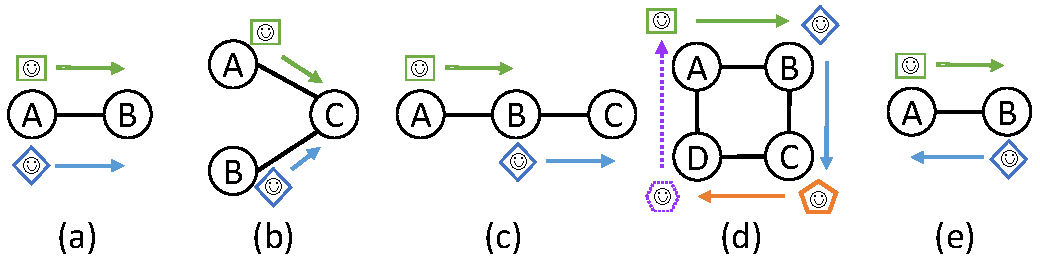
\includegraphics[width=\columnwidth]{types-of-conflicts.pdf}
    \caption{An illustration from~\cite{stern2019mapf} of an edge conflict (a), a vertex conflict (b), a following conflict (c), a cycle conflict (d), and a swapping conflict (e).}
    \label{fig:types-of-conflicts}
\end{figure}

% Conflicts and a valid solution in classical MAPF
A solution to a classical MAPF problem is \emph{valid} if its constituent single-agent plans do not \emph{conflict}. 
An edge conflict between two single-agent plans occurs when the two corresponding agents are planned to perform the same action at the same location at the same time step. 
A vertex conflict occurs when two agents are planned to occupy the same location at the same time. 
A swapping conflict occurs when two agents are planned to swap locations at the same time step. 
Figure~\ref{fig:types-of-conflicts} illustrates these conflicts as well as other types of conflict that arise in classical MAPF. See Stern et al.~\cite{stern2019mapf} for a deeper and more formal discussion of these conflicts. 

%\dor{Why are vertex and swapping conflicts defined between agents and an edge conflict between plans?}\roni{Only edge conflicts are w.r.t plans, and in its text we ``move'' to talking about who is planned to do what. I belive this is clear and easier to read}

% Action cost and objective functions in classical MAPF
In classical MAPF, every action incurs unit cost, 
and the cost of a single-agent plan is the number of its constituent actions. 
\emph{Sum of costs} (SOC) and \emph{makespan} are two common ways to define the cost of a set of single-agent plans $\pi=(\pi_1,\ldots, \pi_k)$. The former is the summation over the costs of the constituent single-agent plans and the latter is their max. A solution to a \mapf problem is called SOC-optimal if it is valid and there is no valid solution that has a smaller SOC. A makespan-optimal solution is defined in a similar way. 
In general, the problem of finding SOC-optimal or makespan-optiaml solutions for a given \mapf problem is known to be NP-Hard~\cite{yu2013multi,surynek2010optimization}.

%, i.e., the plan's length.
%\konstantin{This definition doesn't look nice to me as 'length' may be understood in different ways. May be we come up with another definition?}\roni{Added to elaborate and better explain.}
%Some \mapf algorithms are guaranteed to return a solution with minimal SOC, while others guarantee makespan optimality. \konstantin{I would substitute the last phrase to 'In general solving classical MAPF optimally under either of those objectives is known to be NP-Hard (Yu and LaValle 2016)'.} \roni{Done}

%\roni{Maybe have here also some background on algorithms?}
%\konstantin{May be we add a section here with the overview of the prior work that deals with classical MAPF?}
%\roni{We have that below}

\subsection{Optimal Algorithms for Classical \mapf}
Several approaches have been proposed to find either SOC-optimal or makespan-optimal solutions for classical \mapf 
(e.g., see survey by Felner et al.~\cite{felner2017searchBased}). 
In this work, we build on two specific state-of-the-art classical \mapf solvers: \cbs and MDD-SAT. 
For completeness, we provide a brief description of these algorithms here. 

\subsubsection{Conflict Based Search (CBS)}
\label{sec:cbs}

\cbs~\cite{sharon2015conflict} is a complete and optimal algorithm for classical \mapf. 
It solves a given \mapf problem by finding a plan for each agent separately, detecting conflicts between these plans, and resolving them by replanning for the individual agents subject to specific \emph{constraints}. 

The basic \cbs implementation considers two types of conflicts: a vertex conflict and a swapping conflict. A vertex conflict between plans $\pi_i$ and $\pi_j$ is defined by a tuple $\tuple{i,j,v,t}$, indicating that according to these plans agents $i$ and $j$ plan to occupy $v$ at the same time $t$. A swapping conflict can be defined similarly by a tuple $\tuple{i,j,e,t}$, indicating that according to $\pi_i$ and $\pi_j$ both agents plan to traverse the edge $e\in E$ at the same time, from opposite directions. 
%\dor{Is it an edge conflict or a swapping conflict?}\roni{Good catch}

Correspondingly, the basic \cbs implementation considers two types of constraints. 
A \cbs vertex-constraint is defined by a tuple $\tuple{i,v,t}$ and means that agent $i$ is prohibited from occupying vertex $v$ at $t$.  
A \cbs edge-constraint is defined similarly by a tuple $\tuple{i,e,t}$, where $e\in E$. To guarantee completeness and optimality, \cbs runs two search algorithms: a low-level search algorithm that finds plans for individual agents subject to a given set of constraints, and a high-level search algorithm that chooses which constraints to add. 
%\dor{I think that if we use "vertex-constraint", we should also use "vertex-conflict" (with hyphens).}
%\roni{It depends on context. It is different from how hyphens are used in Hebrew. We can talk about this. Also note it is a swapping conflict but we resolve it by adding an edge constraint.}


%completeness and optimality, \cbs runs two search algorithms: a low-level search algorithm that finds plans for individual agents subject to a given set of constraints, and a high-level search algorithm that chooses which constraints to add. \dor{I think that if we use "vertex-constraint", we should also use "vertex-conflict" (with hyphens).}

%The basic \cbs implementation considers two types of conflicts: a vertex conflict and an edge conflict. A vertex conflict between plans $\pi_i$ and $\pi_j$ is defined by a tuple $\tuple{i,j,v,t}$ and means that according to these plans agents $i$ and $j$ plan to occupy $v$ at the same time $t$. An edge conflict is defined similarly by a tuple $\tuple{i,j,e,t}$, and means that according to $\pi_i$ and $\pi_j$ both agents plan to traverse the edge $e\in E$ at the same time, from opposite directions. \dor{Is it an edge conflict or a swapping conflict?}


% CBS constraints
%A \cbs vertex-constraint is defined by a tuple $\tuple{i,v,t}$ and means that agent $i$ is prohibited from occupying vertex $v$ at $t$.  A \cbs edge-constraint is defined similarly by a tuple $\tuple{i,e,t}$, where $e\in E$. To guarantee completeness and optimality, \cbs runs two search algorithms: a low-level search algorithm that finds plans for individual agents subject to a given set of constraints, and a high-level search algorithm that chooses which constraints to add. \dor{I think that if we use "vertex-constraint", we should also use "vertex-conflict" (with hyphens).}

\paragraph{\textbf{\cbs: Low-Level Search}}
The task of the low-level search in \cbs is to find an optimal plan for an agent 
that is consistent with a given set of \cbs constraints. 
Any single-agent pathfinding algorithm that can do this can be used as the \cbs low-level search. 
To adapt single-agent pathfinding algorithms, such as \astar{}, to consider \cbs constraints, 
the search space must also consider the time dimension since a \cbs constraint $\tuple{i,v,t}$ 
blocks location $v$ only at a specific time $t$. 
This means that a state in this single-agent search space is a pair $(v,t)$, representing that the agent is in location $v$ at time $t$. Expanding such a state generates states 
of the form $(v',t+1)$, where $v'$ is either equal to $v$, representing a wait action, 
or equal to one of the locations adjacent to $v$. States generated by actions that violate the given set of \cbs constraints, are pruned. Running \astar{} on this search space returns the lowest-cost plan to the agent's goal that is consistent with the given set of \cbs constraints, as required. This adaptation of textbook \astar{} is very simple, and indeed most papers on \cbs do not report it and just say that the low-level search of \cbs is \astar{}. 
%\footnote{\textbf{K: Again "A*" is missing. May be we also should say here that enhanced version of A* are also widely used, i.e. the ones that avoid expanding surplus nodes etc. Or I'm not right here?}}. \roni{I'm not sure thus some else did something more fancy than astar}

\paragraph{\textbf{\cbs: High-Level Search}}
The high-level search algorithm in \cbs works on a \ct, which is a binary tree, in which each node
$N$ is defined by a pair $(N.\const, N.\Pi)$ where 
$N.\const$ represents a set of \cbs constraints imposed on the agents and $N.\Pi$ is a \mapf solution consistent with these \cbs constraints. A \ct node $N$ is generated by first setting its constraints ($N.\const$) and then 
computing $N.\Pi$ by running the low-level solver, which finds a plan for each agent subject to the constraints relevant to it in $N.\const$. If $N.\Pi$ does not contain any conflict, then $N.\Pi$ is a valid \mapf solution and $N$ is regarded as a goal node. Else, one of the conflicts $\tuple{i,j,x,t}$ (where $x$ is either a vertex or an edge) in $N.\Pi$ is chosen and two new \ct nodes are generated $N_i$ and $N_j$. Both nodes have the same set of constraints as $N$, plus a new constraint, added to resolve the conflict: $N_i$ adds the constraint $\tuple{i,x,t}$
and $N_j$ adds the constraint $\tuple{j,x,t}$. \cbs searches the \ct in a best-first manner, expanding in every iteration the \ct node $N$ with the lowest-cost joint plan. % with the lowest cost.   

% END COPY AND PASTE FROM WORKSHOP PAPER


\subsubsection{MDD-SAT}
\label{sec:mdd-sat}
A Boolean Satifiability (SAT) problem is defined by a set of Boolean variables $v_1,\ldots v_n$ and a Boolean formula $\Phi$ defined over these variables. 
A solution to a SAT problem is an assignment to these variables such that $\Phi$ is satisfied, or UNSAT if there is no assignment of these variables that satisfies $\Phi$. 

MDD-SAT~\cite{DBLP:conf/ecai/SurynekFSB16} compiles a classical \mapf problem to a sequence of SAT problems. Each SAT problem represents the decision problem: ``is there a valid solution to the given classical \mapf problem with at most $T$ time steps?'' where $T$ is a parameter. $T$ is initially set to one, and incremented one by one until finding the minimal $T$ for which the answer to the corresponding decision problem is ``yes''.  

Every such decision problem is encoded as a SAT problem by defining two types of Boolean variables. The first type, denoted
$\mathcal{X}_{v}^{t}(a_i)$, is defined 
for every discrete time step $t=\{0,\ldots, T\}$, 
agent $i$, 
and vertex $v$ the agent may occupy at time $t$. 
The second type of variable denoted $\mathcal{E}_{u,v}^{t}(a_i)$, is defined 
for every time $t$, agent $i$, 
and edge $(u,v)$ the agent may traverse at time $t$. 
%uses the following decision variables $\mathcal{X}_{v}^{t}(a_i)$ and $\mathcal{E}_{u,v}^{t}(a_i)$ for discrete time-steps $t \in \{0,1,2, ...\}$ describing occurrence of agent $a_i$ in $v$ or the traversal of edge $\{u,v\}$ by $a_i$ at time-step $t$. 
\mapf movement rules and collision avoidance constraints are encoded on top of these variables as simple local constraints. 
The resulting Boolean formulae is given to a SAT solver, which returns either a satisfying assignment or UNSAT. A satisfying assignment to the decision variables specifies a valid solution for the given \mapf problem. An UNSAT indicates no valid solution exists within $T$ timesteps, in which case $T$ is increased by one. 
This approach returns makespan optimal solutions, and with some additional bookmarking can also be used to return sum-of-costs minimal solutions. 


\roni{Since we say we use MDD-SAT, maybe we need to elaborate a bit more here about the MDD part. At least, to say that MDD-SAT is based on the above encoding, but also use a multi-valued decision diagram to remove decision variables that can be predicted apriori to be false. Pavel/Konstantin, what do you think?} 
\konstantin{I agree. Right now it is not evident what MDD means in the algorithm name. The text we have just describes 'sequential SAT' approach for classical MAPF}




\subsection{Limitations of Classical MAPF and Prior Work on General MAPF}
\label{sec:limitations}
%5TODO: Konstantin
%Typically the \ac{MAPF} problem is formulated as a graph search problem, i.e. all agents are confined to the graph $G=(V, E)$, which vertices correspond to the locations in the environment and the edges -- to the feasible transitions between the locations. The time is discretized into the timesteps and it is assumed that at each time step an agent can either wait at the vertex or move from this vertex to some of its neighbors, following a certain edge. The path for an agent is formally a mapping from the timesteps to the graph vertices: $\pi = T \rightarrow V$, where $T=[0, 1, 2, ...]$, s.t. each two consecutive timesteps are mapped either to the same vertex (the agent is waiting) or to the two adjacent vertices (the agent is moving). Because the time is discretized an agent can be though of as teleporting from one vertex to the other (or to the same vertex, in case of the wait action).
%In case only one agent is present in the environment (on the graph), each its path is feasible, i.e. no collision occurs while agent is following it. This is due to the assumption that each edge resembles a collision-free transition between the neighboring vertices. In the multi-agent setting, obviously, collisions might occur between two (or more) agents' paths and one need to define them appropriately. In \cite{} the most common definitions of the conflicts for time-discretized graph-based MAPF are given: vertex conflict, edge conflict, following conflict, cycle conflict and swapping conflict. It is important to note that all of them are tied to the exact discrete timestep and to the graph edge or vertex. E.g. a swapping conflict occurs if there exist a timestep $t$: $\pi_1(t)=\pi_2(t+1)$ and $\pi_2(t)=\pi_1(t+1)$.

%\textbf{K: Maybe a picture from SoCS'19 paper showing all classical conflicts here?}\roni{Done}
%Having the notion of the individual path and the conflict the (time-discretized) MAPF problem can be stated as the problem of finding a set of individual paths (from predefined start locations to the predefined goal locations) such that each pair of them is conflict-free. The objective is, commonly, to minimize either the \textit{makespan}, i.e. the time when the last agent reaches its goal\footnote{by saying ``reach the goal'' we mean that the agent comes to the goal vertex and does not move out of it in any further timestep.}, or the \textit{sum-of-costs}, i.e. the sum of timesteps each agent has spent on reaching its goal across all the agents. It is known that solving MAPF optimally under both objectives is NP-hard \cite{}.


%While much work has been done on classical \mapf, an important question is how well it relates to real-world \mapf applications, e.g. in a robotics setup when a group of mobile robots have to safely navigate in the shared environment. In particular, consider the following intrinsic simplifying assumptions of classical \mapf and their implications. 
%Moving mobile robots is commonly assumed motivation for work on \mapf

Moving a group of mobile robots safely in a shared environment is commonly considered as a primary application for a \mapf research. An important question is therefore how the definition of a classical \mapf problem relates to real-world \mapf applications in robotics. In particular, consider the following intrinsic simplifying assumptions of classical \mapf and their implications in robotics. 
%Moving mobile robots is commonly assumed motivation for work on \mapf


\begin{itemize}
    \item \textbf{A1. The duration of every move action is one time step.} 
    This means either all agents move in exactly the same speed and graph edges represent transitions of the same length,
    or that graph edges represent transitions of different lengths and the agents adapt their velocity and acceleration profile so that all moves take one time step. 
    %\dor{We need to use either "time-step", "time step", "time", or "timestep".}\roni{Time step. Note that in some cases we do need to add the hyphen}
    %    Also, wait actions are     4-connected grids are the most suitable models aligned with the discussed assumption. No wonder, the majority of the priory introduced MAPF planners were evaluated on them. The planners that go beyond this setting and can work on the graphs with the edges of non-uniform duration are also    so that the agents  following them accomplish the move in the same time (equal to 1 timestep); or the graph edges can be of different lengths but the agents have an embedded mechanism of choosing the correct velocity/acceleration profile to perform a move within 1 timestep. 4-connected grids are the most suitable models aligned with the discussed assumption. No wonder, the majority of the priory introduced MAPF planners were evaluated on them. The planners that go beyond this setting and can work on the graphs with the edges of non-uniform duration are also known ???????????????????
    \item \textbf{A2. The duration of a wait action is one time step.} 
    This means an agent may wait any discrete number of time steps, as oppose to any real valued duration. 
    %Allowing wait actions with arbitrary duration is challenging as it means there exist an infinite number of wait actions in each location. \roni{Out of context now.}
    %This poses a problem if one wants to apply a conventional heuristic search algorithm that relies on generating (or at least enumerating) all the successors of any search state. Luckily, there exist a technique that can be adopted to reason about the actions of arbitrary duration -- Safe Interval Path Planning (SIPP) \cite{}. It has already been used in the MAPF domain \cite{}, but only within a prioritized approach, that is known to be incomplete in general. 

%    \item \textbf{A3. All agents use the same graph ($G$).}      All agents move along the same edges and can stop in the same predefined locations (vertices).      This implies that in the real-world they should have (roughly) the same size and shape, and adhere to the same kinodynamic constraints.      Otherwise, some move actions may be feasible for some agents (e.g., small agents) and lead to collisions with static obstacles for other agents (e.g., large agents).    
\end{itemize}
%\roni{I swapped the order, since we mostly talk about the first two}
%\roni{I wonder if we want to say something here about agent sizes and shapes}
%Agents also should adhere to the same kinodynamic constraints to perform vertex to vertex transitions in the same manner, so the assumption that there exist a single edge between the pair of adjacent graph vertices holds true.
%In this work we lift all three assumptions. For ease of exposition we first restrict our discussion to lifting the first two assumptions, and assume all agents are of the same shape and size. We discuss later how to lift these two assumption (A3 and same-shape).
%For ease of exposition we first restrict our discussion to lifting the first two assumptions, and assume all agents are of the same shape and size. We discuss later how to lift these two assumption (A3 and same-shape). 
%Others have also considered lifting these specific simplifying assumptions. Next, we describe these prior works and the relation between then, before defining the exact \mapf problem we address. 
%Others have also considered lifting these specific simplifying assumptions. Next, we discuss these prior works, and then define exactly the type of \mapf problem we address, which we refer to as \mapf in Euclidean space with continuous time (\mapfect). 
%, before defining the exact \mapf problem we address. 
%Before defining it, we discuss  and define it below. 
%To do so we, first, state the continuous time MAPF problem when all agents are confined to the same graph; present an optimal algorithm of solving it; show how the latter can be applied to the heterogeneous MAPF statement, when the agents are operating on the different graphs. \roni{I think all the above (now connected) should go to the intro, and perhaps in a briefer way.}


%subsection{Prior Work on General MAPF}

%\roni{Below I describe almost word-to-word the models used by Thayne and Liron. Let's discuss this next time we talk}

In this work we lift these assumptions. 
Since we are not the first to do this, we first discuss prior works and the relation between them. 
% MAPFR
%Others have also considered lifting these specific simplifying assumptions. 
Walker et al.~\cite{walker2018extended} introduced the \mapfr problem, which lifts the first classical \mapf assumption (AS1). 
In \mapfr, every edge $e=(v,v')$ in the underlying graph $\mathcal{G}$ is associated with a positive weight $w(e)\in \mathbb{R}_{>0}$ that represents the duration it takes an agent to move from $v$ to $v'$. 
Every location $v\in V$ is associated with a unique coordinate in a metric space, denoted $\coord(v)$. 
An agent is a circle with a non-zero volume. 
When the location of an agent is $v$, it means the center of the agent is located at $\coord(v)$. 
When an agent moves along an edge $(v,v')$, it means
its center moves along a straight line from $\coord(v)$ to $\coord(v')$ in a constant velocity motion. 
There is a conflict between two single-agent plans iff the volumes of ``one or more agents overlap at the same instant in time''~\cite{walker2018extended}. This can be detected using standard collision detection techniques~\cite{helpHere}. 

% Limitation of MAPFR
To solve \mapfr, however, Walker et al.~\cite{walker2018extended} proposed the Extended Increasing Cost Tree Search (E-ICTS) algorithm, which can guaranteed  optimal or  bounded-suboptimal solutions. 
The definition of \mapfr does not specify the duration of wait actions. 
Thus, it is not clear whether \mapfr also lifts the second assumption (A2) by allowing arbitrary wait actions. The E-ICTS algorithm, however, requires accepting the duration of wait actions as a parameter. 



% Multi-agent motion planning
Cohen et al.~\cite{cohen2019optimal} proposed a relevant extension of classical \mapf that they called \emph{multi-agent motion planning} (MAMP).  In MAMP, each agent is associated with a graph $\mathcal{G}_r=(V_r,E_r)$. 
A vertex in $V_i$ represents a possible \emph{state} of agent $r$, where a state of an agent represents its location as well as other relevant features such as orientation and steering angle. 
An edge $e_r=(v,v')\in E_r$ represents a kinodymaically feasible motion of agent $r$ from state $v$ to state $v'$, 
and the weight of an edge is the duration of performing this motion.
%Importantly, the sets of cells associates with states of different agents may intersect, thereby indicating a potential conflict. 
The agents in MAMP move in an \emph{environment} represented by a list of cells $\mathcal{C}$. 
Every state $v\in V_r$ of an agent $i$ is associated with a set of cells in $\mathcal{C}$, representing the cells occupied by that agent when in state $v$. 
Every edge $e_r=(v,v')\in E_i$ is associated with a multiset of cells in $\mathcal{C}$. 
Each cell in this multiset is associated with a time interval indicating the time interval in which this cell is occupied when agent $r$ moves from $v$ to $v'$.

% Limitation of MAMP
Cohen et al.~\cite{cohen2019optimal} proposed an optimal and a bounded-suboptimal algorithm for solving MAMP problems, based on Conflict-Based Search (CBS)~\cite{sharon2015conflict}. Their algorithm, called CBS-CT, is designed to lift the second classical \mapf assumption (AS2), allowing arbitrary duration for wait actions. 
However, it relies on the discretized representation of the environment into a set of cells ($\mathcal{C}$). Thus, while it allows move actions with non-unit duration (addressing AS1), its efficiency and relation to the real-world depend on this discretization of the environment. Every such discretization introduces inaccuracy and potential for incompleteness: an optimal solution for one discretization may not be optimal for another, and a problem may be solvable under one discretization and unsolvable under other discretization.  
The algorithms we propose are fundamentally different in that they do not require a discretization of the environment into grid cells.  Thus, they require a different problem definition than MAMP. 


\section{Problem Statement}

The \mapf problem we address in this work can be viewed as \mapfr, but where wait actions can have an arbitrary duration.  
We define a \mapfr problem by the tuple $\langle \mathcal{G}, \mathcal{M}, \source, \target, \coord, \mathcal{A}\rangle$ 
where $\mathcal{G}=(V,E)$ is a graph, 
$\mathcal{M}$ is a metric space, 
%\konstantin{maybe we change M to $\mathcal{M}$?}, roni:odne
$\source$ and $\target$ are the start and goal functions, 
$\coord$ maps every vertex in $\mathcal{G}$ to a coordinate in $\mathcal{M}$, 
and $\mathcal{A}$ is a finite set of possible \emph{move actions}.



%A \emph{collision} occurs when agents' shapes overlap.  To detect such an overlap, we assume a \emph{collision-detection} method $\iscollision:\{1,\ldots,k\}\times \{1,\ldots,k\}
%\times \mathcal{M}\times \mathcal{M}
%\rightarrow \{\true,\false\}$ 
%is available where \iscollision($i,j,m_i,m_j$)=$\true$ iff when agents $i$ and $j$ occupy locations $m_i$ and $m_j$, respectively, then their shapes overlap. 
%For example, if the agents are disk-shaped with a radius of $r$, then conflict occurs between two single-agent plans if there exists a point in time for which the distance between the coordinates associated with the agents following these plans are less than $2r$ distance apart. 
%That is, in this setting, 
%\begin{equation}
%\iscollision(i,j, m_i,m_j)=
%\begin{cases}
%\true & ||m_i-m_j||_2\leq 2r \\
%\false & \text{Otherwise}
%\end{cases}
%\end{equation}
%Note that our problem definition and the algorithms we propose later are not restricted to disk-shaped agents and this particular type of \iscollision implementation. 





Every action $a$ in \mapfr is defined by a duration $a_D$ and a \emph{motion function} $a_\varphi$. 
A motion function $a_\varphi$ is a function $a_\varphi:[0,a_D]\rightarrow \mathcal{M}$, that maps time to metric space. Here $a_\varphi(t)$ is the coordinate of an agent (in $\mathcal{M}$) at the time $t$ while executing an action $a$.
%in $M$ an agent reaches $t$ time after starting to perform $a$. 
There are two types of actions in \mapfr: move actions and wait actions. 
For a move action $a\in \mathcal{A}$, we restrict $a_\varphi$ so that it starts in some vertex $v$, 
ends in some other vertex $v'$, and $(v,v')$ is an edge in $E$. 
That is, there exists $v$ and $v'$ such that $a_\varphi(0)=\coord(v)$, $a_\varphi(a_D)=\coord(v')$, and $(v,v')\in E$.
%\dor{Maybe we should define the location of the agent on the edge between these two times.}\roni{We already say this above when we define the motion function}
A \emph{wait action} $a$ is an action for which there exists a vertex $v\in V$ such that for every $t\in [0,a_D]$ 
we have that $a_\varphi(t)=\coord(v)$. Note that while the set of move actions is given as input ($\mathcal{A}$), 
the set of wait actions is implicitly defined for every vertex $v\in V$ and \emph{any} positive real number $a_D$. 
Thus, the set of wait actions is infinitely large.
In \mapfr, when an agent is at a vertex $v$ it can choose to perform any action -- move or wait -- that starts at $v$, i.e., $a_\varphi(0)=\coord(v)$. 

A \emph{collision} between the agents occur if their shapes overlap. To detect such an overlap, we assume a \emph{collision-detection} method $\iscollision:\{1,\ldots,k\}\times \{1,\ldots,k\}
\times \mathcal{M}\times \mathcal{M}
\rightarrow \{\true,\false\}$ 
is available where \iscollision($i,j,m_i,m_j$)=$\true$ iff when agents $i$ and $j$ occupy locations $m_i$ and $m_j$, respectively, then their shapes overlap. For example, if the agents are disk-shaped with a radius of $r$, then a collision occurs if the distance between the centers of the agents is less than $2r$. That is, in this setting, 
\begin{equation}
\iscollision(i,j, m_i,m_j)=
\begin{cases}
\true & ||m_i-m_j||_2 < 2r \\
\false & \text{Otherwise}
\end{cases}
\end{equation}
Note that our problem definition and the algorithms we propose later are not restricted to disk-shaped agents and this particular type of \iscollision implementation. 


% Sequences of actions
For a sequence of actions $\pi=(a_1,\ldots, a_n)$, 
we denote by $\pi[:j]$ the prefix of the first $j$ actions, i.e., 
$\pi[:j]=(a_1,\ldots a_j)$. The duration and motion function of $\pi$, denoted 
$\pi_D$ and $\pi_\varphi$, respectively, are defined as follows: 
\begin{equation}
    \pi_D=\sum_{a\in\pi} a_D
\end{equation}
\begin{equation}
    \pi_\varphi(t)=
    \begin{cases}
        {a_1}_\varphi(t)  & t\leq {a_1}_D \\
        \cdots & \cdots  \\
        {a_j}_\varphi(t-(\pi[:j-1])_D) & (\pi[:j-1])_D < t \leq (\pi[:j])_D \\
        \cdots & \cdots  \\
%        {a_n}_\varphi(t-\pi[:n-1]_D) & \pi[:n-1]_D < t \leq \pi_D \\
        {a_n}_\varphi(t-(\pi[:n-1])_D) & (\pi[:n-1])_D < t \leq (\pi[:n])_D \\
        {a_n}_\varphi({a_n}_D) & (\pi[:n])_D < t \\
        
    \end{cases}
    \label{eq:motion}
\end{equation}

%\roni{There is some ugliness in that the last range is unbounded. This is intentional as I need it later}
%\konstantin{Does this equation (correctly) describe the location of an agent after the plan is executed?}.
%\roni{ Location after plan is done - depends on our assumption: if the agent stays there then yes (I think we want this for later, let's discuss)}
%\konstantin{I still think that the last line of the eq. is formally incorrect. E.g. the duration of the plan is 20 and the plan itself is a sequence of two actions whose durations are 10. Assume now that $t=25$. 25 is greater than 20, so the last line holds. So now I apply the motion function that describes the last action with the argument 25-10, which is 15. But the last action is not defined for the $t=15$ as its duration is 10.}
%\roni{Got it, added another line to define that after the plan ends, the agent is assumed to stay in its last location.}

Te explain Equation~\ref{eq:motion}, which computes the location at each time moment while executing $\pi$, observe that the motion functions are not defined with respect to when their respective actions are applied. For instance, for any action $a$ that moves the agent from $v$ to $v'$, by definition $a_\varphi(0)=v$ and $a_\varphi(a_D)=v'$.
%\konstantin{should not it be $a_\varphi(a_D)=v'$?}\roni{Fixed}
Therefore, to compute $\pi_\varphi(t)$ we need to first identify the action planned to be executed at time $t$. 
This can be computed by observing that the $i^{th}$ action in $\pi$ starts at time $(\pi[:i-1])_D$ and ends at time $(\pi[:i])_D$ for every $i>1$. 
Then, we ``correct'' $t$ by the starting time of that action, to obtain the location of the agent during the execution of that action. 
The last line in Equation~\ref{eq:motion} defines that the agent is assumed to stay in its last location after the plan ends. 


% Collision detection
%\konstantin{May be we shift 'collision detection' part up, e.g. after the 2nd paragraph of Problem Statement. The reason is that Collision detection somehow 'cuts' the narration concerning plans and conflicts between the plans.}\roni{Fixed}


% Connecting single agent plans and collisions gets a  conflict.

As in classical \mapf, we define a single-agent plan for an agent $i$ to be a sequence of actions $\pi=(a_1,\ldots, a_n)$ 
such that executing it moves agent $i$ from $\source(i)$ to $\target(i)$. 
A \emph{conflict} between two single-agent plans is naturally defined as the case where if they agents execute their respective plans starting at the same time then there exists a point in time in which a collision occurs. 

\begin{definition}[Conflict in \mapfr]
Two single-agent plans $\pi_i$ and $\pi_j$ have a conflict iff 
\begin{equation}
    \exists t\in [0, \max({\pi_i}_D,{\pi_j}_D)] 
        ~~ \iscollision\big(i,j,{\pi_i}_\varphi(t), {\pi_j}_\varphi(t)\big)
\end{equation}
\label{def:conflict-mapfr}
\end{definition}


%the shapes of agents $i$ and $j$ overlap if $i$ is at $m_i$ and $j$ is at $m_j$ at the same time. 
%\konstantin{Why there is a 'conflict' in the name of 'collision' detection function. I suggest renaming to InCollision}\roni{I changed the isconflict macro so that it outputs iscollision as you suggested.}
%\konstantin{Why do mention time? InCollision does not dependent on time according to the definition}
%\roni{Fixed}

%\konstantin{Intuitively, this is understandable. Formally it's not defined so far what is 'point in time' when we are speaking about the plans}
%\konstantin{May be we need here something here that will tie together 'collision detection' which is not dependent on time and 'agent exetuing a plan' which is strongly dependent on time. I mean: Ok, we have two plans and a collision-detection function. How to apply this function in order to claim that these two plans do conflict with each other.}
%\roni{I liked this idea and did it. Let me know if it works}


A solution to a \mapfr is valid if all its constituent single-agent plans do not conflict. The cost of a single-agent plan is its duration. Like in classical \mapf, the sum of costs of a solution is the sum of costs (SOC) of its constituent single-agent plans, and the makespan of a solution is the maximum over these costs. 
Correspondingly, we define two problems: 
the problem of finding a SOC-optimal solution to a \mapfr problem and the problem of finding a makespan optimal solution to a \mapfr problem. In this work, we 
consider both problems and propose algorithms for solving them. 


%the two corresponding problems: the problem of finding a SOC-optimal solution to a given \mapfr problem and the problem of finding a makespan-optimal solution. We propose algorithms for both problems.

%Overall, the problem we are interested in this work can now be formulated as follows. Given a \mapfr problem $\langle \mathcal{G}, \mathcal{M}, \source, \target, \coord, \mathcal{A}\rangle$ find a valid solution that having an optimal cost. 
%Different objective functions for \mapfr may also be proposed, e.g., makespan, which is the maximum over the duration of all the plans comprising solution.

%Overall, the problem we are interested in this work can now be formulated as follows. Given a \mapfr problem istance $\langle \mathcal{G}, \mathcal{M}, \source, \target, \coord, \mathcal{A}\rangle$ find a valid solution that is sum-of-costs and/or makespan optimal.

%\konstantin{I added the above paragraph because before it was not said explicitly what kind of solutions are we striving for.}

\begin{figure}
    \centering
    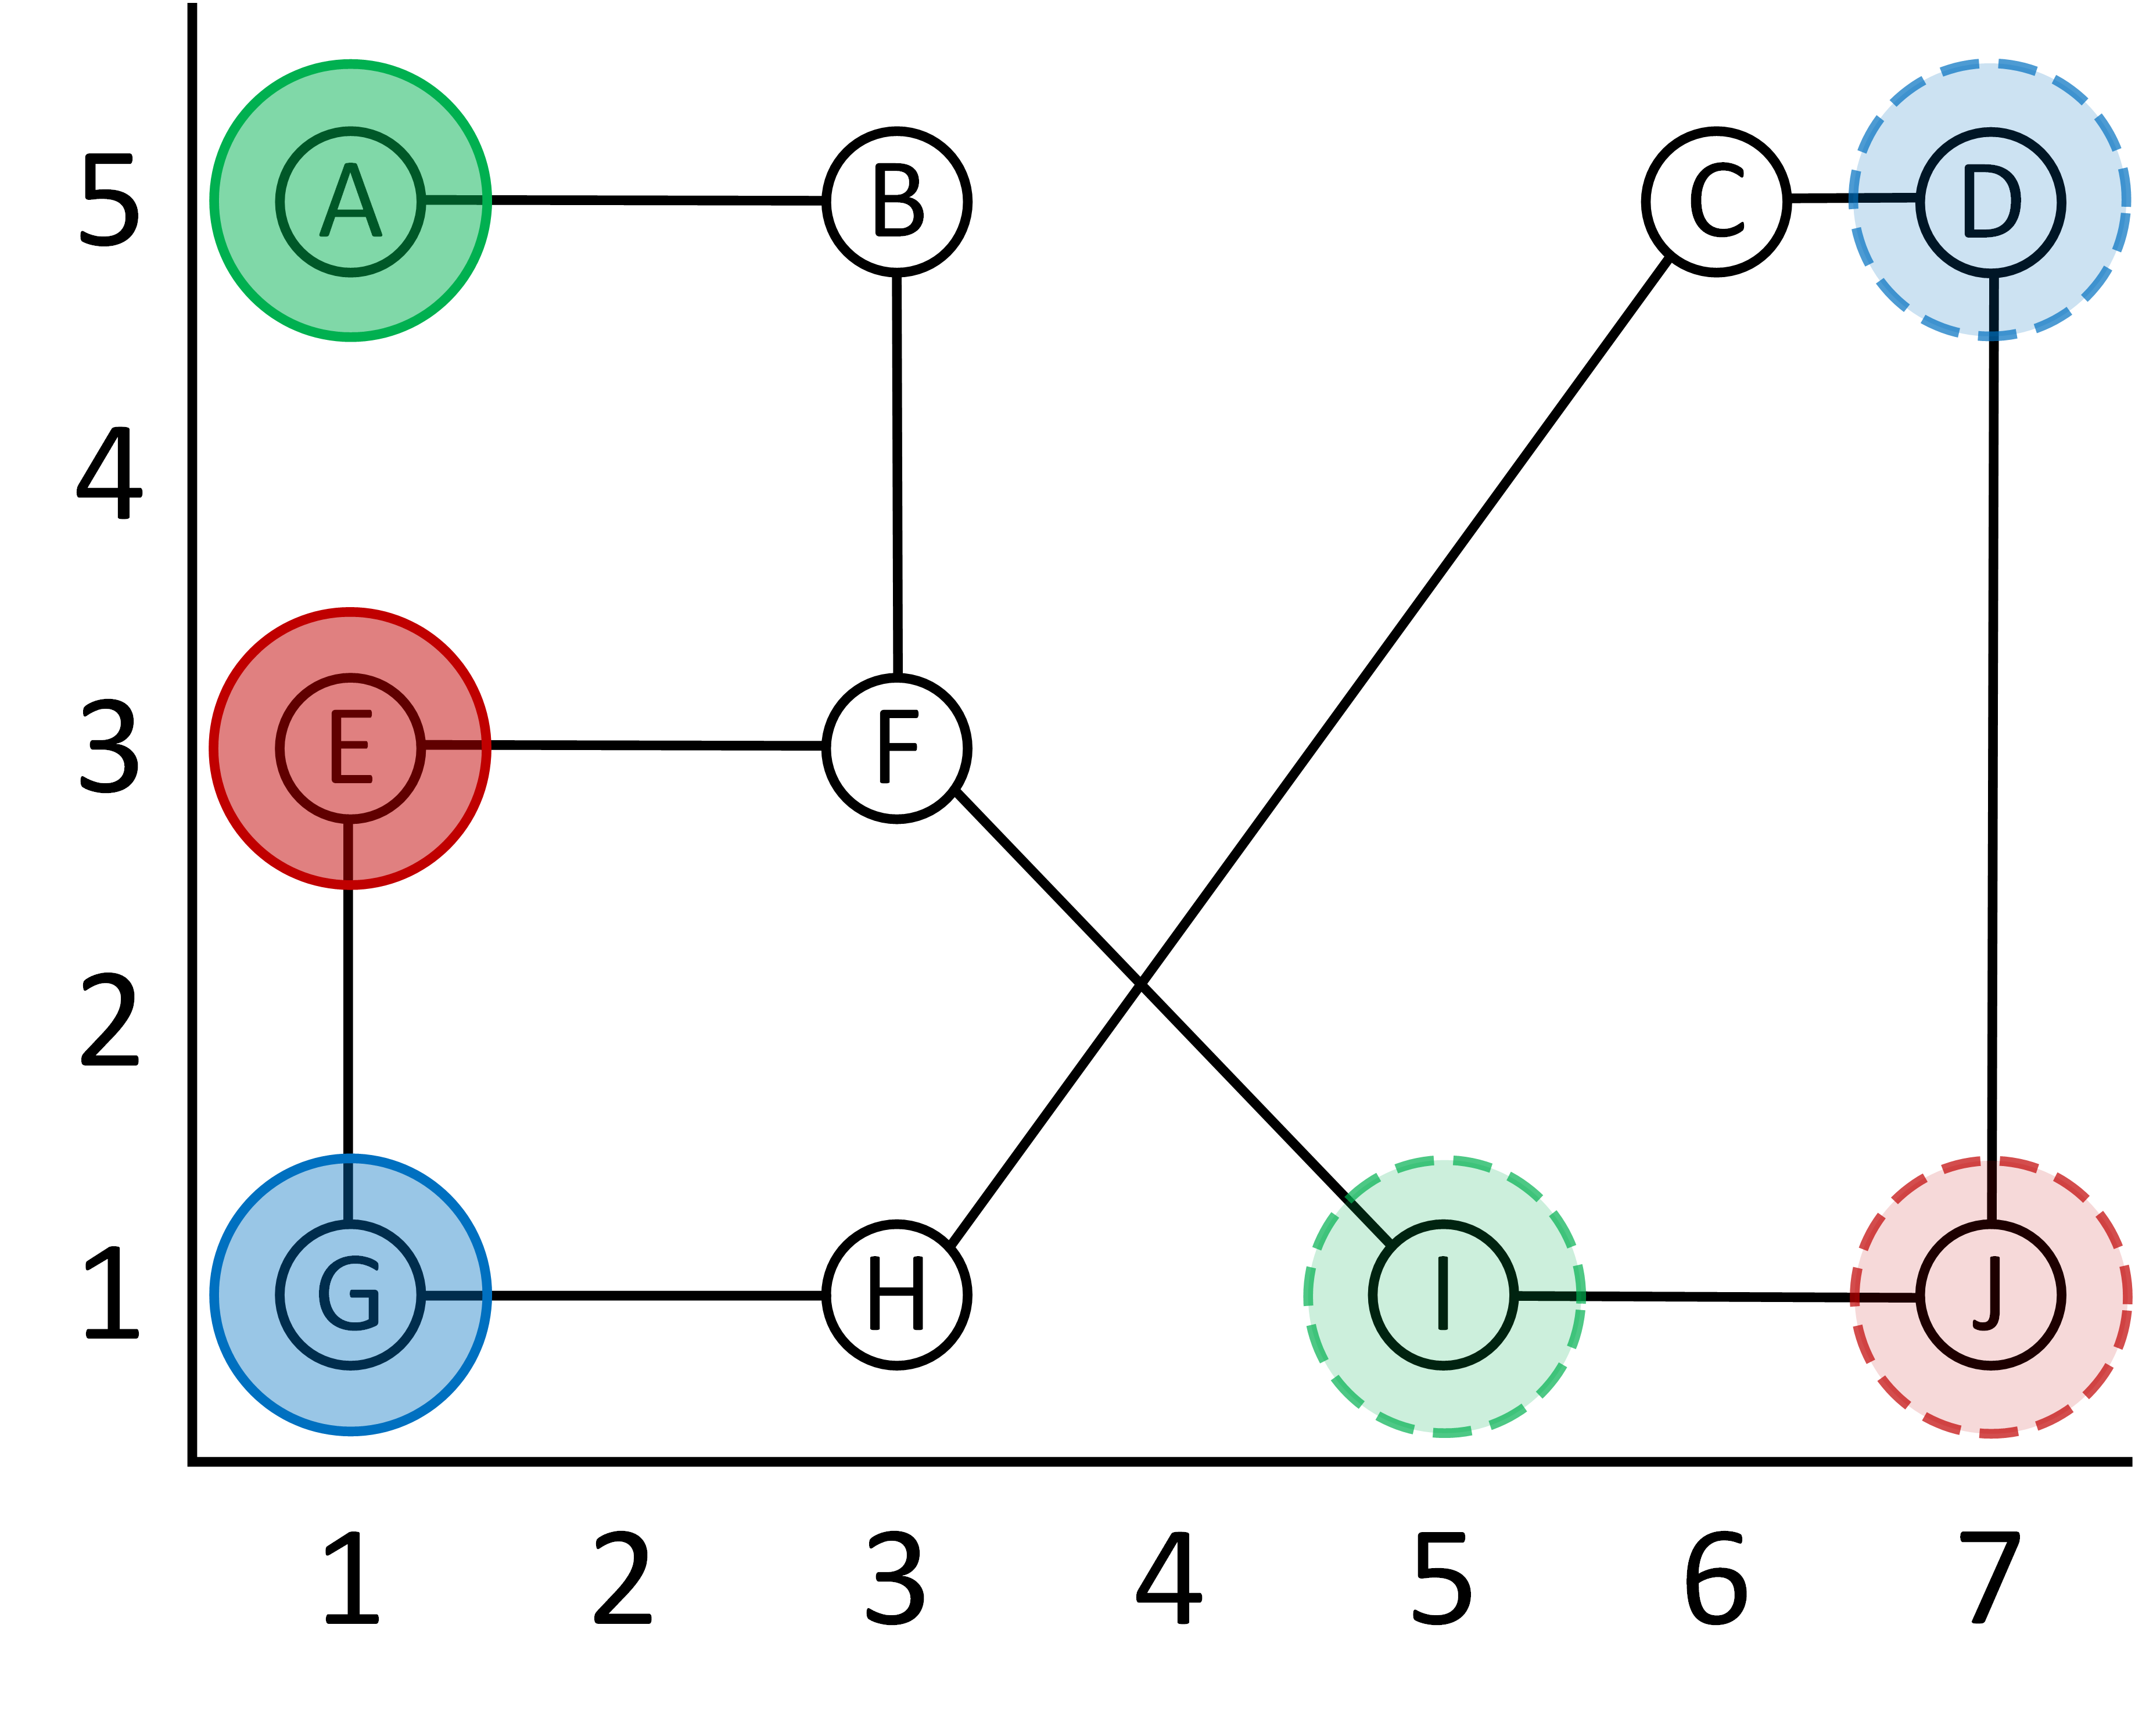
\includegraphics[width=0.6\columnwidth]{running_example.png}
    \caption{Our running example: \mapfr problem with 3 agents.}
    \label{fig:example}
\end{figure}

\begin{figure}
    \centering
    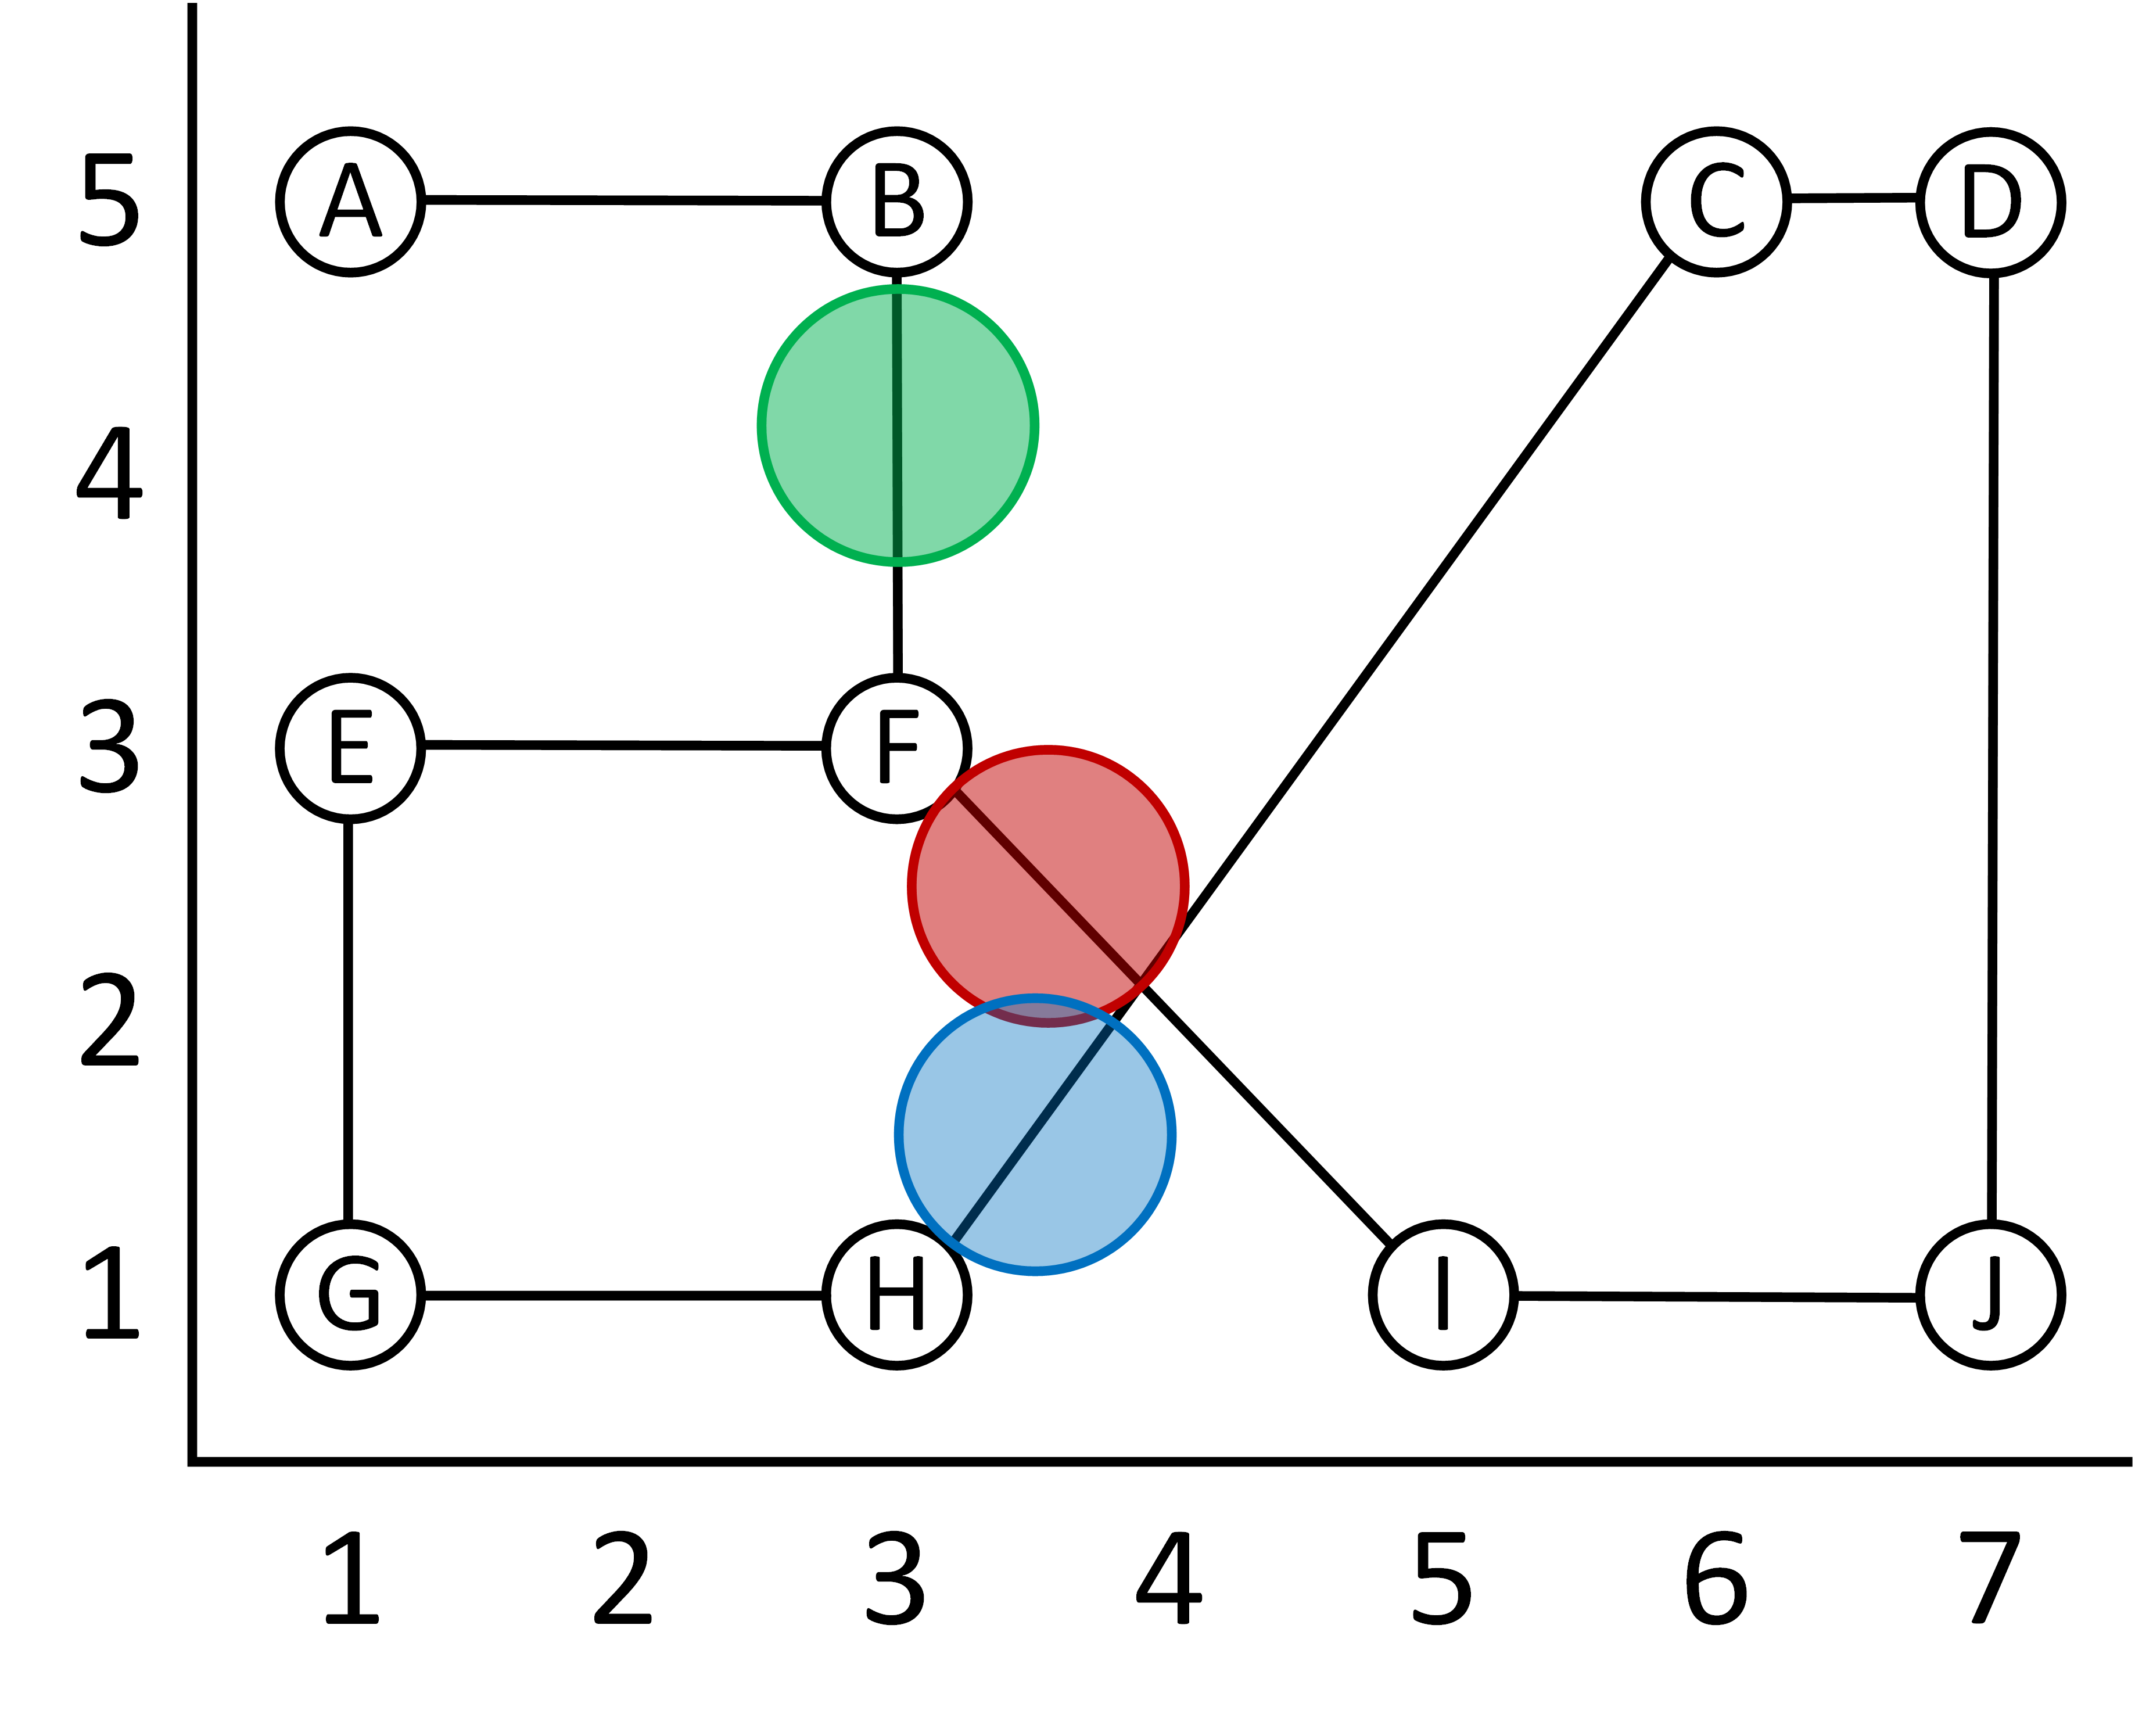
\includegraphics[width=0.6\columnwidth]{running_example_t2-8.png}
    \caption{Positions of the agents following their individual plans at time moment $t=2.8$. Red and blue agents are in collision.}
    \label{fig:example-t-2-8}
\end{figure}

\subsection{\mapfr Example}
Figure \ref{fig:example} shows an example \mapfr problem. 
Small circles with the letters inside them denote graph vertices, e.g. vertex $A$ corresponds to a point with the coordinates $(1, 5)$, straight line segments between vertices depict edges. %, e.g. vertex $C$ is reachable from $H$ by following the segment that starts at $(3, 1)$ and ends at $(6,5)$. 
Agents are shown as colored circles. Each agent is a disk with a radius of 0.5. Initially the green agent occupies vertex $A$, the red agent -- vertex $E$, and the blue agent -- vertex $G$. Their respective goals are $I$ (green agent), $J$ (red agent), and $D$ (blue agent).

10 move actions, corresponding to 10 graph edges are present in this setting (with the infinite number of the wait actions). Assume the agents' moving speed is one; they start and stop instantaneously; and move from one vertex to the other following the straight line segment connecting them. Thus, the duration of every action equals the distance between the vertices that define that move action. E.g. duration of the action ``move from $A$ to $B$'', denoted as $A \rightarrow B$, is 2. The motion function that describes this action is: $(A \rightarrow B)_\varphi(t) = \overrightarrow{OA} + {1\over{||AB||}} \cdot \overrightarrow{AB} \cdot t$.

The least-cost individual plans to the agents' respective goals are: $\pi_{green}=\{A \rightarrow B, B \rightarrow F, F \rightarrow I\}$ for the green agent; $\pi_{red}=\{E \rightarrow F, F \rightarrow I, I \rightarrow J\}$ for the red agent; $\pi_{blue}=\{G \rightarrow H, H \rightarrow C, C \rightarrow D\}$ for the blue one. If the agents start executing them simultaneously, then at $t=2.8$ their positions will be $(3, 4.2)$, $(3+0.4\cdot \sqrt{2}, 3-0.4\cdot \sqrt{2})$, $(3.48, 1.64)$  respectively (see Figure \ref{fig:example-t-2-8}). The distance between the positions of red and blue agent is less that the sum of their radii, thus, they are colliding and their plans are in conflict. 

%Our aim is to avoid collisions between the agents by finding plans that are conflict-free. In this work we strive for sum-of-costs (or makespan) optimal solutions.
%[[Roni: removed this following our discussion]] \konstantin{Need to check the last sentence in the paragraph above after we finalize problem statement.}\roni{The above part repeats what was said. This is an exmaple, not a problem definition. We have the problem definition above. 


%The least-cost individual plans to the agents' respective goals are: $\pi_{green}=\{(A \rightarrow B, 0), (B \rightarrow F, 2), (F \rightarrow I, 4)\}$ for the green agent; $\pi_{red}=\{(E \rightarrow F, 0), (F \rightarrow I, 2), (I \rightarrow J, 2+2\sqrt{2})\}$ for the red agent; $\pi_{blue}=\{(G \rightarrow H, 0), (H \rightarrow C, 2), (C \rightarrow D, 7\}$ for the blue one. If the agents start executing them simultaneously, then at $t=XXX$ their positions will be $(X, Y)$, $(X, Y)$, $(X, Y)$  respectively (see \ref{fig:example-t-X}). The distance between the positions of $X$ and $Y$ is less that the sum of their radii, thus, they are colliding, thus their plans are in conflict. Our aim is to avoid collisions of the agents by finding plans that are conflict-free. In this work we strive for sum-of-costs (or makespan) optimal solutions.



%\roni{The above: we need to change $G$ in the figure to avoid confusion with the goal function.}
%\konstantin{I think this will ruin some figures Pavel already made. We also have a figure (see. '$running\_example\_tree$' that is dependent on the graph vertex 'G'. May be we keep it as is for now (at least for the initial submission)? }
%\roni{Yes, not important.}


\section{Conflict-Based Search with Continuous Time}

% COPY AND PASTE FROM WORKSHOP PAPER
In this section, we introduce \ccbs -- an algorithm that finds SOC-optimal solutions to  \mapfr. 
It is based on two algorithms: \cbs~\cite{sharon2015conflict} and \sipp~\cite{phillips2011sipp}. 
For completeness, we provide a brief relevant background on \sipp before introducing \ccbs. 
%\konstantin{Didn't we want to give a background on CBS as well? I think we had such text at some stage. Why did we marked it out?}\roni{It was moved to the background section.}


\subsection{\sipp}
\sipp~\cite{phillips2011sipp} is a powerful algorithm for building a plan for a single agent moving among static and dynamic obstacles~\cite{phillips2011sipp}. 
It has also been used within prioritized \mapf solvers \cite{yakovlev2017anyAngle} and for solving multi-agent pickup and delivery problems \cite{ma2019lifelong}. 
%and later enhanced in the works \cite{}, \cite{}. 
%In this work we use SIPP as a single-agent planner inside the CBS framework, however it can also be used within prioritized MAPF solvers \cite{yakovlev2017anyAngle}, for solving Multi-agent Pickup and Delivery problems \cite{ma2019lifelong}, etc.
\sipp accepts as input a graph, a start and goal vertices in that graph, and trajectories specifying the motion of the dynamic obstacles over time. 
The algorithm pre-processes these trajectories to compute \emph{safe intervals} for each vertex in the graph. 
A safe interval is a contiguous period of time for a vertex, during which if the agent occupies that vertex then it will not collide with any dynamic obstacle. 
Safe intervals are assumed to be maximal, i.e. extending a safe interval is not possible.

For example, consider a case where only one dynamic obstacle is present and both an agent and the obstacle are disks of radius $r$.
Now, consider a vertex $v$ such that the distance between this obstacle and $v$ is less than $2r$ between time moments $t_1$ and $t_2$. The corresponding safe intervals for $v$ are $[0, t_1]$ and $[t_2, +\infty)$.
Note that in this example, we assume that (1) a collision happens only when the distance between two disks is less than the sum of their radii, when the distance is equal to it -- no collision happens; and (2) the collision does not occur at the specific point $t_1$ and $t_2$.

A vertex may have multiple, non-overlapping, safe intervals. 
In general the number of safe intervals is proportional to the number of the obstacles that pass nearby the vertex. The chronologically last safe interval for a vertex might end not with the $\infty$ -- e.g. some obstacle comes to this vertex and stays in it. The safe interval might be an $\emptyset$ as well -- consider e.g. an obstacle that constantly moves back-and-forth in the vicinity of the vertex. 



\sipp performs an \astar-like search over the search space in which each node is a pair of graph vertex and one of its safe intervals. This means there may be multiple search nodes for the same vertex but with different safe time intervals. In the example above, nodes
%$n_1=\langle v, [0, t_1] \rangle$ and $n_2=\langle v, [t_2, +\infty) \rangle$ 
$n_1=(v, [0, t_1])$ and $n_2=(v, [t_2, +\infty) )$ 
correspond to the same vertex $v$, but have different safe intervals.
Guided by a consistent heuristic, \sipp is guaranteed to return optimal solutions. 
Sub-optimal and anytime variations of the algorithm are also known \cite{narayanan2012anytime,yakovlev2020revisiting}. %, but in this work we use the basic, optimal, \sipp. 

%Next we describe the main ideas of SIPP. Without the loss of generality we will consider both the agent and the obstacles to be disks of the same size (radius equals $r$).
%The crux of the method is the notion of the safe interval for a graph vertex~\cite{phillips2011sipp}. The latter \dor{Out of whom?} is a contiguous period of time for a vertex, during which no collision happens with the dynamic obstacles if an agent occupies the vertex. Safe intervals are opposed to collision intervals, and are assumed to be maximal, i.e. extending a safe interval is not possible.


%For each node in its search space, \sipp maintains a $g$-value -- the cost of the best-known plan that ends at this vertex, an $h$-value -- a heuristic estimate of the cost to the goal, $parent$ -- the predecessor node in the search-tree, and the earliest possible time within the safe interval the node can be reach from $parent$. In the considered domain, $g(n)$ and $EAT(n)$ are equivalent as the cost of a plan is the time the agent needs to execute it. Earliest possible arrival time for a node is computed when its predecessor is expanded. Being a planning algorithm, \sipp assumes that the exact procedure of computing this time moment is available.\roni{What is this time moment? not clear} 



\subsection{From \cbs to \ccbs}

\ccbs follows the \cbs framework. %: it has a low-level search algorithm that finds plans for individual agents, and a high-level search algorithm that imposes constraints on the low-level search.
The main differences between \ccbs and \cbs are:
\begin{itemize}
    \item To detect conflicts, \ccbs uses the given conflict detection mechanism $\inconflict$, which, in turn, uses the given geometry-aware collision detection mechanism $\iscollision$. 
    
    %To detect conflicts, \ccbs uses the given, geometry-aware conflict detection mechanism $\iscollision$. \konstantin{Well. Now we have both 'isCollision' and 'inCoflict'. It looks like the later is more suitable here. My version: To detect conflicts, \ccbs uses the given conflict detection mechanism $\inconflict$ (which, in turn, uses the given geometry-aware collision detection mechanism $\iscollision$}
    
    \item To resolve conflicts, \ccbs uses a geometry-aware \emph{unsafe-interval detection mechanism}.
    %\item Conflict detection in \cbs, being trivial, is considered to be part of the algorithm, while conflict detection in \ccbs is considered to be performed by the auxiliary procedure that takes the agents shapes, sizes, kinematics etc. into account. In the considered case of translating disks \ccbs relies on a geometry-aware collision detection procedure.   \roni{This is a too-long discussion at this point.}
    \item \ccbs adds constraints over pairs of actions and time ranges, instead of location-time pairs.
    \item For the low-level search, \ccbs uses a version of \sipp adapted to handle \ccbs constraints. %its unique form of constraints. %a pathfinding algorithm is used that considers continuous time and agents' shape. 
    
%    Instead of imposing constraints over location-time pairs, \ccbs imposes    collision detection mechanism. 
%    \item To resolve conflicts, \ccbs imposes constraints over action-time pairs instead of location-time pairs.
\end{itemize}
\noindent Next, we explain these differences in details. 



\subsubsection{Conflict Detection in \ccbs}

\ccbs is designed for \mapfr, where agents can have any geometric shape, agents' actions can have any duration, and agents move continuously in time following some motion function.
Thus, conflicts can occur between agents traversing different edges, as well as when an agent moving along an edge conflicts with an agent waiting at a vertex~\cite{li2019multi}. Also, an action $a$ initiated at some time $t$ may conflict with an action $a'$ initiated at some other time $t'$, as long as there is some overlap in their execution time, i.e., as long as 
$[t,t+a_D]\cap [t',t'+a'_D]\neq\emptyset$. To this end, we define a \ccbs conflict with respect to a pair of \emph{timed actions}.

A timed action is a pair $(a,t)$ where $a$ is an action and $t$ is a point in time. 
To execute a timed action $(a,t)$ means to executing action $a$ starting from time $t$. 
% What is a CCBS conflict 
A \ccbs conflict is a tuple $\tuple{i,j, (a_i, t_i), (a_j, t_j)}$, representing that if agent $i$ executes the timed action $(a_i,t_i)$ and agent $j$ executes the timed action $(a_j,t_j)$ then they will collide. Formally:
\begin{definition}[\ccbs Conflict]
$\tuple{i,j, (a_i, t_i), (a_j, t_j)}$ is a \ccbs conflict, denoted 
$\inconflict \Big(i,j, (a_i,t_i), (a_j,t_j)\Big)$,
iff 
\begin{equation}
\exists t\in [t_i,t_i+{a_i}_D]\cap [t_j,t_j+{a_j}_D]: 
    \iscollision(i,j,{a_i}_\varphi(t-t_i), 
                        {a_j}_\varphi(t-t_j))
\label{eq:inconflict}
\end{equation}
\label{def:ccbs-conflict}
\end{definition}
%We say that $\inconflict \Big(i,j, (a_i,t_i), (a_j,t_j)\Big)$ is true iff Equation~\ref{eq:inconflict} holds. 
Whenever $i$ and $j$ are clear from the context, we will omit them and use $\iscollision(m_i,m_j)$ and $\inconflict((a_i,t_i), (a_j,t_j))$. 
Observe that 
a \ccbs conflict is agnostic to the absolute time the actions are performed, and only considers their relative time, that is, for any $\Delta>0$, 
\begin{equation}
    \inconflict((a_i,t_i)(a_j,t_j))\rightarrow
    \inconflict((a_i,t_i+\Delta)(a_j,t_j+\Delta))
    \label{eq:delta-invariance}
\end{equation}


The complexity of computing \inconflict depends on the shapes of the agents $i$ and $j$ and the motion functions of the actions $a_i$ and $a_j$. For the setting used in our experiments -- disk-shaped agents moving in constant speed on straight lines -- we used a fast closed-loop collision detection mechanism~\cite{guy2015} that runs in $O(1)$. 
%\roni{Konstantin, is this correct?} \konstantin{Yes}
In general, computing \inconflict arbitrary agents' shapes and motion functions translates to the task of collision detection for arbitrary-shaped moving objects, which is a non-trivial problem extensively studied in computer graphics, computational geometry and robotics~\cite{jimenez20013d}. 


% CCBS conflicts between plans
Any single-agent plan $\pi = (a_1,\ldots, a_n)$ can also be viewed as a set of timed actions $\big( (a_1,t_1),\ldots,(a_n,t_n) ,(a_{n+1},t_{n+1}) \big)$, where $t_i$ is the time in which $a_i$ is planned to be executed according to $\pi$. 
$t_1$ is equal to zero, and for all other values of $i=2,\ldots, n$ it is the duration of the plan up to action $i$, that is, $t_i=(\pi[:(i-1)])_D$. 
The last timed action $(a_{n+1}, t_{n+1})$ is a ``dummy'' wait action whose duration is infinite. The purpose of this last timed action is to detect conflicts between an agent that finished its plan and other agents. 
%\roni{I think this is now correct}
In \ccbs, we say that single agent plans $\pi_i$ and $\pi_j$ for agents $i$ and $j$ have a \ccbs  conflict if there exists a pair of timed actions $(a_i,t_i)\in \pi_i$ and $(a_j,t_j)\in \pi_j$ such that $\inconflict \Big((a_i,t_i), (a_j,t_j)\Big)$ is true. 
It is straightforward to see that a pair of single-agent plans 
have a conflict, as defined in Definition~\ref{def:conflict-mapfr},
if they have a \ccbs conflict.

Recall, an example shown in Figure \ref{fig:example}. The individual least-cost plans for the green, red, blue agent might be presented as the following sequences of timed actions:  $\pi_{green}=\{(A \rightarrow B, 0), (B \rightarrow F, 2), (F \rightarrow I, 4)\}$, $\pi_{red}=\{(E \rightarrow F, 0), (F \rightarrow I, 2), (I \rightarrow J, 2+2\sqrt{2})\}$, $\pi_{blue}=\{(G \rightarrow H, 0), (H \rightarrow C, 2), (C \rightarrow D, 7\}$. Plans of the red and blue agent do, indeed, conflict (as was shown of Figure \ref{fig:example-at-timeX}. \ccbs conflict here is: $\tuple{red, blue, (F \rightarrow I, 2), (H \rightarrow C, 2)}$.  


%\begin{lemma} A pair of single-agent plans $\pi_i$ and $\pi_j$ for agents $i$ and $j$ have a conflict (as defined in Definition~\ref{def:conflict-mapfr}) iff there exists a pair of timed actions $(a_i,t_i)\in \pi_i$ and $(a_j,t_j)\in \pi_j$ such that $\inconflict \Big(i,j, (a_i,t_i), (a_j,t_j)\Big)$ is true.  \label{lem:timedConflicts} \end{lemma}




%To define a \ccbs conflict in a more formal way, assume without loss of generality that $t_i\leq t_j$ and let $\Delta_T=t_j-t_i$. Note that the overlap in time of the timed actions $(a_i, t_i)$ and $(a_j,t_j)$ is the time range $[t_j, t_j+\min({a_i}_D-\Delta_T, {a_j}_D)]$. A pair of timed actions $(a_i, t_i)$ $(a_j, t_j)$ performed by agents $i$ and $j$ has a conflict iff there exists $t$ in the time range $[0, \min({a_i}_D-\Delta_T, {a_j}_D)]$  such that $\iscollision(i,j, {a_i}_\varphi(t+\Delta_T), {a_j}_\varphi(t))$ is true. 
%We overload the \isconflict notation to apply also for timed actions, i.e., $\isconflict \Big(i,j, (a_i,t_i), (a_j,t_j)\Big)$ is true iff the corresponding timed actions of agents $i$ and $j$ have a conflict. 
%\konstantin{I think its a tricky moment: collision detection between shapes at some locations and collision detection between shapes following some motion function is two different things. The latter is more complex than the former.} 
%\roni{Changed the term and a bunch of text to clarify distinction and overall improve }
%\konstantin{I think its def. much better now}



%Regardless, \ccbs as a MAPF algorithm is agnostic to the exact collision detection procedure used. %which should be chosen appropriately taking into account agents shapes and assumptions on kinematics and dynamics. For the considered case of translating circular agents we chose one of the best-known collision detection procedures as described later in Section 4.

%Collision detection for arbitrary-shaped moving objects is a standalone, non-trivial problem extensively studied in computer graphics, computational geometry and robotics. \ccbs as a MAPF algorithm is agnostic to the exact collision detection procedure which should be chosen appropriately taking into account agents shapes and assumptions on kinematics and dynamics. For the considered case of translating circular agents we chose one of the best-known collision detection procedures as described later in Section 4.



%[[Roni: they already did this in MCCBS, so we can't claim novelty on this]]
%\begin{definition}[\ccbs Conflict] A \ccbs conflict w.r.t. a pair of plans $\pi_i$ and $\pi_j$ is defined by a tuple $\tuple{a_i, t_i, a_j, t_j}$,  representing that if agent $i$ executes $a_i$ at time $t_i$  and agent $j$ executes $a_j$ at time $t_j$ then they will collide.  \label{def:ccbs-conflict} \end{definition}

%\roni{Maybe to add that Li et al. also defined a vertex conflict, but it is subsumed by only looking at action conflicts}
%This means that agents may conflict even if they do not occupy the same vertex/edge at the same time. For example, consider the graph depicted in Figure~\ref{fig:conflict}. Agents $i$ and $j$ occupy locations $A$ and $C$. If at the same time $i$ moves along the edge $AD$  and $j$ moves along the edge $CB$, then a collision will occur. Such a ``criss-cross'' conflict is not considered in standard \cbs.

%Since actions in standard \cbs implementation have unit duration, identifying conflicts is relatively straightforward: iterate over every time step $t$ and check if there is a vertex (or an edge) that more than one agent is planning to occupy in time $t$. By contrast, in \ccbs actions can have any duration and thus iterating over time steps in meaningless. 

% KONSTANTIN LOOK HERE
%Also, \ccbs considers the shape agents. This means that agents may conflict even if they do not occupy the same vertex/edge at the same time. For example, consider the graph depicted in Figure~\ref{fig:conflict}. Agents $i$ and $j$ occupy locations $A$ and $C$. If at the same time $i$ moves along the edge $AD$  and $j$ moves along the edge $CB$, then a collision will occur. Such a ``criss-cross'' conflict is not considered in standard \cbs.  


%. There are standard methods to do this by  analyzing the geometric properties of the agents' movement and shape~\cite{guy2015}. %, while others apply  techniques based on time discretization~\cite{todo}.\roni{@Konstantin: maybe you can fill some references for the above?}  
%\ccbs is agnostic to the particular collision detection mechanism that is used. 
%\begin{figure}
%    \centering
%    \includegraphics[width=0.6\columnwidth]{criss-cross.PNG}
%    \caption{An example of a conflict between different edges.}
%    \label{fig:conflict}
%\end{figure}
%\subsubsection{Imposing Constraints to Resolve Conflicts in \ccbs}

\subsubsection{Resolving Conflicts in \ccbs}
% Unsafe intervals
The high-level search in \ccbs runs a best-first search like  regular \cbs, selecting in every iteration a leaf node $N$ in the \ct that has the solution with the smallest cost. 
The $\inconflict$ function is used to check $N.\Pi$ has a \ccbs conflict. If no \ccbs conflicts were found, $N$ is declared a goal node and the search can halt. Otherwise, the high-level search expands $N$ by choosing one of these \ccbs conflicts 
$\tuple{(a_i, t_i), (a_j, t_j)}$ detected in $N.\Pi$ and generating two new \ct nodes, $N_i$ and $N_j$. 
To compute the constraints to add to $N_i$ and $N_j$, \ccbs computes for each timed action its \emph{unsafe intervals} w.r.t the other timed action. 
The unsafe interval of $(a_i,t_i)$ w.r.t. $(a_j,t_j)$ is the maximal contiguous time interval starting from $t_i$ in which if agent $i$ will perform $a_i$ then it will conflict with the timed action $(a_j,t_j)$.  
Formally:
\begin{definition}[\ccbs Unsafe Interval]
$[t_i, t^u_i)$ is the unsafe interval for $(a_i,t_i)$ with respect to $(a_j,t_j)$, where
\begin{equation}
    t^u_i = 
    \argmin _{t\in [t_i, t_j + {a_j}_D]}
    \{ \inconflict ((a_i,t),
        (a_j,t_j)) = \false\}
        \label{eq:unsafei}
\end{equation}

and $[t_j, t^u_j)$ is the unsafe interval for 
$(a_j,t_j)$ with respect to $(a_i,t_i)$, where
\begin{equation}
    t^u_j = 
    \argmin _{t\in [t_j, t_i + {a_i}_D]}
    \{ \inconflict ((a_i,t_i),
        (a_j,t)) = \false\}
        \label{eq:unsafej}
\end{equation}

\label{def:unsafe-interval}
\end{definition}


%the unsafe interval for $(a_i,t_i)$ with respect to $(a_j,t_j)$ is $[t_i, t^u_i)$ where
%\begin{equation}
%    t^u_i = 
%    \argmin _{t\in [t_i, t_j + {a_j}_D]}
%    \{ \inconflict ((a_i,t),
%        (a_j,t_j)) = \false\}
%        \label{eq:unsafei}
%\end{equation}

%and the unsafe interval for 
%$(a_j,t_j)$ with respect to $(a_i,t_i)$ is $[t_j, t^u_j)$ where
%\begin{equation}
%    t^u_j = 
%    \argmin _{t\in [t_j, t_i + {a_i}_D]}
%    \{ \inconflict ((a_i,t_i),
%        (a_j,t)) = \false\}
%        \label{eq:unsafej}
%\end{equation}

%\konstantin{Anton pointed out an issue with the above definition of the unsafe interval. Consider that we are talking about unsafe interval of the action $a_i$ w.r.t $a_j$. Now there might not exist a time moment $t$ in $[t_i, t_j + {a_j}_D]$ that \inconflict is $false$, i.e. it is always $true$ in that interval. Conceptually, this means that even if $i$ postpones action $a_i$ for ${a_j}_D$ the actions will still be in conflict. One way of modifying the formula is explicitly adding the case when $\inconflict ((a_i,t_i),(a_j,t))$ is always $true$ in the interval $[t_i, t_j + {a_j}_D]$. In this case $t^u_i = t_j + {a_j}_D$.}
%\konstantin{UPD: After elaboration on that with Anton we agreed that there is no mistake in formulas, defining the endpoints of un-safe interval. The only thing - may be we should mention in text that it might happen that in certain case the endpoint of unsafe interval for $(a_i, t_i)$ w.r.t. $(a_j, t_j)$ is not defined and in this case we need to take action $a_{j+1}$ to define the endpoint.}
%\roni{I think you are referring to the case where the sets in (7) and (8) are empty, and so argmin is not defined. Right? If so, the meaning of this is that there the entire safe interval is unsafe. This means these actions cannot both be performed in their states. That is, the constraints are $\tuple{i, a_i, t_i, t_j+{a_j}_D}$, $\tuple{j, a_j, t_j, t_i+{a_i}_D}$. In some cases, the resulting plans may also have a conflict, but that would be a a conflict with the next action. I add text here below to address this}
If there is no time $t\in[t_i,t_j+{a_j}_D]$ for which $\inconflict((a_i,t),(a_j,t_j))=\false$ then $t_i^u$ is not defined mathematically. 
For such cases, we set $t_i^u$ to be $t_j+{a_j}_D$, indicating that $a_i$ must start after $a_j$ has already finished. Similarly, 
$t_j^u$ can be undefined 
when there is no 
$t\in[t_j,t_i+{a_i}_D]$ for which $\inconflict((a_i,t_i),(a_j,t))=\false$, 
and we set $t_j^u$ to $t_i+{a_i}_D$ in such cases. 

A constraint in \ccbs is of the form $\tuple{i, a_i, [t_i, t^u_i)}$, saying that agent $i$ cannot perform $a_i$ in the range $[t_i,t^u_i)$. 
For a \ccbs conflict $\tuple{(a_i, t_i), (a_j, t_j)}$, \ccbs adds to $N_i$ the constraint $\tuple{i, a_i, [t_i,t^u_i)}$ and adds to $N_j$ the constraint $\tuple{j, a_j, [t_j,t^u_j)}$. 
Section~\ref{sec:conflict-and-unsafe-detection} discusses methods for computing the unsafe intervals. 
%\konstantin{No elaboration on how to compute unsafe intervals is given at this point. This seems strange.}\roni{I think in the current writing it is Ok to leave this for the subsection about this later on.}\konstantin{OK}\roni{Also I say this now explicitly in the text}

% Example
%For example, assume that we are running \ccbs and the high-level search chooses to expand a \ct node in which agent $i$ plans to move along edge $e_i$ at time 5, agent $j$ plans to move along edge $e_j$ at time 5.5, and there is a conflict between these actions, i.e., $\tuple{e_i,5, e_j, 5.5}$ is a conflict. Assume that the duration required to traverse $e_i$ and to traverse $e_j$ is the same. Therefore, the unsafe interval of agent $j$ is smaller than that of agent $i$, because agent $i$ starts earlier and their respective move actions have the same duration. For our example, assume that the unsafe interval for $i$ is $[5,8)$ and for $j$ is $[5.5, 7.5)$.  \ccbs will generate two new \ct nodes: one with the additional constraint $\tuple{i, e_i, [5,8)}$ the other with the additional constraint $\tuple{j, e_j, [5.5,7.5)}$. 

For example, assume that we are running \ccbs over the \mapfr instance depicted in Figure \ref{fig:example} and the high-level search expands a root \ct node that contains individual plans of the agents that were planned agnostic to each other. As mentioned before, plans of red of agent do conflict and \ccbs conflict is $\tuple{red, blue, (F \rightarrow I, 2), (H \rightarrow C, 2)}$. The unsafe interval of the action $(F \rightarrow I, 2)$ w.r.t. action $(H \rightarrow C, 2)$ is $[2, 3.7427)$, i.e. the first moment of time the red agent might safely start moving from $F$ to $I$ is $3.7427$. The unsafe interval of the action $(H \rightarrow C, 2)$ w.r.t. action $(F \rightarrow I, 2)$ is $[2, 3.3099)$.

%\konstantin{Pavel, is it possible for you to compute the exact endpoints of the intervals using the closed-loop formula from your code and present them in the form of $x+y\cdot \sqrt{z}$? In our implementation of CCBS we rely on approximation and can only report approximate endpoints (3.7427 and 3.3099 are, indeed, approximations).}


\subsubsection{\sipp for the \ccbs Low-Level}
The low-level solver of \ccbs is based on \sipp~\cite{phillips2011sipp}. 
Originally, \sipp uses the trajectories of the dynamic obstacles to compute the safe intervals of the graph vertices. In our cases, we do not have dynamic obstacles. Instead, the safe intervals for every vertex is computed by reasoning over the \ccbs constraints passed to \sipp, as follows. A \ccbs constraint $\tuple{i, a_i, [t_i, t^u_i)}$ imposed over a wait action $a_i$ translates to two safe intervals: one that ends at $t_i$ and another that starts at $t^u_i$. 



Consider the following example: two \ccbs constraints imposed over the wait actions associated with the same graph vertex $v$ are passed to \sipp: $\tuple{i, a_1, [t_1, t^u_1)}$ and $\tuple{i, a_2, [t_2, t^u_2)}$ ($t_1 < t^u_1 < t_2 < t^u_2$). Then, the safe intervals for $v$ are the following: $[0; t_1]$, $[t^u_1; t_2]$, $[t_u^2, +\infty)$.\footnote{Note that the safe intervals include the boundary time moments $t_1$, $t_2$. The rationale behind this is the following. \ccbs constrains wait actions that have certain durations, that is -- no wait action is possible that starts at $t_1$ or $t_2$. However, the agent can start moving at $t_1$ (or $t_2$) and thus leave the vertex immediately after that time moment, without violating the \ccbs constraint.}

\ccbs constraints imposed over move actions are incorporated into \sipp in a different way. Let $\tuple{i, a_i, [t_i, t^u_i)}$ be a \ccbs constraint imposed over a move action that is defined by the graph edge $(v, v')$ and a \sipp search node associated with the vertex $v$. 
%$n=\langle v, [t_1, t_2] \rangle$. 
For this search node, we replace the action $a_i$ 
with action $a_i'$ that starts by waiting in $v$ for duration $t^u_i-t_i$ before moving to $v'$.
Formally, $a_i'$ is defined by a duration ${a_i}'_D={a_i}_D+t^u_i-t_i$ and a motion function
\begin{equation}
{a_i}'_\varphi(t)=
\begin{cases}
    \coord(v) & t\leq t^u_i\\
    {a_i}_\varphi(t+t^u_i) & t>t^u_i
\end{cases}
\end{equation}
%\roni{Konstantin, I modified the above. Please check if you like or not}\konstantin{It seems OK. The only thing -- do we need to mention SIPPs interval in text explicitly? It has noting to do with the definition of $a'$ action. May be just say 'and a SIPP search node associated with the vertex $v$?}\roni{I don't fully understand this comment. Go ahead and changea as you see fit, and I'll re-read. } \konstantin{done}

We denote this version of \sipp, which accepts a set of \ccbs constraints, as \csipp. \csipp is similar to Soft Conflict Interval Path Planning (SCIPP) by Cohen et al.~\cite{cohen2019optimal}, which is also a variant of \sipp designed to be a low-level search for \cbs.
%\konstantin{Similar in what sense? That both low-level planners are modifications of SIPP? Well, yes. But conceptually they are different as Liron's SCIPP (as I remember now) imposes constraints not on graph vertexes but rather on cells that are somehow associated with the given MAMP graph. Moreover they somehow impose 'point' constraints. If we want to keep this paragraph, I believe, we should better stress the differences between SCIPP and CSIPP. It might be not an easy task to do :)}
%\roni{I don't see a real problem here. We need to be nice here. I needed a name for our SIPP. They already had a name for their SIPP. Ignoring it is not nice. We don't need to overthink this one. Anyhow, I added a bit more below on the difference}
\csipp and SCIPP are fundamentally different in several aspects. First, SCIPP is designed for the multi-agent motion planning (MAMP) problem addressed by Cohen et al, which is different from \mapfr as explained in Section~\ref{sec:limitations}. 
Second, SCIPP considers constraints over points in time, while CSIPP considers constraints of time intervals. 
Third, SCIPP is designed to consider soft-constraints so as to allow bounded-suboptimal solutions, while \csipp is currently designed to return optimal solutions. 

%whose $g$-value lies in a range $[t_i, t^u_i)$. This corresponds to agent arriving to $v$ in the time range $[t_i, t^u_i)$. Now, when expanding this state and generating the successor, corresponding to moving from $v$ to $v'$, we explicitly prohibit such a move at any time before $t^u_i$, i.e. the minimal $g$-value of the successor might be $t^u_i+a_D$ not $g(n)+a_D$. This corresponds to prohibiting an agent to perform a move action that violates the \ccbs constraint, but rather allowing an agent to wait in $v$ before $t^u_i$ and only then start moving (so no violation of the \ccbs constraint occurs).




%below is the copypaste from the IJCAI'19 paper
%To adapt \sipp to be used as a low-level solver of \ccbs, we modify it so actions that violate the constraints are prohibited. 
%Let $\tuple{i, a_i, [t_i, t^u_i)}$ be a \ccbs constraint imposed over agent $i$. To adapt \sipp to plan for agent $i$ subject to this constraint, we distinguish between two cases: where $a_i$ is a move action and where $a_i$ is a wait action. 

%\noindent \textbf{Move actions.} 
%Let $v$ and $v'$ be the target and destination of $a_i$. 
%If the agent arrives to $v$ in the time range $[t_i, t^u_i)$ then we forbid it from directly moving to $v'$, and add an action that represents waiting at $v$ until $t^u_i$ and then moving to $v'$.  \dor{We already use the term "target". Maybe we should use -- departure and arrival locations.}

%\noindent \textbf{Wait actions.} 
%Let $v$ be the vertex in which the agent is waiting in $a_i$. We forbid the agent from waiting at $v$ in the range $[t_i, t^u_i)$ by splitting the safe intervals of $v$ accordingly. For example, if $v$ is associated with a single safe interval: $[0,\infty)$, then splitting it to two intervals $[0, t_i)$ and $[t^u_i,\infty)$. 

\begin{algorithm}
	\SetKwInOut{Input}{input}
	\Input{$\mathcal{G}=(V,E)$, \source, \target)}
	\ForEach{agent $i$}{
        $\pi_i\gets$\astar$\big(\mathcal{G},\source(i),\target(i)\big)$ \nllabel{line:sipp} \\
    }
    $N\gets \Big(\emptyset,(\pi_1,\ldots,\pi_k)\Big)$\\
    Create \OPEN; Add $N$ to \OPEN\\
    \While{\OPEN is not empty}{
        $N\gets$ pop $N$ from \OPEN such that
        $\cost(N.\Pi)=\min\limits_{N'\in \OPEN}\cost(N'.\Pi)$ \nllabel{line:pop} \\
        \If{$N.\Pi$ has no conflicts}{
            \Return $N.\Pi$
        }
        $\tuple{i,j, (a_i, t_i), (a_j,t_j)}\gets$ FindConflict($N.\Pi$) \nllabel{line:findconflicts}\\
        \For{$l\in\{i,j\}$ \nllabel{line:ccbs:start-expand}}{
            $[t_l,t^u_l)\gets $ compute unsafe interval for agent $l$ \nllabel{line:unsafe} \\
            $\const \gets N.\const\cup \{
            \tuple{l, a_l, [t_l, t^u_l)} \}$ \nllabel{line:ccbsconstraints}\\ 
           $\pi_l'\gets 
            \csipp\big(\mathcal{G},\source(l),\target(l), \const \big)$\\
            $\Pi'\gets (N.\Pi\setminus \{N.\pi_l\}) \cup \{\pi'_l\}$ \\
            $N_l\gets (\const, \Pi')$\\ 
            Add $N_l$ to \OPEN \nllabel{line:ccbs:end-expand}
        }
    }

\caption{\ccbs pseudo code.}
\label{alg:ccbs}
\end{algorithm}


\subsubsection{\ccbs Pseudo-code}
Algorithm~\ref{alg:ccbs} lists the complete pseudo-code of \ccbs. First, a simple \astar search is used to find a single-agent plan for each agent ignoring all other agents (line~\ref{line:sipp}). Note that \sipp is not needed as this stage, because the optimal plan for each agent at this stage includes only move actions. %\konstantin{I think that in our implementation we use A* for the first pass. There is no point in running SIPP as for every vertex there exist only one maximal safe interval $[0, +\infty)$ at first}\roni{Ok, fixed} 
This set of single-agent plans is used to create the root of the \ct, which is added to the open list (\OPEN). 
Then, in every iteration of the algorithm we extract the node $N$ from \OPEN that has represents a solution with a minimal cost, compared to solutions in the other nodes in \OPEN (line~\ref{line:pop}). 
If $N$ has no \ccbs conflicts, we return $N.\Pi$. 
Otherwise, we chose one of the \ccbs conflict $C=\tuple{i,j, (a_i,t_i), (a_j,t_j)}$ detected for $N.\Pi$. 
For each agent in the conflict, i.e., $i$ and $j$, we compute the unsafe interval for its action (line~\ref{line:unsafe}), and create a new \ct node with the corresponding constraint and a new single-agent plan for that agent. 
%The corresponding constraints for agent $i$ and $j$ are $\tuple{i,[t_i,t_i^u)}$ and$\tuple{j,[t_j,t_j^u)}$, denoted $C_i$ and $C_j$, respectively.  
Note that in the pseudo code we use $N.\pi_l$ to refer to the single agent plan of agent $l$ in $N.\Pi$. This \ct node is added to \OPEN, so that it may be chosen for expansion in future iterations. 


\subsection{Theoretical Properties}

%TODO: Roni


Next, we prove that \ccbs is sound, complete, and optimal. Our analysis is based on the notion of a \emph{sound} pair of constraints, established by Atzmon et al.~\shortcite{atzmon2018robust}. 
%\roni{Dor, you can replace this reference with your newly published JAIR paper!}\dor{Done. :)}

\begin{definition}[Sound Pair of Constraints]
For a given \mapfr problem, a pair of constraints is sound iff in every optimal valid solution it holds that at least one of these constraints hold. 
\label{def:sound}
\end{definition}

\begin{lemma}
For any \ccbs conflict $\tuple{(a_i, t_i), (a_j, t_j)}$ 
and corresponding unsafe intervals $[t_i,t^u_i)$
and $[t_j,t^u_j)$, 
the pair of \ccbs constraints 
$\tuple{i,a_i,[t_i,t^u_i)}$ and
$\tuple{j,a_j,[t_j,t^u_j)}$ 
is a sound pair of constraints.
\label{lem:sound}
\end{lemma}
\begin{proof}
By contradiction, assume that there exists a valid solution to the corresponding \mapfr problem 
in which action $a_i$ is performed at time $t_i+\Delta_i\in [t_i,t^u_i)$
and action $a_j$ is performed at time $t_j+\Delta_j\in [t_j,t^u_j)$. This means that
\begin{equation}
    \inconflict((a_i,t_i+\Delta_i),(a_j,t_j+\Delta_j))=\false
    \label{eq:false-assumption}
\end{equation}

\textbf{Case \#1: $\Delta_i>\Delta_j$.} 
By definition, $t_i+\Delta_i-\Delta_j$ is in the unsafe interval $[t_i,t_i^u)$ and therefore:
\begin{equation}
    \inconflict((a_i, t_i+\Delta_i-\Delta_j), (a_j,t_j))
\end{equation}
Due to Equation~\ref{eq:delta-invariance}, this means
$\inconflict((a_i, t_i+\Delta_i),(a_j,t_j+\Delta_j))$, contradicting Equation~\ref{eq:false-assumption}.\\ 

\textbf{Case \#2: $\Delta_j\geq\Delta_i$.}
Similarly, $t_j+\Delta_j-\Delta_i$ is in the unsafe interval $[t_j, t_j+t_j^u)$ in this case, and thus 
\begin{equation}
    \inconflict((a_i, t_i), (a_j,t_j+\Delta_j-\Delta_))
\end{equation}
Again using Equation~\ref{eq:delta-invariance} results in 
$\inconflict((a_i, t_i+\Delta_i),(a_j,t_j+\Delta_j))$ which contradicts Equation~\ref{eq:false-assumption}. 
\end{proof}

\begin{theorem}
\ccbs sound, complete, and is guaranteed to return an optimal solution. 
\label{the:optimal}
\end{theorem}
\begin{proof}
Soundness follows from the fact that \ccbs stops only when the $N.\Pi$ has no conflicts. 
Completeness and optimality proof is similar to the completeness and optimality proof for $k$-robust \cbs~\shortcite{atzmon2018robust}, as follows. 

For a CT node $N$, let $\pi(N)$ be all valid \mapfr{} solutions that satisfy $N.constraints$, and let $N_1$, and $N_2$ be the children of $N$. For any $N$ that is not a goal node, the following two conditions hold.
\begin{enumerate}
    \item $\pi(N)=\pi(N_1)\cup\pi(N_2)$
    \item $\cost(N)\leq \min(\cost(N_1.\Pi), \cost(N_2,\Pi))$
\end{enumerate}
The first condition holds because $N_1$ and $N_2$ are constrained by a sound pair of constraints (Lemma~\ref{lem:sound} and Definition~\ref{def:sound}). 
The second condition holds because $N.\Pi$ by construction is the lowest cost solution that satisfies the constraints in $N$, and the constraints in $N_1$ and $N_2$ are a superset of $N.constraints$. 


Now let $N$ be the root of the CT. 
$\pi(N)$ is the set of all valid solutions, 
and thus any valid solution will be either in $\pi(N_1)$ or $\pi(N_2)$. Applying this reasoning recursively yields that every solutions is always reachable via one of the unexpanded CT nodes. 
By performing a best-first search over the CT, exploring CT nodes with minimal cost first, \ccbs{} is guaranteed to find an optimal  \mapfr{} solution. 
\end{proof}

%\konstantin{May be we still put the proof here to make the paper self-contained?}
%\roni{Good idea. Dor, can you do this please?}
%\dor{I added a proof, what do you think?}
%\konstantin{My thoughts: 1) I didn't manage to follow the proof of soundness. 2) It looks like only a 'semi-completeness' is proved. I.e. a case when a valid solution to \mapfr does not exist is not considered. Btw, will \ccbs appropriately report 'solution not found' in that case? 3) Do I understand right that this proof says that CCBS is agnostic to objective (SOC or makespan). It will just return an optimal solution in any case?}
%\roni{Re-worded some of the proof. 1) Fixed now. (2) yes, this is correct, added text below (3) yes, pretty cool.}


Note that \ccbs, like \cbs, is complete in a weak way. That is, if a solution exists, \ccbs will find it, but if a solution does not exists then \ccbs will not detect this. 

% END COPY AND PASTE FROM WORKSHOP PAPER



\subsection{Conflict and Unsafe Interval Detection Methods}
\label{sec:conflict-and-unsafe-detection}


The soundness, completeness, and optimality of \ccbs relies on having accurate collision detection, conflict detection, and unsafe interval detection mechanisms. That is, we require (1) the collision detection mechanism (\iscollision) to detect a collision iff one exists, (2) the conflict detection mechanism to detect a conflict iff one exists (\inconflict), (3) and the unsafe interval detection mechanism returns the maximal unsafe interval for every given pair of actions. 
Constructing such accurate mechanisms for agents with arbitrary shapes and arbitrary motion-functions is not trivial, however for many individual cases there exist fast and exact solutions.

\subsubsection{Implementing Collision Detection}
If the agents are modelled as spheres (disks in 2D), \iscollision is trivially implemented in $O(1)$ by computing the distance between the centers of the agents and comparing this distance to the sum of their radii. When the agents are convex polyhedrons, \iscollision can be implemented in $O(\log(n) \log(m))$, where $m$, $n$ is the number of vertices comprising the polyhedrons~\cite{dobkin1990determining}. General polyhedra are more difficult to handle. In this case the agents regions or their surfaces are typically decomposed into convex parts and then collision detection is applied to these parts in a systematic fashion, see~\cite{gottschalk1996obbtree} for example.

\subsubsection{Implementing Conflict Detection}
%To implement a conflict detection mechanism, we need to reason about motion over time. 
A general approach to detect conflicts is to sample the agents motion functions and to apply \iscollision to the sampled positions of the agents. This approach is widespread in robotics, see~\cite{cameron1985study} for example. However, this approach may result in missing conflicts due to inappropriate sampling strategy. To mitigate this issue more advanced approaches to conflict detection have been proposed -- see Jim{\'e}nez et al.~\shortcite{jimenez20013d} for an overview. 
Tang et al.~\cite{tang2014fast} proposed a particular mechanism that accurately solves conflict detection queries when the agents are represented as triangle meshes (i.e. their bounding surfaces are composed of triangles which coordinates are known). These \inconflict detectors are non-trivial to implement and computationally expensive. Fortunately, in a number of cases exact and fast \inconflict implementations can be proposed. For example, when agents are represented as disks that move along straight lines with constant speed, conflict detection can be done in $O(1)$ using a closed-loop formula~\cite{guy2015}. 
Walker and Sturtevant~\cite{walker2019collision} proposed an extension of this formula that is able to handle accelerated movements. 



%There are various ways to detect collisions between agents with volume in a continuous space, including closed-loop geometric computations as well as sampling-based approaches. See Jim{\'e}nez et al.~\shortcite{jimenez20013d} for an overview and \cite{tang2014fast} for an example of particular collision detection procedure. For the constant velocity disk-shaped agents we used in our experiments, there exists a closed-loop accurate collision detection mechanism described in \cite{guy2015}. 

\subsubsection{Implementing Unsafe Interval Detection}

% Computing unsafe intervals
Computing the unsafe interval of an action w.r.t another action also requires analyzing the kinematics and geometry of the agents. However, unlike collision and conflict detection, which have been studied for many years and can be computed with closed-loop formulas in some settings, the problem of computing an unsafe interval is less investigated.  %(presumably, due to the fact that it arises only in limited number of cases, path planning including). \roni{Not sure if this helps}
A na\"ive general method for computing the unsafe interval for an action $a_i$ is to apply the conflict detection mechanism multiple times, starting from $t=t_i$ and incrementing $t$ by some small $\Delta>0$ until  \inconflict returns $false$, meaning the unsafe interval is done. This approach is limited in that the resulting unsafe interval may be larger than the real one. One can extend this approach to get more accurate solution. Suppose, that \inconflict returns $true$ when the start moment of the action $a_i$ is $t_i + (k-1)\Delta$ and returns $false$ if it is $t_i + k\Delta$. Obviously, the true endpoint of the unsafe interval lies in $(t_i + (k-1)\Delta, t_i + k\Delta]$. One can now apply binary search over this interval to identify the unsafe interval endpoint. Theoretically, this search may not converge due to unlimited number of time moments comprising the interval. However, in practice these moments are represented as the floating-point approximations thus the search will, indeed, converge. Moreover the resultant endpoint will be exact in the sense that a computer program is not able to present this endpoint with more accuracy. Finally, a recent investigation of Walker and Sturtevant~\cite{walker2019collision} describes an approach to compute the ``exact minimum delay for collision avoidance" in case agents are discs moving with constant velocities. This can be straightforwardly transformed to exact computation of the \ccbs unsafe intervals.

Overall, when agents are represented as disks that move from one location to the other with constant velocities along the straight lines, there exist fast and exact mechanisms to implement \iscollision, \inconflict and to compute the endpoints of unsafe intervals. 


%\roni{Konstantin: are the subsequent paragraphs still relevant?} \konstantin{No. After a number of tests we came to an implementation that is i) as good in terms of success rate as the best implementation from IJCAI-19 (in some settings current version is slightly better (1-3\%), in others - IJCAI-19 one, sometimes they are on par.) ii) is more 'universal' in a sense that we can implement FOCAL-search over the CT-tree with the current implementation. I can describe it, if needed.}
%\roni{OK, commenting them out. Worthwhile, perhaps at the future work section, to mention that one may consider smart conflict heuristics, but our prior work on it did not yield significant gains.}

%\subsubsection{Conflict Detection and Selection Heuristics} As noted above, conflict detection in \ccbs is more complex than in regular \cbs. Indeed, in our experiments we observed that conflict detection took a significant portion of time. To speedup the conflict detection, we only checked conflicts between actions that overlap in time and may overlap geometrically. %In addition, we implemented two heuristics for speeding up the detection process. We emphasize that these heuristics do not compromise our guarantee for soundness, completeness, and optimality. 
%The first heuristic we used, which we refer to as the \emph{\history heuristic}, keeps track of the number of times conflicts have been found between agents $i$ and $j$, for every pair of agents $(i,j)$.  Then, it checks first for conflicts between pair of agents with a high number of past conflicts. When a conflict is found, the search for conflicts is immediately halted. That found conflict is then stored in the CT node, and if that CT node will be expanded then it will generate CT nodes that are aimed to resolve this conflict. This implements the intuition that pairs of agents that have conflicted in the past are more likely to also conflict in the future.
%We have found this heuristic to be very effective in practice for reducing the time allocated for conflict detection. 
% Using this heuristic, however, has some limitations. Prior work has established that to intelligently choosing which conflict to resolve when expanding a CT node can have a huge impact on the size of the CT and on the overall runtime~\cite{boyarski2015icbs}. Specifically, Boyarski et al.~\shortcite{boyarski2015icbs} introduced the notion of \emph{cardinal conflicts}, 
%which are conflict that any way to resolve them will result in increasing the \ac{SOC}. \emph{Semi-cardinal conflicts} are conflicts that resolving them by replanning for one of the involved agents will increases the solution cost, but replanning for the other involved agents do not increase solution cost. 

%For \cbs, choosing to resolve first cardinal conflicts, and then semi-cardinals, yielded significant speedups~\cite{boyarski2015icbs}.  However, to detect cardinal and semi-cardinal conflicts, one needs to identify all conflicts, while the advantage of the heuristic is that we can halt the search for conflicts before identifying all conflicts. 


 %To this end, we proposed a second hybrid heuristic approach. Initially, we detect all conflicts and choose only cardinal conflicts. However, if a node $N$ does not contain any cardinal or semi-cardinal conflict, then for all nodes in the CT subtree beneath it we switch to use the \history heuristic. This hybrid approach worked well in our experiments, but fully exploring this tradeoff between fast conflict detection and smart conflict selection is a topic for future work.


\section{An SMT-Based Approach for \mapfr}

% What we want: SAT-based for MAPFR
Compiling a classical \mapf problem to Boolean satisfiability (SAT) problem and solving it with an off-the-shelf SAT solver is a well-studied successful alternative to \cbs~\cite{surynek2012towards,surynek14compact,DBLP:conf/ecai/SurynekFSB16}. In some domains SAT-based \mapf algorithms may outperform \cbs, e.g., in small densely populated graphs~\cite{surynekFSB16comparison,surynek17expansion}. 
Thus, natural question in our context is can we create an alternative to \ccbs that is based on SAT?

% SAT-based for MAPFR is non-trivial. The world is no longer Boolean. 
Creating a SAT-based solver for \mapfr is challenging, because \mapfr explicitly allows arbitrary action durations while SAT is discrete, hence in general, ill-suited to handle real numbers. 
In particular, the MDD-SAT encoding described in Section~\ref{sec:mdd-sat},cannot be used directly for \mapfr, since in \mapfr there is no notion of time steps as time is continuous. 
In other words, the number of Boolean variables (the 
$\mathcal{X}_{v}^{t}(a_i)$ and 
$\mathcal{E}_{u,v}^{t}(a_i)$ variables) required to solve an \mapfr problem with MDD-SAT, is infinite. 

% Outline of section
In this section, we propose an alternative compilation-based algorithm called \smtcbs for finding makespan-optimal solution to \mapfr problems. \smtcbs can be viewed as an implementation of \ccbs using \smt~\cite{DBLP:journals/jacm/NieuwenhuisOT06,DBLP:journals/constraints/BofillPSV12,DBLP:conf/cp/Nieuwenhuis10}. 
\smtcbs breaks the problem of finding a valid makespan-optimal solution 
into a sequence of decision problems of finding a valid solution with makespan equal to or smaller than a given makespan bound. 
For completeness, we first provide a brief background on \smt (Section \roni{TODO}). 
Then, we describing an \smt-based algorithm for solving the fixed-makespan decision problem (Section  \roni{TODO}). 
Finally (Section  \roni{TODO}), we provide a complete pseudo-code for \smtcbs. 


%A significant difficulty in MAPF$_R$ is that we need decision variables with respect to continuous time. Fortunately we do not need a variable for any possible time but only for important moments derived from CCBS conflict elimination constraints.
%Initially we proceed as in the case of CCBS, that is we search for shortest individual paths for each agent. Decision variables then correspond to vertices/edges and time intervals during which the agents visited and traversed edges.



\subsection{Background: SMT}

%A Boolean Satifiability (SAT) problem is defined by a set of Boolean variables $v_1,\ldots v_n$ and a Boolean formula $\Phi$ defined over these variables. A solution to a SAT problem is an assignment to these variables such that $\Phi$ is satisfied, or UNSAT if there is no assignment of these variables that satisfies $\Phi$. 
%While the SAT problem is famously known to be NP-Complete, modern SAT solvers are extremely efficient, solving formulaes with millions of variables in reasonable time. Nevertheless, 

While modern SAT solvers are extremely powerful, the set of problems one can solve with SAT is inherently limited to decision problems that can be translated to Boolean formulaes. 
SAT modulu Theory (SMT)~\cite{DBLP:journals/jacm/NieuwenhuisOT06,DBLP:journals/constraints/BofillPSV12,DBLP:conf/cp/Nieuwenhuis10} is an approach designed to leverage the power of modern SAT solvers while applying them to a larger set of problems, as follows. 


% Define SMT
Let $\Gamma$ be a decision problem in some complex logic theory $T$. 
The basic use of SMT divides $\Gamma$ into two parts. The first, called the \ps, is an abstraction of $\Gamma$ that keeps only its Boolean structure. The second, called \decidet, is a decision procedure that accepts an assignment that satisfies the \ps and outputs \true if this assignment 
corresponds to a solution of the original problem $\Gamma$ that is 
is valid with respect to axioms of the underlying theory $T$. 
If \decidet returns \false, i.e., if it is given a solution to the \ps that cannot be mapped to a solution for $\Gamma$, then \decidet returns also a \emph{conflict}  (often called a {\em lemma}) that explains why the solution to the \ps is not valid. 

\konstantin{I think we need an example here. What is $\Gamma$ in MAPF context, what is 'propositional skeleton'. What is 'conclict (lemma)'?}
\roni{We explain what is these things later, when we show how \mapfr can be solved using an SMT approach.}

% How to solve SMT
The standard SMT solving procedure is iterative. First, find a satisfying assignment of the \ps. 
Then, call \decidet with this assignment. If \decidet returns \true, the satisfying assignment is returned and we are finished. 
Otherwise the \ps is extended with new constraints designed to resolve the conflict returned by \decidet. 
In more general cases, not only new constraints are added to resolve a conflict but also new propositional variables.

%\roni{Pavel: I tried to re-write some of this text so that it is easier for a SMT-dumb reader like me. Please verify that this makes sense, and, of course, feel free to edit or revert back to your text.} \pavel{Makes sense, I also understand SMT better now :-) }

%The standard SAT-solving procedure then decides what variables should be assigned $\mathit{TRUE}$ in order to satisfy the skeleton - these variables tells what atoms hold in $\Gamma$. $\mathit{DECIDE_T}$ then checks if the conjunction of atoms assigned $\mathit{TRUE}$ is valid with respect to axioms of $T$. If so then satisfying assignment is returned and we are finished. Otherwise a conflict from $\mathit{DECIDE_T}$ (often called a {\em lemma}) is reported back to the SAT solver and the skeleton is extended with new constraints resolving the conflict. In more general cases, not only new constraints are added to resolve a conflict but also new variables i.e. atoms can be added to $\Gamma$.


%fragment of $T$ restricted on {\em conjunctive formulae}. \roni{I don't understand: what does it mean to decide a fragment of $T$?} 
%A general $T$-formula $\Gamma$ being decided for satisfiability is transformed to a {\em propositional skeleton} by replacing its atoms with propositional variables. The standard SAT-solving procedure then decides what variables should be assigned $\mathit{TRUE}$ in order to satisfy the skeleton - these variables tells what atoms hold in $\Gamma$. $\mathit{DECIDE_T}$ then checks if the conjunction of atoms assigned $\mathit{TRUE}$ is valid with respect to axioms of $T$. If so then satisfying assignment is returned and we are finished. Otherwise a conflict from $\mathit{DECIDE_T}$ (often called a {\em lemma}) is reported back to the SAT solver and the skeleton is extended with new constraints resolving the conflict. In more general cases, not only new constraints are added to resolve a conflict but also new variables i.e. atoms can be added to $\Gamma$.



\subsection{SMT for Solving Fixed-Makespan \mapfr Problems}

% We use SMT to solve the fixed makespan problem. 
The fixed-makespan \mapfr problem is the following decision problem: given a \mapfr problem $P$ and a makespan bound $\mu$, is there a valid solution to $P$ whose makespan is at most $\mu$? 
Next, we propose an algorithm that solves this problem by following the standard \smt solving procedure described above. 
The \ps in our algorithm is constructed in such a way that a 
satisfying assignment to it defines a solution to $P$ with makespan at most $\mu$. 
The \decidet procedure in our algorithm checks if this solution is valid, i.e., if it contains any \ccbs conflicts. 
If the solution is not valid, our \decidet returns one of the detected \ccbs conflicts. Then, the \ps is updated so that assignments that satisfy it 
define a solution in which all the \ccbs conflicts returned so far by \decidet are avoided. 
%This algorithm mimics the behavior of \ccbs in that it detects \ccbs conflicts and resolves them by imposing of \ccbs constraints. 




\begin{algorithm}
	\SetKwInOut{Input}{Input}
	\Input{$P$, the \mapfr problem; $\mu$, the makespan bound}
	$\Psi\gets\emptyset$ \nllabel{line:smt:init}\\
	\While{True}{
		\ps $\gets$ CreatePS($\Psi$) \nllabel{line:smt:createps}\\
		$\Pi\gets$ Solve(\ps) \nllabel{line:smt:solve}\\
		\If{No solution found (i.e., $\Pi$ is null)}{
			\Return No solution exists \nllabel{line:smt:no-solution}
		}
		$Con\gets$ \decidet($\Pi$) \nllabel{line:smt:decidet}\\
		\If{No conflict found (i.e., $Con$ is null)}{
			\Return $\Pi$ \nllabel{line:smt:solution}
		}
		Add $Con$ to $\Psi$\\
	}
	\caption{SMT algorithm to solve fixed-makespan \mapfr problems}
	\label{alg:smt-ccbs}
\end{algorithm}

% Pseudo code
Algorithm~\ref{alg:smt-ccbs} lists a high-level pseudo-code for this algorithm. 
The algorithm maintains a set $\Psi$ that contains all the \ccbs conflicts returned by our \decidet procedure so far. 
Initially, $\Psi$ is empty (line~\ref{line:smt:init}). 
In every iteration, the \ps is created for the current set of conflicts (CreatePS($\Psi$) in line~\ref{line:smt:createps}). 
A SAT solver is used to search for a satisfying assignment to this \ps (line~\ref{line:smt:solve}). 
If no solution exists, the given decision problem is unsolvable. 
Otherwise, we apply \decidet to check if the found solution is a valid \mapfr solution (line~\ref{line:smt:decidet}). 
If it is a valid solution, we return it.
Otherwise, \decidet returns a \ccbs conflict that exists in this solution. 
The returned \ccbs conflict is added to the set of conflicts $\Psi$. 
This process continues until either a valid solution is found (line~\ref{line:smt:solution}) or we establish that no solution exists (line~\ref{line:smt:no-solution}).





\subsubsection{Generating the Propositional Skeleton}
\label{sec:propositional-skeleton}
%The propositional skeleton in our SMT-based algorithm asks the question: is there a solution to the given fixed-makespan \mapfr problem that is consistent with a given set of \ccbs constraints. We describe how to generate such a propositional skeleton in Section~\ref{sec:propositional-skeleton}. The \decidet


% Introducing MDD_R. High-level
%The objective of the \ps generated for an implicit Constraint Tree \implicitct is to find a solution that satisfies at least one of the \ct nodes in \implicitct. 


The process of generating our \ps accepts a \mapfr problem, a makespan bound $\mu$, and a set of \ccbs conflicts $\Psi$. The resulting \ps is satisfiable iff there exists a solution (not necessarily a valid) to the given \mapf problem with makespan at most $\mu$ that resolves all the \ccbs conflicts in $\Psi$. 








We construct this \ps in two steps. 
First, for each agent $a_i$ the set of all single agent plans that satisfy every subset of constraints 

The first step in generating our \ps is to create for each agent the set 

To this end, we design the \ps so that is simulates applying \csipp to search for a solution that satisfies the constraints in each of these \ct nodes. 
This is done in two stages. 
First, we compute for every agent $a_i$ the set of all single agent plans that satisfy every subset of constraints 


the set of single-agent plans 
that may be s
and every \ct node $N\in \implicitct$ 


To generate our \ps for a given implicit \ct \implicitct, we compute for every agent $a_i$ the set of all single-agent plans that may part of a solution \csipp will return to a \ct node $N\in \implicitct$. 

if it is used to find a solution applied to find 
for each agent $a_i$ all single-agent plan that \csipp may return if applied to every node in the implicit \ct
and whose duration is at most $\mu$ (the makespan bound). 
We compute this set of single-agent plans and store it in a compact data structure called
\emph{Multi-Value Decision Diagram} (MDD)~\cite{srinivasan1990algorithms}. 
An MDD is a direct a-cyclic graph with a single source and sink.\footnote{Technically, an MDD can have multiple sinks, where each sink is labeled as either true or false. This is equivalent to having a single sink that gathers all sinks labeled as true, and removing all branches that only end up in sinks labeled as false.}
MDDs have been used in the context of \mapf before, especially in the well-known ICTS algorithm~\cite{sharon2013increasing}. To avoid confusion with the MDD used by ICTS, we refer to our MDD as \mddr. 



Every node in the \mddr is a pair $(v,t)$ where $v$ is a vertex in $\mathcal{G}$ and $t$ is a point in time. 
The children of a node $(v,t)$ are generated as follows. 
For every move action $a\in \mathcal{A}$ in the graph 
that starts with $v$ and ended before the makespan bound (i.e., $t+a_D\leq \mu$)
we create a child node $(v',t')$ where 
$v'$ is the location of the agent after applying $a$ and 
$t'$ is the time reached after performing $a$ at time $t$. 
Formally, $v'=a_\varphi(a_D)$ and $t'=t+a_D$. 
If there exists a \ccbs constraint $(i, (v,v'), [t_i, t_i^u])$ in one of the \ct nodes 
that conflicts with doing $a$ at time $t$, 
then we create an additional node in the \mddr that corresponds to waiting at $v$ until $a$ can be performed without conflicting with this constraint. 
More formally, for an \mddr node $(v,t)$ 
and a move action $a$ from $v$ to $v'$, 
if $t\in [t_i, t_i^u]$ then we add to the node $(v,t)$ a child node $(v,t_i^u)$. 
To create the \mddr for agent $a_i$, we generating all children of all nodes in a breadth-first manner, starting from the node $(\source(i),0)$, which represents agent $a_i$ in its start location. For a pseudo code of this \mddr generation process, see~\ref{sec:code-mddr}. 
















: we create a \ps, apply a SAT solver to find a satisfying assignment to this \ps, use a \decidet procedure to detect if  if this assignment satsifying the underlying non-Boolean logic 

 First, find a satisfying assignment of the \ps. 
Then, call \decidet with this assignment. If \decidet returns \true, the satisfying assignment is returned and we are finished. 
Otherwise the \ps is extended with new constraints designed to resolve the conflict returned by \decidet. 
In more general cases, not only new constraints are added to resolve a conflict but also new propositional variables.



For a \ccbs conflict $C=\tuple{i,j, (a_i, t_i), (a_j, t_j)}$, 
let $Cons(C)$ be the pair of \ccbs constraints that \ccbs would impose to resolve $C$. 
That is, 
\begin{equation}
Cons(\tuple{i,j, (a_i, t_i), (a_j, t_j)})=\{ \tuple{i,a_i, [t_i,t_i^u)}, \tuple{j,a_j, [t_j,t_j^u)}] \}
\end{equation}




%$()Each of these \ccbs conflicts is associated with a pair of \ccbs constraints that resolve them, based on their unsafe intervals. The \ps in our SMT-based algorithm is created such that a satisfying assignment to this \ps defines a \mapfr solution $\Pi$ that is consistent with one \ccbs constraint from each pair 
The implicit \ct defined by the conflicts $\Psi=(C_1,\ldots C_n)$ 
is a binary tree with $n$ levels, where every node in level $i$ of this tree
has an outgoing edge for each \ccbs constraint in $Cons(C_i)$. 
Thus, a leaf node in this implicit \ct represents choosing a single \ccbs constraint for every conflict in $\Psi$. In other words, leaf node is a minimal hitting set of the set $\{Cons(C_1),\ldots,Cons(C_n)\}$. 



% High-level: we grow an implicit CT
Our SMT-based algorithm for solving the fixed-makespan problem mimics to the behavior of \ccbs by growing an \emph{implicit} version of the \ccbs Constraint Tree (\ct) that is defined by a set of \ccbs conflicts.  
Let $Cons(C_i)$ be the pair of \ccbs constraints that \ccbs would impose to resolve $C_i$. That is, for conflict $\tuple{i,j, (a_i, t_i), (a_j, t_j)}$ we define 
 \begin{equation}
	Cons(\tuple{i,j, (a_i, t_i), (a_j, t_j)})=\{ \tuple{i,a_i, [t_i,t_i^u)}, \tuple{j,a_j, [t_j,t_j^u)}] \}
 \end{equation}
%$()Each of these \ccbs conflicts is associated with a pair of \ccbs constraints that resolve them, based on their unsafe intervals. The \ps in our SMT-based algorithm is created such that a satisfying assignment to this \ps defines a \mapfr solution $\Pi$ that is consistent with one \ccbs constraint from each pair 
The implicit \ct defined by the conflicts $\Psi=(C_1,\ldots C_n)$ 
is a binary tree with $n$ levels, where every node in level $i$ of this tree
has an outgoing edge for each \ccbs constraint in $Cons(C_i)$. 
Thus, a leaf node in this implicit \ct represents choosing a single \ccbs constraint for every conflict in $\Psi$. In other words, leaf node is a minimal hitting set of the set $\{Cons(C_1),\ldots,Cons(C_n)\}$. 


represents only the leaves of the \ccbs Constraint Tree 
and every node in the implicit \ct represents a set of \ccbs constraints. 
This is slightly different from a \ct node in \ccbs, which represents a set of \ccbs constraints and a solution that satisfy them. That is, a \ct node $N$ in \ccbs defines $N.\const$ and $N.\pi$ while a node $N$ in our implicit \ct represents only $N.\const$. 

% High-level: the PS is created to find a solution for the implicit CT
The \ps of our SMT-based algorithm is created for a given implicit \ct
such that a satisfying assignment to the \ps 
defines a \mapfr solution $\Pi$ that is consistent with the constraints of at least one (leaf) node $N$ of the implicit \ct. 
We describe the  construction of this \ps in Section~\ref{sec:propositional-skeleton}. 
The \decidet procedure checks if $\Pi$ is valid, i.e., if it represents a set of single-agent plans that do not conflict.\footnote{This \decidet procedure is analogues to checking if the node $(N.\const, \Pi)$ is a goal \ct node in \ccbs.} 
If $\Pi$ is not a valid solution, our \decidet returns a corresponding \ccbs conflict. 
This conflict is used to extend the implicit \ct by expanding $N$ according to this \ccbs conflict as done by \ccbs. 
The \ps is then updated to reflect the change in the implicit \ct. 
This process continues until a solution is found or until the \ps is unsatisfiable, in which case we can return that there is no solution to the given fixed-makespan \mapfr problem. 
\konstantin{Does this means that SMT-based approach is 'strongly' complete (apposed to CCBS that is 'weakly' complete)?}
\roni{Yes, but note that this is just for the fixed-makespan problem. For the optimal-makespan problem, we are still weakly complete: we don't know when to stop increasing the makespan bound}



\begin{algorithm}
\SetKwInOut{Input}{input}
\Input{($\mathcal{G}=(V,E)$, \source, \target,X)}
    $N\gets\emptyset$\\
    Create \implicitct; Add $N$ to \implicitct \nllabel{line:smt:init}\\
    \While{\implicitct is not empty}{
        \ps $\gets$ CreatePS(\implicitct) \nllabel{line:smt:createps}\\
        $(N,\Pi)\gets$ Solve(\ps) \nllabel{line:smt:solve}\\
        \If{No solution found (i.e., Solve(\ps) returned null)}{
            \Return No solution exists \nllabel{line:smt:no-solution}\\
        }
        $Con\gets$ \decidet($\Pi$) \nllabel{line:smt:decidet}\\
        \If{No conflict found (i.e., \decidet($\Pi$) returned null)}{
            \Return $\Pi$ \nllabel{line:smt:solution}\\
        }
        Remove $N$ from \implicitct\\        
        $N_1, N_2\gets$ expand $N$ according to $Con$ \nllabel{line:smt:expand}\\
        Add $N_1$ and $N_2$ to \implicitct\\
    }
\caption{SMT approach to Fixed-Makespan \mapfr}
\label{alg:smt-ccbs}
\end{algorithm}


Algorithm~\ref{alg:smt-ccbs} lists a high-level pseudo-code for our SMT-based algorithm. 

The \implicitct datastructure contains the set of leaf nodes of our implicit \ct. 
Initially, \implicitct contain a node with an empty set of constraints (line~\ref{line:smt:init}). 
In every iteration, a \ps is created for \implicitct (line~\ref{line:smt:createps}). 
A SAT solver is used to search for a solution to this \ps (line~\ref{line:smt:solve}). 
If no solution exists, the given decision problem is unsolvable. 
Otherwise, we apply \decidet to check if the found solution is a valid \mapfr solution (line~\ref{line:smt:decidet}). 
If it is a valid solution, we return it.
Otherwise, \decidet returns a \ccbs conflict and we create two nodes in \implicitct by adding \ccbs constraints to resolve this conflicts (line~\ref{line:smt:expand}). 
Creating these two nodes is done exactly as is done by \ccbs (see Algorithm~\ref{alg:ccbs} lines~\ref{line:ccbs:start-expand}-\ref{line:ccbs:end-expand}) except that a new solutions that satisfy these constraints is not computed at this stage (recall that the implicit \ct contains only constraints and not solutions in each node). 
These new nodes replace $N$ in \implicitct, and the process continues until either a solution is found (line~\ref{line:smt:solution}) or we establish that no solution exists (line~\ref{line:smt:no-solution}).



\subsubsection{From \mddr to a Propositional Skeleton}

% Getting conflicts and constraints via decidet


\subsection{Solving \mapfr with SMT}

%This SMT solving procedure is similar to \cbs and \ccbs:  the propositional skeleton is the constraint tree and
%\decidet corresponds to checking if a solution $N.\Pi$ in some CT node $N$ is a valid solution.
\pavel{The previous version was somewhat not good.}\roni{I editted some more. Is it Ok now?}

Next, we propose an algorithm for finding a makespan-optimal solution for \mapfr that uses the standard SMT solving procedure described above. We call this algorithm \smtcbs. 
%This algorithm draws from MDD-SAT, \cbs, and \ccbs. 
\smtcbs is similar to MDD-SAT in that it finds a makespan optimal solution by solving a sequence of decision problems. 
Each of these decision problems ask if there is a solution to the given \mapfr problem with makespan smaller than some fixed value $\mu$. We start by setting the makespan bound $\mu$ to the cost of the maximal lowest-cost single-agent plan when ignoring all other agents. 
If there is solution to the corresponding decision problem, we increase $\mu$ by the minimal edge cost in the graph. 
This continues until finding a makespan bound for which the solution to the corresponding decision problem is true, in which case we are guaranteed to have found a makespan-optimal solution. 


The main challenge in our algorithm is how to solve these decision problems. Next, we propose an algorithm for solving these \emph{fixed-makespan} \mapfr problems that follows the SMT solving procedure. 
We refer to these 
fixed-makespan \mapfr problem. 
We call each of these decision problems \emph{fixed-makespan \mapfr}. 


The main challenge in our algorithm is how to solve these fixed-makespan \mapfr problem. 
The algorithm we used to do so can be viewed as an SMT version of \ccbs: a solution to its propositional skeleton is analogous to a node $N$ in the CT and its \decidet procedure corresponds to checking if the solution $N.\Pi$ is a valid solution, returning a conflict if it is not. Next, we describe this algorithm in detail. \konstantin{Still no example given so far to what is 'propositional skeleton'. The phrase above says only that 'the solution to a skeleton' is analoguos to CCBS node. What is PS in a nutshell analogous to?}


%This observation inspired us to propose a SMT-based \mapfr algorithm. This algorithm was initially described in~  \cite{DBLP:conf/socs/Surynek19,surynek2019lazy}.
%\roni{Instead of the last sentence, we will need a full paragraph in the introduction, explaining that this work combines stuff from several prior submissions}
%We explain this approach first in a high-level manner, and then in more details. 
%\konstantin{which observation?}
%\roni{I rephrased to make it clearer. Did it work?}
\subsection{SMT for Solving Fixed-Makespan \mapfr Problems}

%The key component in our SMT-based \mapfr solver is an algorithm for solving the following decision problem: \begin{definition}[Fixed Makespan \mapfr]The fixed-makespan \mapfr problem is defined by a tuple $\tuple{\Pi,\mu}$ where $\Pi$ is a \mapfr problem and $\mu$ is a positive real value. The solution to this problem is \true iff there exists a valid solution to $\Pi$ with makespan smaller than or equal to $\mu$.\end{definition}


\section{Experimental Evaluation}
\subsection{Setup}
We evaluated the suggested algorithms in different setups that involved $2^k$-connected grids \cite{rivera2017grid} and arbitrary graphs (roadmaps) as well. Grid maps that we used came for the well-known in the community benchmark maintained by N.Sturtevant \cite{stern2019mapf} and available at \url{https://movingai.com/benchmarks/mapf.html}. Particularly we used the following maps: \texttt{empty-16-16} ($16 \times 16$), \texttt{warehouse-10-20-10-2-2} ($161 \times 63$), \texttt{room-64-64-8} ($64 \times 64$) and \texttt{den520d} ($256 \times 257$). We chose these maps as they represent a variety of different settings \mapf solver might come across, including video-games (\texttt{den520d}), logistics (\texttt{warehouse-10-20-10-2-2}), indoor robotics (\texttt{room-64-64-8}) and field robotics (\texttt{empty-16-16}).

\begin{figure}
\centering
    \centering
    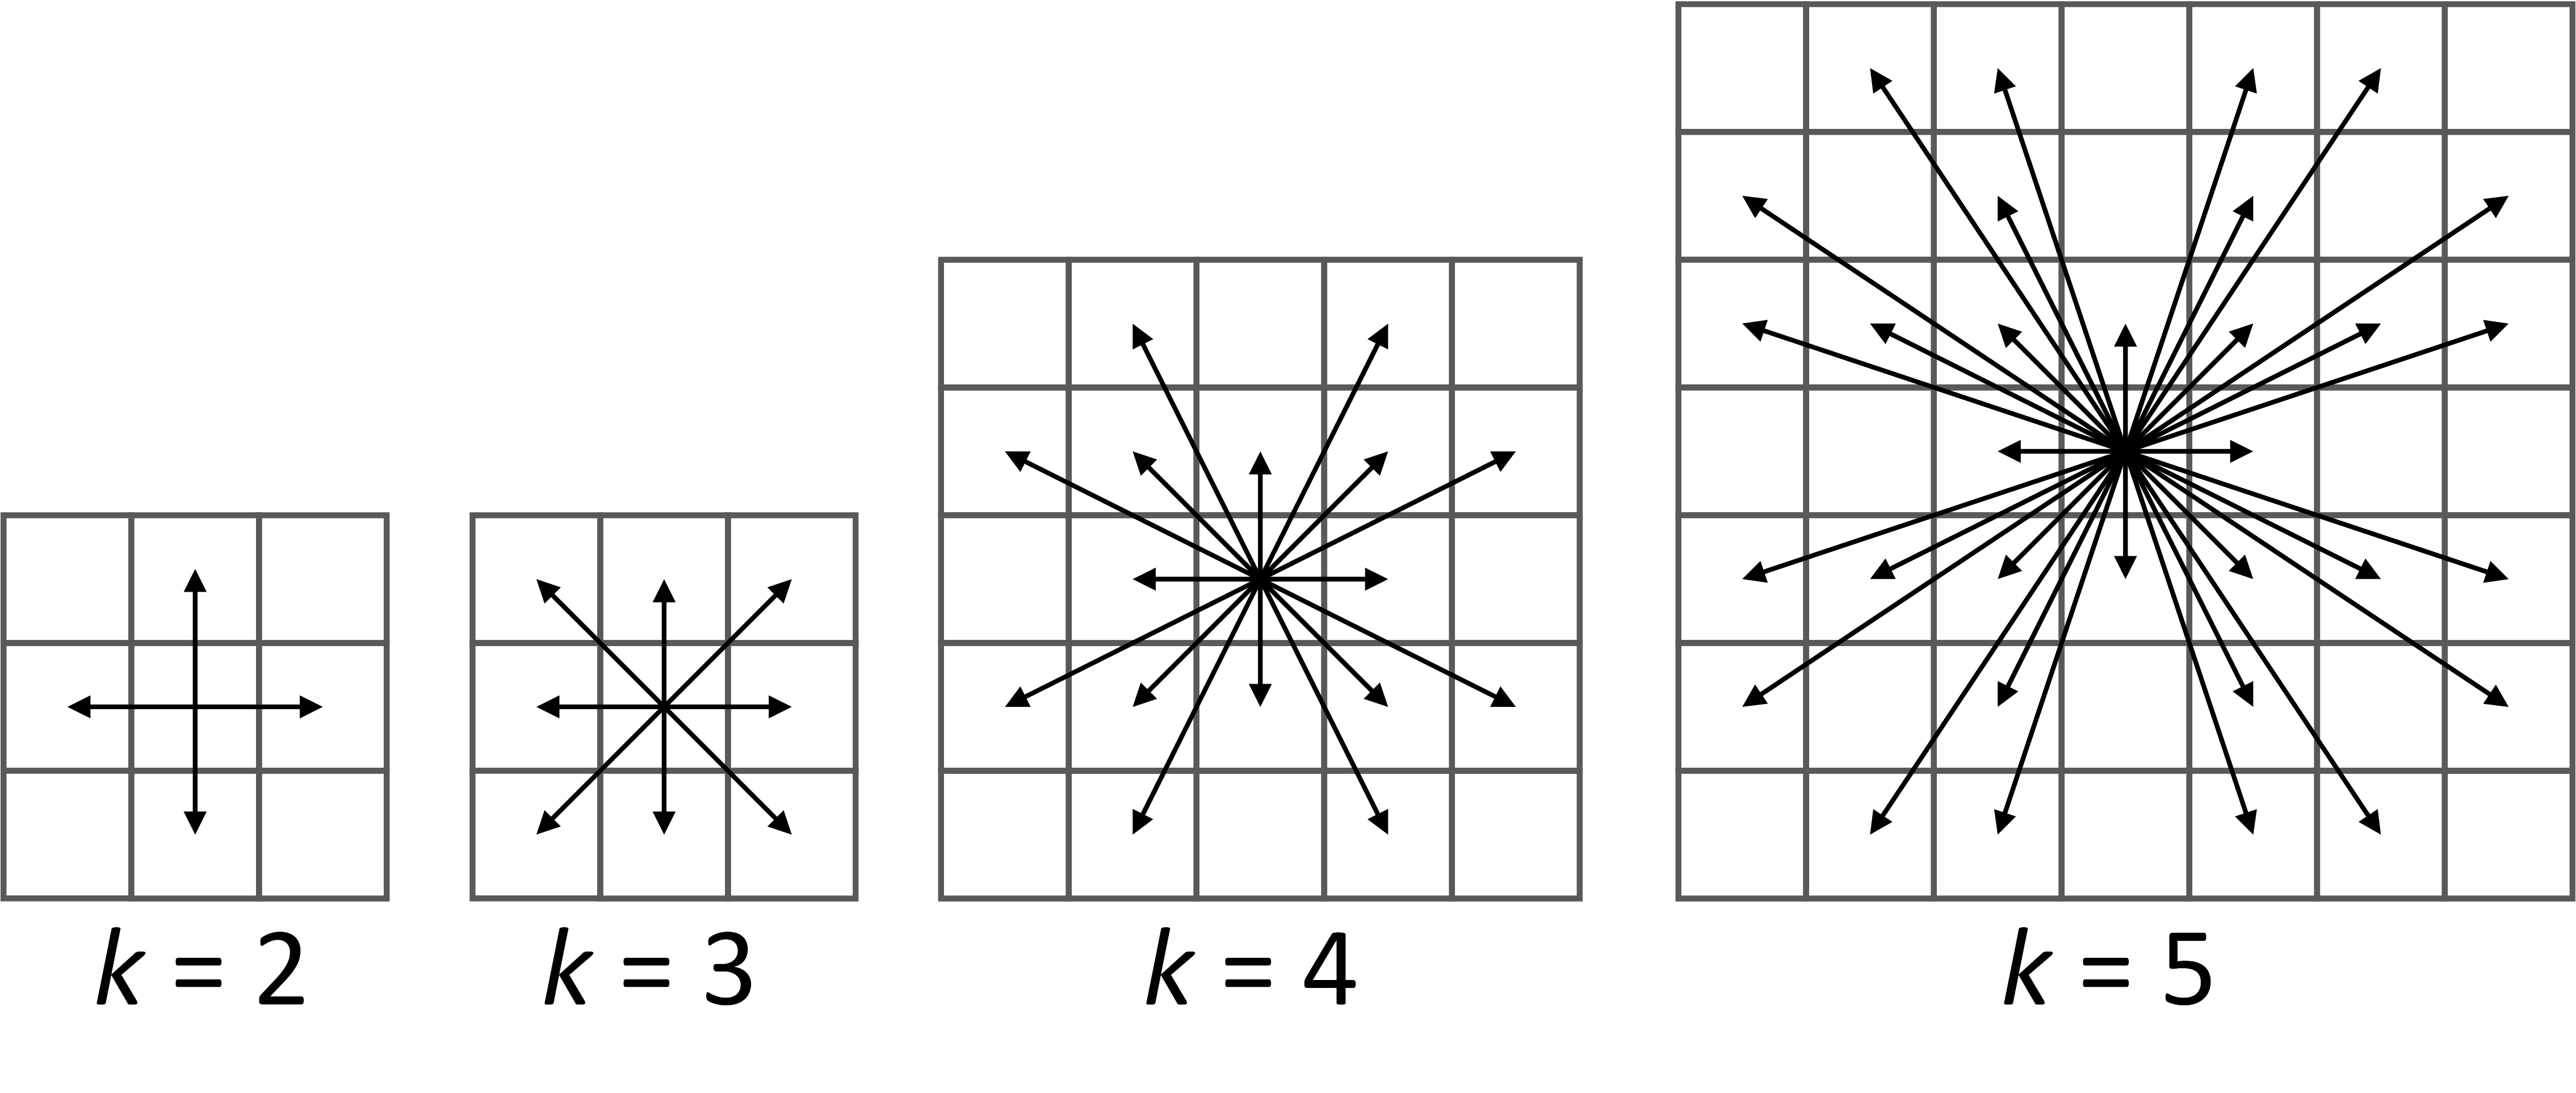
\includegraphics[width=0.75\columnwidth]{2k-neighborhood.png}
    \caption{Illustration of the $2^k$ neighborhood for $k=2,3,4,$ and $5$.}
    \label{fig:2k-grids}
\end{figure}

For each grid we set the connectivity to be $2^k$ where $k$ varied from $2$ to $5$ (see Fig.\ref{fig:2k-grids}). We assumed the moving speed of an agent (with inertial effects neglected) to be 1 grid cell per 1 time unit, that is in one time unit agent covers the segment which length is equal to the distance between two orthogonally adjacent cells. E.g. the time needed to execute a diagonal move equals $\sqrt{2}$. This time, as said before, is the cost of the corresponding \mapfr action. Agents' shapes were assumed to be disks of radius $ \frac{\sqrt{2}}{4}$. This specific size was chosen as this is the maximal size when disk agents with volume can both simultaneously perform a manoeuvre, shown in Fig.~\ref{}, that is somewhat common in classical \mapf. \konstantin{Not sure how to explain this in elegant way}.

Shape of an agent was indeed taken into account when estimating the validity of the move action w.r.t static obstacles, i.e. blocked grid cells. If the endpoints of the segment representing a move action were the centers of the free cells but the disk that moves along this segment intersects any of the blocked cells, the action was considered to be invalid.

The instances for each map were created using the \texttt{random} scenarios from \url{https://movingai.com/benchmarks/mapf.html}. There are 25 different scenarios in the set and each scenario is a list of randomly picked start-goal locations. We used this list to create instances in the way suggested by the maintainers of the benchmark repository. I.e. we started with one agent on a map and sequentially added one agent at a time by taking next start-goal pair from the scenario file, until an algorithm was not able to solve a problem in a given time limit. The latter was set to be 30 seconds. Overall, for each map and specific number of agents we ran algorithms on 25 different instances.

We also evaluated the algorithms on three different roadmaps -- \texttt{r-sparse}, \texttt{r-semi-sparse}, \texttt{r-dense} -- that were generated by processing the \texttt{den520d} map with the roadmap-generation tool used in the robotics community -- \textbf{TODO: add name and link}. The roadmaps differ in their sizes: \texttt{r-sparse} encounter XXX vertices and YYY edges, \texttt{r-semi-sparse} -- XXX vertices and YYY edges, \texttt{r-dense} -- XXX vertices and YYY edges.

Instances for the roadmaps were generated in a similar way as for grid maps. First, we generated 25 scenarios that contain non-overlapping start-goal pairs chosen randomly out of graph vertices. Then we again started with one agent on a map and sequentially added one agent at a time by taking next start-goal pair from the scenario until an algorithm was not able to solve a problem in a 30 seconds time limit.


\subsection{Design choices and implementation details}
One of the major design choice one have to make when implementing an algorithm of the \cbs family is what conflict to choose for the resolution at each iteration of high level search. Previous research on this topic in classical \mapf \cite{} \konstantin{Guys, help me with the right links} provides a clear evidence  choosing the conflicts in a right way may significantly reduce the number of nodes explored at the high level of \cbs and speed up the algorithm up to one order of magnitude or higher \konstantin{Am i not exaggerating?}. One of the common approaches to choosing conflicts that leads to such results in practice is preferring \emph{cardinal} conflicts to \emph{semi-cardinal} and preferring the latter to the \emph{non-cardinal} ones. The conflict between two plans is called cardinal if after imposing constraints and re-planning the cost of both individual plans does increase. The conflict is semi-cardinal if the cost of only one plan increases. In all other cases the conflict is non-cardinal.

Preferring cardinal conflicts to semi-cardinal to non-cardinal showed to work well for \mapfr as well. However, in \ccbs the computational cost of identifying to which class a \ccbs conflict belongs is, presumably, higher than for \cbs as now ... \textbf{TODO: add the arguments why it is true}. In our previous work \cite{andreychuk2019multi} we tried to avoid these computations in cases that heuristically seem no-promising. Nevertheless, after conducting more thorough evaluation we came to a conclusion that such an elective avoidance does not lead to a desired result (lowering down the number nodes explored at the high level) in a range of cases. Thus, we finally chose to always detect whether the newly encountered conflicts are cardinal, semi-cardinal or non-cardinal and prefer the former to the latter.

\textbf{TODO: Add implementation details of conflicts bookkeping. And a phrase on how \inconflict was implement and unsafe-intervals were computed.}

\konstantin{Pavel, do we need to say smth. about SMT-CBS?}

\subsection{Results}
Results will go here.


TODO: Anton

% START COPY AND PASTE FROM WORKSHOP PAPER



% Setting: we took grid-based setting
We conducted experiments on grids, where agents can move from the center of one grid cell 
to the center of another grid cell. 
The size of every cell is $1\times 1$, and 
the shape of every agent is a an open disk which radius equals $\sqrt{2}/4$. This specific value was chosen to allow comparison with \cbs, since it is the maximal radius that allows agents to safely perform moves in which agents follow each other.
%\footnote{In particular, this is the largest agent radius that allows the following pair of actions: agent $i$ goes up from cell $X$ to cell $Y$, and at the same time agent $j$ moves to $X$ from the right. While such train-like movements are not allowed by some \ac{MAPF} variants, they are assumed to be valid in most in research on \cbs.}




% The 2^k neighborhood
To allow non-unit edge costs, we allowed agents to move in a single move action to every cell located in their $2^k$ neighborhood, where $k$ is a parameter~\cite{rivera2017grid}. Moving from one cell to the other is only allowed if the agent can move safely to the goal cell without colliding with other agents or obstacles, where the geometry of the agents and obstacles are considered. The cost of a move corresponds to the Euclidean distance between the grid cells centers.  Figure~\ref{fig:2k} illustrates such a $2^k$ neighborhood. Increasing $k$ means a search space with higher branching factor, but also allows finding lower cost plans. 
%\roni{Maybe this is vague?} 
%As a heuristics, we pre-computed the all-pairs shortest-path distance between every pair of locations in the map, which is a perfect heuristic for single agent search. \roni{Removed for space constraints}


\subsection{Open Grids}
% First setup: open 10x10 grids, varying values of $k$
% Please add the following required packages to your document preamble:
% \usepackage{booktabs}
\begin{table}
\centering
\resizebox{0.8\columnwidth}{!}{
\begin{tabular}{@{}c|cccc|cccc@{}}
\toprule
   & \multicolumn{4}{|c}{\ac{SOC}}   & \multicolumn{4}{|c}{Success Rate} \\ \midrule
$k$ & 2     & 3    & 4    & 5    & 2    & 3    & 4    & 5    \\ \midrule
4      & 25.7  & 21.2 & 20.4 & 20.3 & 1.00 & 1.00 & 0.97 & 0.95 \\
%5      & 31.7  & 26.2 & 25.3 & 25.1 & 0.99 & 1.00 & 0.92 & 0.90 \\
6      & 38.2  & 31.6 & 30.5 & 30.2 & 0.99 & 1.00 & 0.88 & 0.83 \\
%7      & 43.8  & 36.2 & 35.0 & 34.7 & 0.98 & 0.98 & 0.84 & 0.70 \\
8      & 49.2  & 40.7 & 39.3 & 39.0 & 0.98 & 0.97 & 0.74 & 0.57 \\
%9      & 55.0  & 45.5 & 43.9 & 43.5 & 0.98 & 0.97 & 0.61 & 0.50 \\
10     & 61.0  & 50.5 & 48.8 & 48.4 & 0.95 & 0.94 & 0.54 & 0.42 \\
%11     & 68.7  & 56.8 & 54.9 & -  & 0.95 & 0.88 & 0.43 & - \\
12     & 78.0  & 64.7 & -  & -  & 0.94 & 0.86 & - & - \\
%13     & 84.6  & 70.2 & -  & -  & 0.92 & 0.76 & - & - \\
14     & 90.8  & 75.3 & -  & -  & 0.88 & 0.64 & - & -  \\
%15     & 97.1  & 80.7 & -  & -  & 0.82 & 0.58 & -  & -  \\
16     & 102.4 & 85.2 & -  & -  & 0.76 & 0.53 & -  & -  \\
%17     & 108.3 & 90.4 & -  & -  & 0.71 & 0.42 & -  & -  \\
18     & 118.7 & -  & -  & -  & 0.62 & - & -  & -  \\
%19     & 125.5 & -  & -  & -  & 0.56 & -  & -  & -  \\
20     & 131.7 & -  & -  & -  & 0.46 & -  & -  & - \\\bottomrule
\end{tabular}
}
\caption{Results for \ccbs on $10\times 10$ open grid.}% for $k=2, 3, 4$, and $5$}
\label{tab:10x10}
\vspace{-0.3cm}
\end{table}

\commentout{
\begin{table}
\resizebox{\columnwidth}{!}{
\begin{tabular}{@{}c|cccc|cccc@{}}
\toprule
   & \multicolumn{4}{|c}{\ac{SOC}}   & \multicolumn{4}{|c}{Success Rate} \\ \midrule
$k$ & 2     & 3    & 4    & 5    & 2    & 3    & 4    & 5    \\ \midrule
4      & 25.7  & 21.2 & 20.4 & 20.3 & 1.00 & 1.00 & 0.97 & 0.95 \\
5      & 31.7  & 26.2 & 25.3 & 25.1 & 0.99 & 1.00 & 0.92 & 0.90 \\
6      & 38.2  & 31.6 & 30.5 & 30.2 & 0.99 & 1.00 & 0.88 & 0.83 \\
7      & 43.8  & 36.2 & 35.0 & 34.7 & 0.98 & 0.98 & 0.84 & 0.70 \\
8      & 49.2  & 40.7 & 39.3 & 39.0 & 0.98 & 0.97 & 0.74 & 0.57 \\
9      & 55.0  & 45.5 & 43.9 & 43.5 & 0.98 & 0.97 & 0.61 & 0.50 \\
10     & 61.0  & 50.5 & 48.8 & 48.4 & 0.95 & 0.94 & 0.54 & 0.42 \\
11     & 68.7  & 56.8 & 54.9 & -  & 0.95 & 0.88 & 0.43 & 0.31 \\
12     & 78.0  & 64.7 & -  & -  & 0.94 & 0.86 & 0.32 & 0.24 \\
13     & 84.6  & 70.2 & -  & -  & 0.92 & 0.76 & 0.22 & 0.15 \\
14     & 90.8  & 75.3 & -  & -  & 0.88 & 0.64 & 0.18 & -  \\
15     & 97.1  & 80.7 & -  & -  & 0.82 & 0.58 & -  & -  \\
16     & 102.4 & 85.2 & -  & -  & 0.76 & 0.53 & -  & -  \\
17     & 108.3 & 90.4 & -  & -  & 0.71 & 0.42 & -  & -  \\
18     & 118.7 & -  & -  & -  & 0.62 & 0.32 & -  & -  \\
19     & 125.5 & -  & -  & -  & 0.56 & -  & -  & -  \\
20     & 131.7 & -  & -  & -  & 0.46 & -  & -  & - \\\bottomrule
\end{tabular}
}
\caption{Results for \ccbs on $10\times 10$ open grid.}% for $k=2, 3, 4$, and $5$}
\label{tab:10x10}
\end{table}
}

For the first set of experiments we used a
$10\times 10$ open grid, placing agents' start and goal locations randomly. We run experiments with 4, 5, $\ldots, 20$ agents. For every number of agents we created 250 different problems. 
Each problem was solved with \ccbs with $k=2, 3, 4$, and $5$. 
%\roni{TODO: Add supp.} 
An animation of a solution found by \ccbs for a problem with 13 agents and different values of $k$ can be seen in \url{https://tinyurl.com/ccbs-example}.
%The file \texttt{CCBS.mp4} in the supplementary material shows an animation of the solution found by \ccbs for a problem with 13 agents and different values of $k$. 
Table~\ref{tab:10x10} shows the results of this set of experiments. 
 Every row shows results for a different number of agents, 
as indicated on the left-most column. 
The four right-most columns show the success rate, i.e., the ratio of problems solved by the \ccbs under a timeout of 60 %\roni{Anton what was the timeout?} 
seconds, out of a total of 250 problems. 
Data points marked by ``-'' indicate settings where the success rate was lower than 0.4. The next four columns show the average \ac{SOC}, 
averaged over the problems solved by all \ccbs instances that had a success rate larger than 0.4. 

%\roni{Was this the cutoff?} \textbf{K: Actually the cut-off was "lower than 50\%", but Anton continued running the experiments when it was not super time-consuming. That is why we have some extra data points.}

The results show that increasing $k$ yields solutions with lower \ac{SOC}, as expected. 
The absolute difference in \ac{SOC} when moving from $k=2$ to $k=3$ is the largest, and it grows as we add more agents. For example, for problems with 14 agents, moving from $k=2$ to $k=3$ yields an improvement of 15.5 \ac{SOC}, 
and for problems with 16 agents the gain of moving to $k=3$ is 17.2 \ac{SOC}. Increasing $k$ further exhibits a diminishing return effect, where the largest average \ac{SOC} gain when moving from $k=4$ to $k=5$ is at 0.5. 
%\roni{Maybe bla a bit on why this is, although I think it is obvious.} 



Increasing $k$, however, has also the effect of increasing the branching factor, which in turns means that path-finding becomes harder. Indeed, the success rate of $k=5$ is significantly lower compared to $k=4$. An exception to this is the transition from $k=2$ to $k=3$, where we observed a slight advantage in success rate for $k=3$ for problems with a small number of agents. For example, with 6 agents the success rate of $k=2$ is 0.99 while it is 1.00 for $k=3$. An explanation for this is that increasing $k$ also means that plans for each agent can be shorter, which helps to speedup the search. Thus, increasing $k$ introduces a tradeoff w.r.t. the problem-solving difficulty: the resulting search space for the low-level search is shallower but wider. For denser problems, i.e., with more agents, $k=2$ is again better in terms of success rate, as more involved plans must be found by the low-level search. 

\commentout{
\begin{figure}
    \centering
    \includegraphics[width=\columnwidth]{soc-gain.PNG}
    \caption{10$\times$10 open grid, gain of using \ccbs over  \cbs.}
    \label{fig:soc-gain}
\end{figure}
Figure~\ref{fig:soc-gain} shows the tradeoff of increasing $k$ by showing the average \emph{gain}, in terms of \ac{SOC}, of using \ccbs for different values of $k$
over \ccbs with $k=2$. The $x$-axis is the number of agents, and the $y$-axis is the gain, in percentage. We only provide data points for configurations with a success rate of at least 40\%. As can be seen, increasing $k$ increases the gain over \cbs, where for $k=4$ and $k=5$ the gain was over 20\%. Increasing $k$ also decreases the success rate, and thus the data series for larger $k$ value ``disappears'' after a smaller number of agents. 
}

\begin{figure}
    \centering
    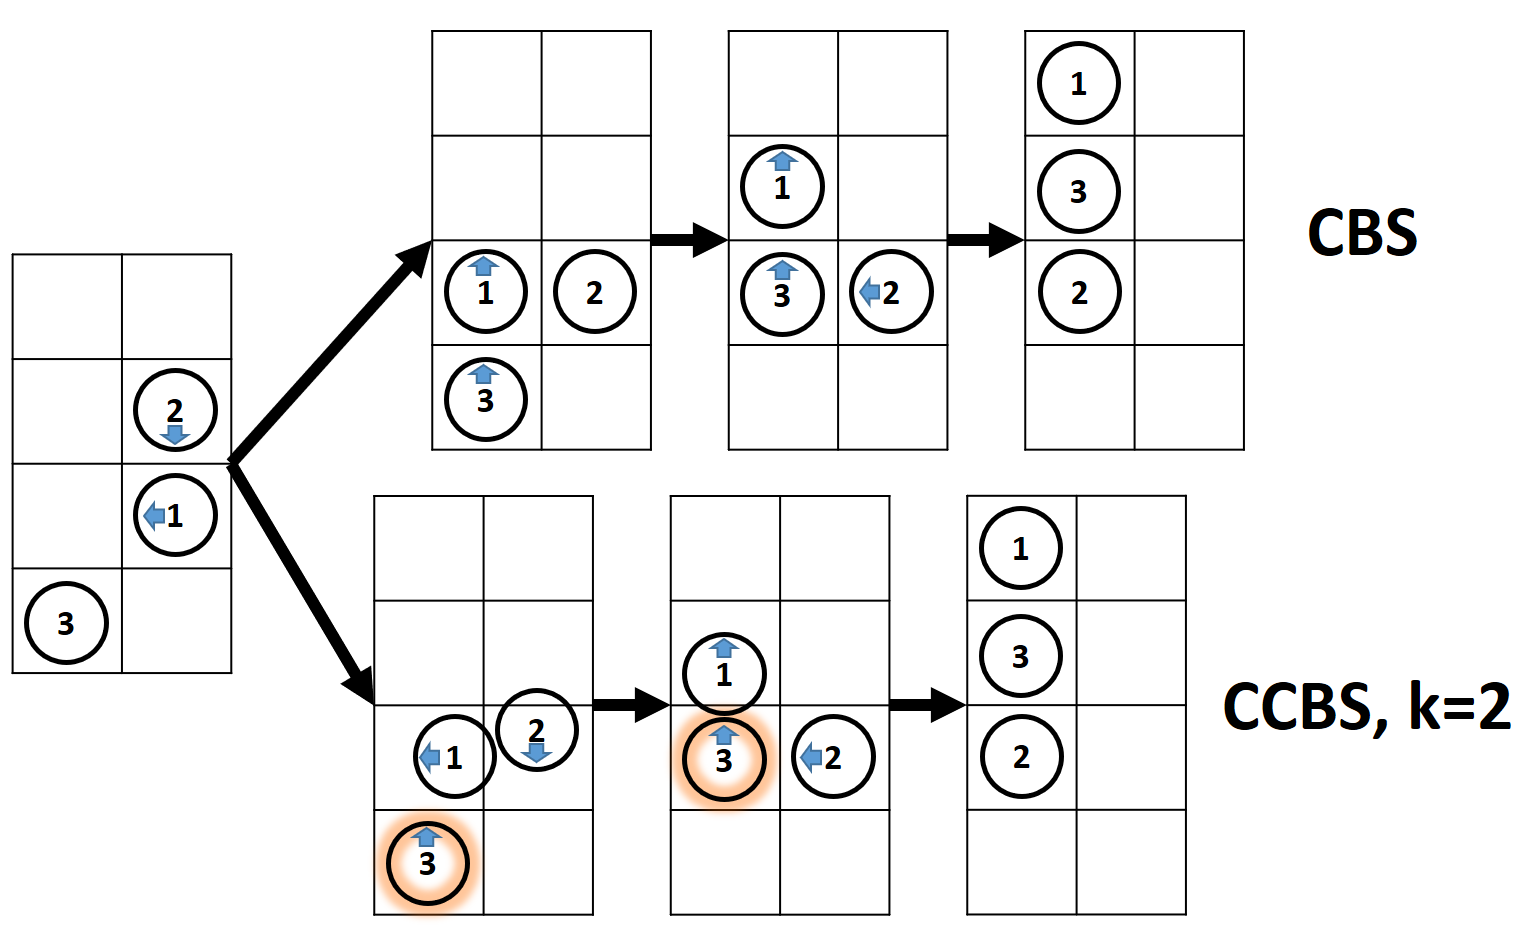
\includegraphics[width=0.7\columnwidth]{anton-example.PNG}
    \caption{Example: \ccbs for $k=2$ finds better  solution than \cbs.}
    \label{fig:anton-example}
\end{figure}

% Something about the standard CBS
We also compared the performance of \ccbs with $k=2$ and a standard \cbs implementation. 
\cbs was faster than \ccbs, as its underlying solver is \astar on a 4-connected grid, 
detecting collisions is trivial, and it has only unit-time wait actions. However, even for $k=2$, \ccbs is able to find better solutions, i.e., solutions of lower \ac{SOC}. This is because, an agent may start to move after waiting less than a unit time step. 
Figure~\ref{fig:anton-example} illustrates such a scenario. An animation of this example is given in \url{https://tinyurl.com/ccbs-vs-cbs2}. %file \texttt{C-CBSvsCBS.gif} in the supplementary material. % shows an animation of this example. 


%To see this phenomenon, consider the example in Figure~\ref{fig:anton-example}. There are three agents, 1,2, and 3 in an open 2$\times$4 grid.  The left-most grid shows the initial locations of the agents,  and the right-most grid shows their goal locations. The small arrows in the agents indicate the direction each agent is about to move to.  Consider first the plan created by \cbs, which is shown on the top row of Figure~\ref{fig:anton-example}. In \cbs,  every action takes unit duration. Since agent 3 cannot move upwards at time $t=0$ without colliding with agent 1, it will have to wait for time $t=1$ before starting to move.  By contrast, in \ccbs a wait action can have an arbitrary duration, and thus agent 3 can start to move upwards safely earlier than in \cbs, at time $t=0.707$. See the file \texttt{C-CBSvsCBS.gif} in the supplementary material for an animation of this example. These cases, where \ccbs with $k=2$ finds a better solution compared to standard \cbs, are not rare. However, the advantage in terms of \ac{SOC}, in all our experiments, was very small. 




\subsection{Dragon Age Maps}
%\begin{figure}
%    \centering
%    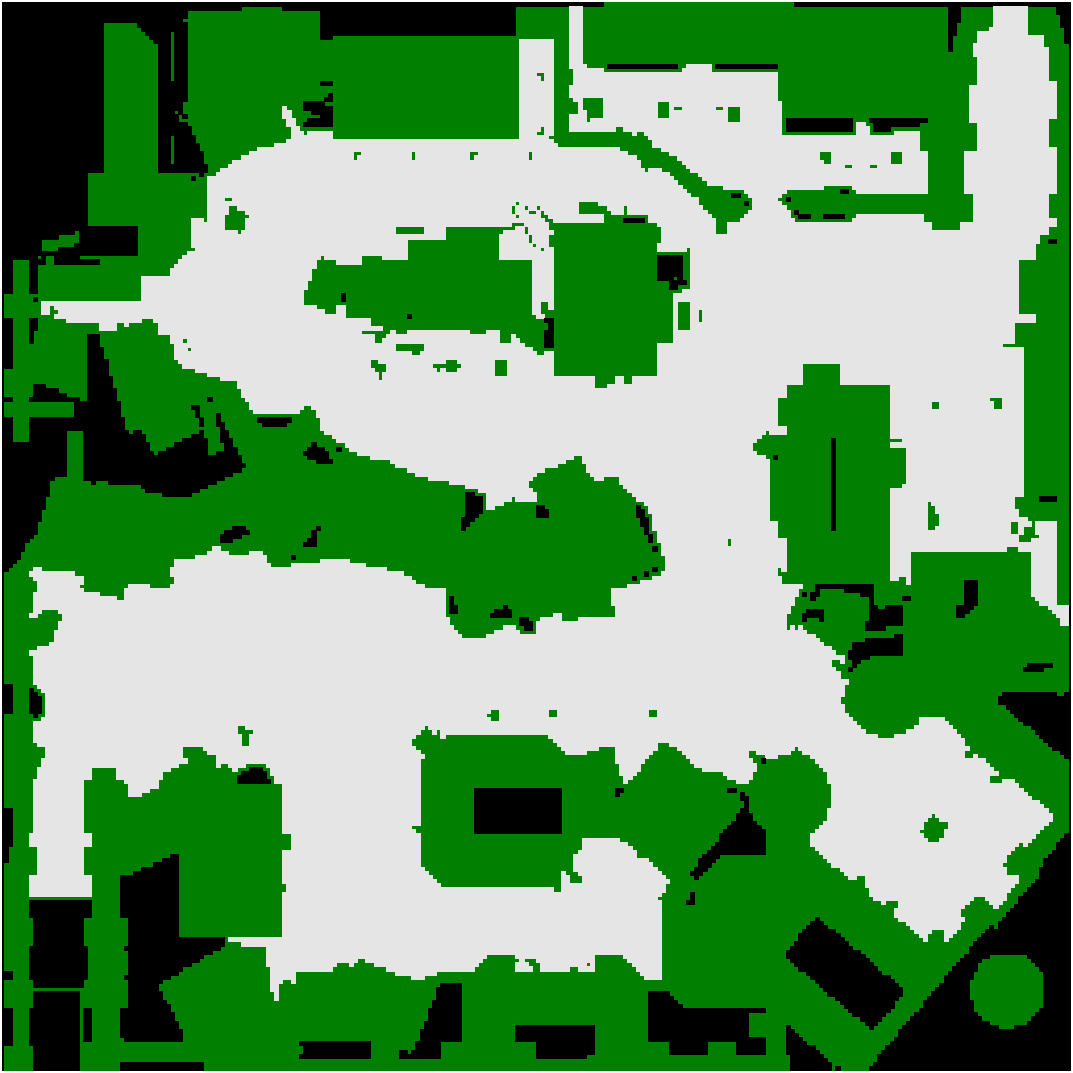
\includegraphics[width=0.5\columnwidth]{den520d.png}
%    \caption{The \texttt{den520d} DAO map used in our experiments. \roni{Add some more figures near by to save space.}}
%    \label{fig:dao}
%\end{figure}


% Please add the following required packages to your document preamble:
% \usepackage{booktabs}
\begin{table}
\centering
\resizebox{0.7\columnwidth}{!}{
    \begin{tabular}{@{}c|ccc|ccc@{}}
    \toprule
    \multicolumn{1}{l|}{} & \multicolumn{3}{c|}{\ac{SOC}} & \multicolumn{3}{c}{Success Rate} \\ \midrule
    k                     & 2      & 3      & 4      & 2         & 3         & 4        \\ \midrule
    10                    & 1,791  & 1,515  & 1,460  & 0.96      & 0.93      & 0.86     \\
    15                    & 2,598  & 2,198  & 2,118  & 0.94      & 0.84      & 0.70     \\
    20                    & 3,347  & 2,829  & 2,726  & 0.79      & 0.72      & 0.50     \\
    25                    & 4,049  & 3,426  & 3,304  & 0.58      & 0.58      & 0.32     \\ \bottomrule
    \end{tabular}
}
$\vcenter{\hbox{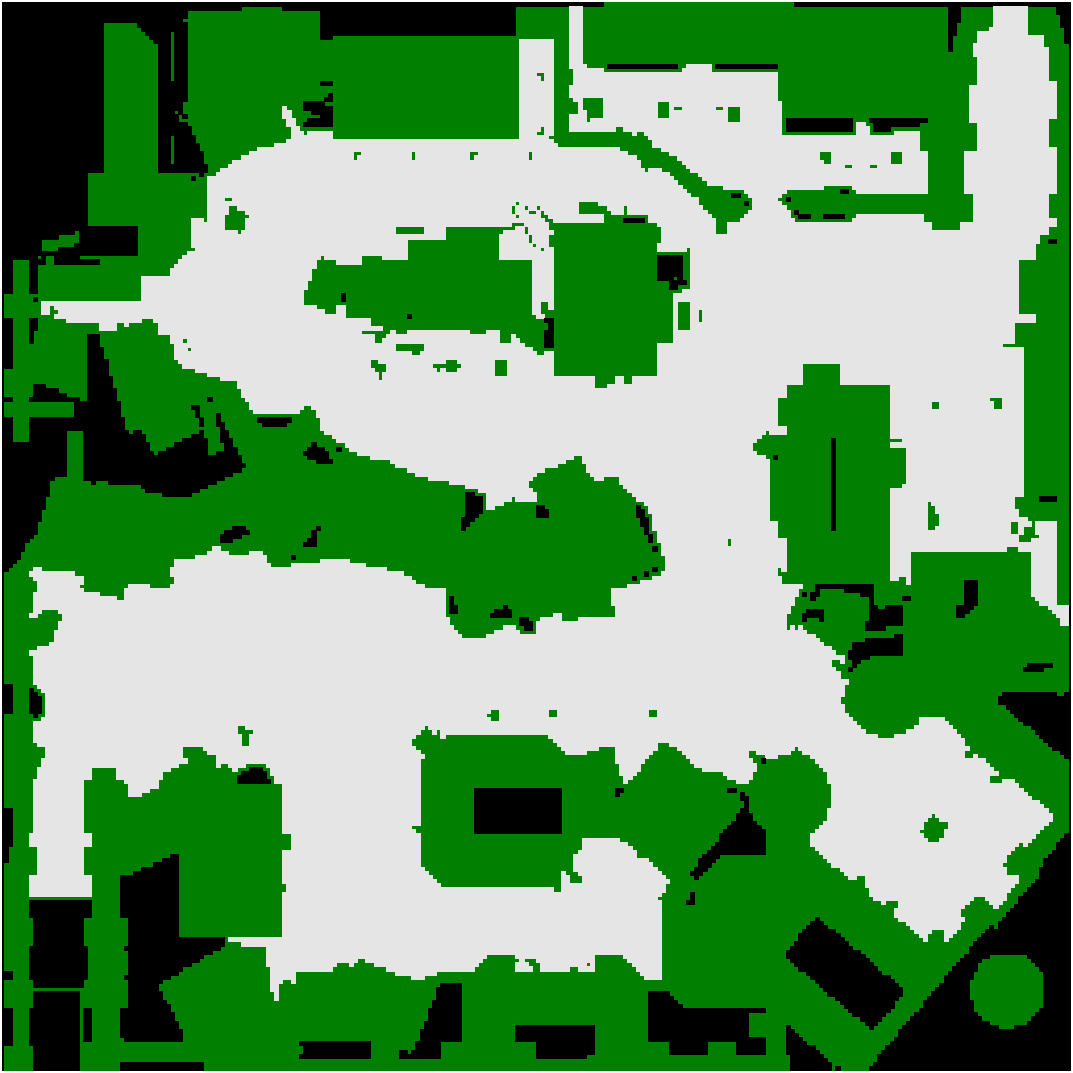
\includegraphics[width=0.25\columnwidth]{den520d.png}}}$
    %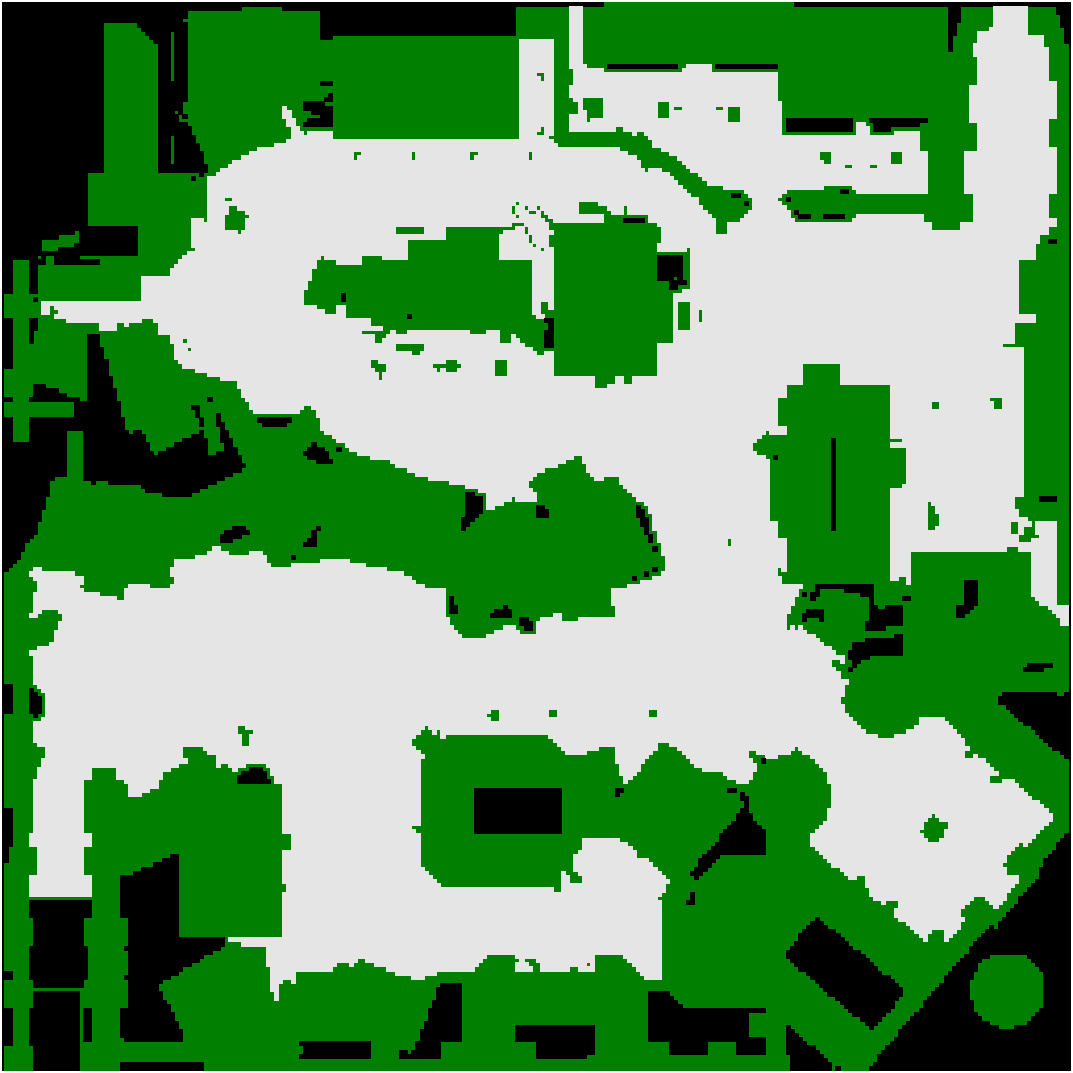
\includegraphics[width=0.25\columnwidth]{den520d.png}

\caption{Results for \ccbs on the \texttt{den520d} DAO map.}
\label{tab:dao}
\vspace{-0.3cm}
\end{table}

% Different k values DAO
Next, we experimented with a larger grid, taken from the Dragon Age: Origin (DAO) game and made available in the \texttt{movingai} repository~\cite{sturtevant2012benchmarks}. We used the \texttt{den520d} map, shown to the right of Table~\ref{tab:dao}, which was used by prior work~\cite{sharon2015conflict}. 
Start and goal states were chosen randomly, and we create 250 problems for every number of agents.
%\roni{Anton: did you choose start and goal randomly, or using some other method?}Anton: yes, randomly
\commentout{
\begin{figure}
    \centering
    \includegraphics[width=\columnwidth]{runtime-dao_cropped.pdf}
    \caption{The average runtime for the DAO map.}
    \label{fig:dao-runtime}
\end{figure}
}
Table~\ref{tab:dao} shows the results obtained for \ccbs with $k=2,3,$ and $4$, 
in the same format as Table~\ref{tab:10x10}. The same overall trends are observed: increasing $k$ reduces the SOC and decreases the success rate. %Figure~\ref{fig:dao-runtime} shows the  average runtime required to solve the instances solved by all values of $k$. Interestingly, here we observe that $k=3$ was the fastest on average. Similar to the better success rate in the open grid experiments, we explain this by the fact that increasing $k$ also yields shorter paths to the goals, which helps decrease runtime. %This behavior corresponds to the results reported in the previous set of experiments. observed for the open gri

%\roni{Maybe put here the roadmap experiments?}


\subsection{Conflict Detection and Resolution Heuristics}


% Please add the following required packages to your document preamble:
% \usepackage{booktabs}

\begin{table}
\centering
\resizebox{0.9\columnwidth}{!}
{
\begin{tabular}{@{}lrrrrr@{}}
\toprule
  & &\multicolumn{1}{c}{Vanilla} & \multicolumn{1}{c}{PastConf} & \multicolumn{1}{c}{Cardinals} & \multicolumn{1}{c}{Hybrid} \\ \midrule

%\multirow{3}{*}{\begin{sideways}20 agents\end{sideways}} & \multirow{3}{*}{\begin{sideways}$k$=2\end{sideways}} & Succ.     & 0.72   & 0.74 & 0.75 & 0.82\\
\multirow{2}{*}{
\parbox{1.5cm}{$k$=2 Agents=20}} & Success     & 0.72   & 0.74 & 0.75 & 0.82         \\
%& Time     & 4.57   & 3.55 & 5.86 & 2.16                      \\
& HL exp. & 765    & 712 & 453 & 452                    \\ \midrule
\multirow{2}{*}{\parbox{1.5cm}{$k$=3 Agents=20}} & Success     & 0.67   & 0.68    & 0.75      & 0.76   \\
%& Time     & 1.83   & 1.65    & 1.70      & 1.51   \\
& HL exp.  & 152    & 141     & 51        & 47     \\ \midrule
\multirow{2}{*}{\parbox{1.5cm}{$k$=4 Agents=20}} & Success     & 0.39   & 0.4    & 0.48      & 0.50   \\
%& Time     & 4.67   & 3.84    & 3.83      & 2.71   \\
& HL exp.  & 564    & 516     & 232       & 270     \\ \midrule
\multirow{2}{*}{\parbox{1.5cm}{$k$=2 Agents=25}} & Success  & 0.39   & 0.43    & 0.38      & 0.53   \\
%& Time     & 10.25  & 7.33   & 13.08    & 3.66  \\
& HL exp. & 1762   & 1730    & 968       & 990  \\ \midrule
\multirow{2}{*}{\parbox{1.5cm}{$k$=3 Agents=25}} & Success  & 0.44   & 0.45    & 0.60      & 0.61   \\
%& Time     & 3.32  & 2.74   & 2.88    & 2.34  \\
& HL exp. & 313   & 270   & 81       & 72  \\ \bottomrule

\end{tabular}
}
\caption{Comparing conflict detection and selection methods.}
\label{tab:heuristics}
\end{table}

%\multirow{-10}{*}{\cellcolor{yellow}\begin{sideways}TEST\end{sideways}}%

In all the experiments so far we have used \ccbs with the hybrid conflict detection and selection heuristic described earlier in the paper. Here, we evaluate the benefit of using this heuristic. We compared \ccbs with this heuristic against the following: (1) Vanilla: \ccbs that chooses arbitrarily which actions to check first for conflicts, 
(2) Cardinals: \ccbs that identifies all conflicts and chooses cardinal conflicts,   
and (3) PastConf: \ccbs that uses the \history heuristic to choose where to search for conflicts first, and resolves the first conflict it finds.  

%Table~\ref{tab:heuristics} shows results for experiments run on the \texttt{den520d} DAO map.
Table~\ref{tab:heuristics} shows results for the \texttt{den520d} DAO map for 20 agents with $k=$ 2, 3, and 4; and 25 agents with $k$=2 and $k$=3. For every configuration we create and run \ccbs on 1,000 instances. The table shows the success rate (the row labelled ``Success'')  
%the average runtime in seconds over instances solved by all algorithms (``Time''), 
and the average number of high-level nodes expanded by \ccbs (``HL exp.''). The results show that the proposed hybrid heuristic 
enjoys the complementary benefits of PastConf and Cardinals, 
expanding as few \ct nodes as Cardinals 
and having the highest success rate. %, expanding as few \ct nodes as Cardinals and enjoys the complementary benefits of PastConf and Cardinals: , as can be seen by its high success rate and small number of high-level expanded nodes. Thus, we used it in all our experiments. 

%When comparing PastConf to Cardinals, we see that PastConf has a higher success rate but the number of high-level nodes expanded by Cardinals is smaller. This follows our motivation for the hybrid heuristic: the choice of which conflicts to resolve taken by Cardinals is important in minimizing the size of the CT, while detecting all conflicts can be too time consuming. The proposed hybrid heuristic enjoys the complementary benefits of PastConf and Cardinals, as can be seen by its high success rate and small number of high-level expanded nodes. Thus, we used it in all our experiments. 
%its fast runtime and small number of high-level expanded nodes. Thus, we used it in all our experiments. 

\subsection{Comparison to E-ICTS}


\begin{figure}
    \centering
    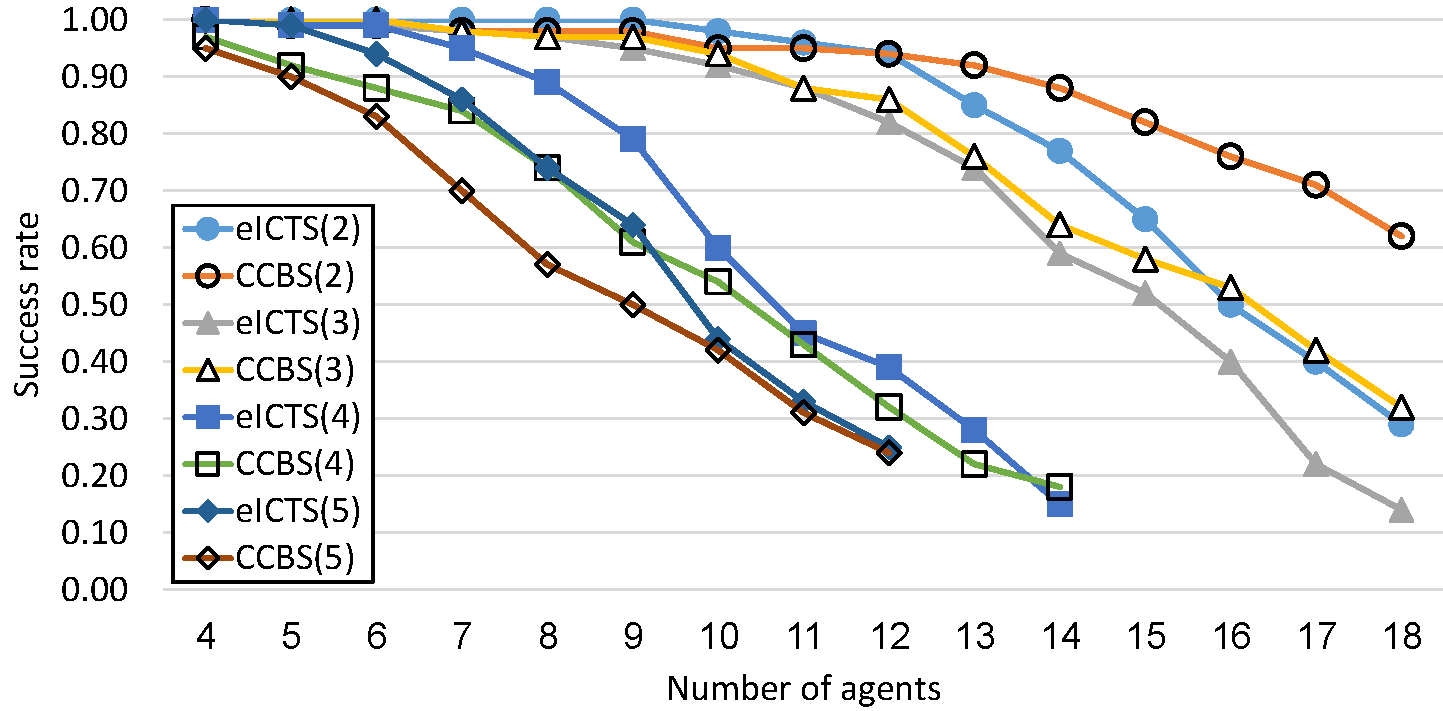
\includegraphics[width=0.85\columnwidth]{ccbsVsICTS_cropped.pdf}
    %\includegraphics[width=0.30\columnwidth]{roadmap_cropped.pdf}
    \caption{Success rate of \ccbs and E-ICTS in 10$\times$10 open grids.}
    \label{fig:ccbs-vs-eicts}
    \vspace{-0.3cm}
\end{figure}


Finally, we compared the performance of \ccbs and E-ICTS~\cite{walker2018extended}, a \mapfr algorithm based on the Increasing Cost Tree Search (ICTS) framework~\cite{sharon2013increasing}. Like \ccbs, E-ICTS 
can also handle non-unit edge cost. 
E-ICTS handles continuous time by discretizing it according to a minimal wait time parameter $\Delta$. 
Figure~\ref{fig:ccbs-vs-eicts} shows the success rate of the two algorithms on open $10\times10$ grids with different number of agents and $k=2, 3, 4,$ and 5. 
We thank the E-ICTS authors who made their implementation publicly available (\url{https://github.com/nathansttt/hog2}). 


The results show that for $k=2$ and $k=3$, \ccbs works better in most cases, while E-ICTS outperforms \ccbs for $k=4$ and $k=5$. The reason for this is that as $k$ increases, more actions conflict with each other, resulting in a significantly larger \ct. Developing pruning techniques for such \ct is a topic for future work. We also compared \ccbs to ICTS over larger dragon age maps. The results where that in most cases E-ICTS solved more instances. 

%In all cases, \ccbs founds a solution that is either the same or slightly better than E-ICTS. This is because  \ccbs handles continuous time directly while E-ICTS discretizes it. 

Note that given an accurate unsafe interval detection mechanism, \ccbs handles continuous time directly, and thus can return better solutions than E-ICTS. However, the unsafe interval detection mechanism we implemented did, in fact, discretize time, and so the comparison to E-ICTS is valid. That being said, we note that these are different implementations and different algorithmic families, and we do not presume to infer from this set of experiments when each algorithm is better. This is an open question even for basic \mapf.  

\commentout{
\begin{figure}
    \centering
    \includegraphics[width=0.35\columnwidth]{roadmap_cropped.pdf}
    \caption{The roadmap created for \texttt{den520d} DAO map.}
    \label{fig:roadmap}
\end{figure}
}
We also performed a limited set of experiments on roadmaps, to demonstrate the applicability of \ccbs beyond grid domains. 
%We created roadmaps  based on the the \texttt{den520d} DAO map using the OMPL library (http://ompl.kavrakilab.org), which is a widely used robotics library for path planning.
%Figure~\ref{fig:roadmap} shows a roadmap 
We created a roadmap with 878 vertices and 14,628 edges based on the \texttt{den520d} DAO map using the OMPL library (http://ompl.kavrakilab.org). 
%, which is a widely used robotics library for path planning. 
We create 250 problems with 10, 15, and 20 agents. The resulting success rate was 0.89, 0.60, and 0.22, 
and the SOC was 1,459, 2,082, and 2,688, respectively. 
In \url{https://tinyurl.com/ccbs-roadmap2} there is an animation showing a solution found by \ccbs for a small roadmap. 


% END COPY AND PASTE FROM WORKSHOP PAPER

\section{Related Work}
TODO: Roni

Works related to us but not needed to explain our approach


% START COPY AND PASTE FROM WORKSHOP PAPER


% Some prior work
%Several prior work considered \mapfrelax some of the simplifying assumptions made by most \ac{MAPF} research. 
Yakovlev and Andreychuk~\shortcite{yakovlev2017anyAngle} proposed AA-SIPP($m$), an any-angle \ac{MAPF} algorithm. 
%for agents  hat can move along in any angle they choose.  Their algorithm, called AA-SIPP($m$), 
AA-SIPP($m$) is based on \sipp and adopts a prioritized planning approach. Ma et al.~\shortcite{ma2019lifelong} also used \sipp in a prioritized planning framework for lifelong \mapf. Both algorithms do not guarantee completeness or optimality. 
%They too cannot guarantee optimality or completeness, and are limited to 4-connected grids.  is similar to \ccbs in that agents can wait for any desired duration. Also, AA-SIPP($m$) heavily relies on \ac{SIPP}. Unlike \ccbs, they adopted a prioritized planning approach that does not guarantee completeness or optimality.  Ma et al.~\shortcite{ma2019lifelong} used \sipp in a prioritized planning framework for lifelong \mapf. They too cannot guarantee optimality or completeness, and are limited to 4-connected grids. 
%: agents plan sequentially, and an agent is constrained to avoid conflicting with the plans already created for other agents. Consequently, AA-SIPP($m$) 
Li et al.~\shortcite{li2019multi} proposed \ac{MCCBS}, a \cbs-based algorithm for agents with a geometrical shape that may have different configuration spaces. However, they assumed all actions have a unit duration and did not address continuous time. %We note that adapting \ccbs to cases where the agents have different configuration spaces, requires no algorithmic changes.
%Li et al.~\shortcite{li2019multi} proposed a \cbs-based algorithm for solving the Large-Agents \ac{MAPF} (LA-MAPF) problem. In LA-MAPF, agents have a geometrical shape, and may have different configuration spaces. Their algorithm, called \ac{MCCBS}, is also based on \cbs.  However, they assumed all actions have a unit duration and did not address continuous time. We note that adapting \ccbs to cases where the agents have different configuration spaces, requires no algorithmic changes.  
%Walker et al.~\shortcite{walker2018extended}  adapted the \ac{ICTS} \ac{MAPF} algorithm~\cite{sharon2013increasing} to \mapfr, that is, to consider actions with non-uniform duration and agents with a geometric shape. However, their extended \ac{ICTS} does not allow agents to wait an arbitrary amount of time, and relies on discretizing the possible wait times (they called it $\delta$). By contrast, \ccbs relies on a different \ac{MAPF} framework -- \cbs -- and do not require a-priori definition of the smallest wait action. Still, \ccbs maintains optimality and completeness. 
%In a different work, 
Walker et al.~\shortcite{walker2017using} proposed \cbs-CL, a \cbs-based algorithm designed to handle non-unit edge costs and hierarchy of movement abstractions. \cbs-CL does not allow reasoning about continuous time and does not return provably optimal solutions. H{\"o}nig et al.~\shortcite{honig2017summary} proposed MAPF-POST, which is a post-processing step that adapts a \ac{MAPF} solution to different action durations that due to kinematic constraints. MAPF-POST does not guarantee optimality as well. 



dRRT* is a sample-based \ac{MAPF} algorithm designed for continuous spaces~\cite{dobson2017scalable}. dRRT* is asymptotically complete and optimal while \ccbs is optimal and complete, and is designed to run over a discrete graph. ORCA~\cite{van2005prioritized,snape2011hybrid} 
and ALAN~\cite{godoy2018alan} are fast and distributed \ac{MAPF} algorithms for continuous space, but they do not provide optimality or completeness guarantees. 



%\roni{Verify that this is correct} \roni{TODO Roni: add a bit more references to suboptimal MAPF.}\roni{Konstantin: can you add a bit about any-angle stuff for MAPF?}



Table~\ref{tab:related-work} provides an differential overview of related work on \ac{MAPF} beyond its basic setting. 
Columns ``N.U.'',  ``Cont.'', ``Ang.'', ``Vol.'', ``Opt.'', and ``Dist.'', means support for non-uniform action durations, 
actions with arbitrary continuous duration, 
actions beyond the 4 cardinal moves, agents with a volume (i.e., some geometric shape), 
returns a provably optimal solution, 
and distributed algorithm, respectively. Rows correspond to  different algorithms or family of algorithms. %The \ccbs row is highlighted. % to the generality of \ccbs. 

%Yakovlev and Andreychuk~\shortcite{yakovlev2017anyAngle} yakovlev2017anyAngle


% END COPY AND PASTE FROM WORKSHOP PAPER

%\section{Discussion}

%\subsection{Continuous Space} TODO: Konstantin \textbf{K: I don't think we need this section anymore}

%There are many ways to define what ``continuous space'' means ....


%When an agent moves it occupies an area in some time.  1) All is blocked until action is done 2) Tiles are blocked for specified discrete times 3) Space is continuos, and time is contiuos, some words that shoudl make sense???
% a) Specific vertices and edges, but agents have a shape and moving along an edge occupies ...[[some word that means space and time are continuous in this movement, not like tiles approach]]
% b) Any-angle -- agent move from vertex to vertex, but are not confined to specific edges
% c) Any-position -- there are no vertices -- agents are allowed to occupy any position in some Euclidean space Configuration space search -- instead of a location, the agent has a configuration, this includes the space it occupies, but also its orientation, % and structure (think robotic arm)


\section{Conclusion}

% START COPY AND PASTE FROM WORKSHOP PAPER


We proposed \ccbs, a sound, complete, and optimal \mapf algorithm that supports continuous time, actions with non-uniform duration, and agents and obstacles with a geometric shape. 
\ccbs follows the \cbs framework, using an adapted version of \sipp as a low-level solver, and unique types of conflicts and constraints in the high-level search. 
%We prove that \ccbs is sound, complete, and optimal. 
To the best of our knowledge, \ccbs is the first \ac{MAPF} algorithm to provide optimality guarantees for such a broad range of \ac{MAPF} settings. 
Our experimental results showed that \ccbs can solve actual \ac{MAPF} problems and finds better solutions than \cbs. Comparing to E-ICTS, \ccbs is sometimes faster and sometimes slower, but it always returns better solutions.  
%However, current results were based on grid maps that are extended by considering $2^k$ neighborhoods. We chose grids as a domain to allow natural comparison with existing solvers, but \ccbs can work on arbitrary graphs. Indeed, this is a topic for future work. 
This work also highlighted that conflict detection becomes a bottleneck when solving \mapfr problems. We suggested a hybrid heuristic for reducing this cost. Future work may apply meta-reasoning techniques to decide when and how much to invest in conflict detection throughout the search. 

%TODO: MENTION Lifelong Path Planning with Kinematic Constraints for Multi-Agent Pickup and Delivery (not CBS, but uses SIPP, computes collisions geometrically, but only for 4-connected)







% END COPY AND PASTE FROM WORKSHOP PAPER



\subsubsection*{Acknowledgments}
This research was partially funded by the ISF grant to Dr. Roni Stern no. 201/17. 

\appendix

\section{Pseudo Code for Generating the \mddr}
\label{sec:code-mddr}


\begin{algorithm}[t]
	\SetKwInOut{Input}{input}
	\Input{$\mathcal{G}=(V,E)$, \source(i), \target(i), $\mu$, \implicitct)}
	$\textsc{Open} \gets \emptyset$ \\   
	insert $(\source(i),0)$ into $\textsc{Open}$\\
	$X^i \gets \{ (\source(i),0) \}$\\
	$E^i \gets \emptyset$\\    	
	\While {$\textsc{Open} \neq \emptyset$} {
		$(v,t) \gets$ min$_{t}(\OPEN)$\\
		Remove $(v,t)$ from \OPEN \\
		\For {each $a\in \mathcal{A}$ such that $a_\varphi(0)=v$}{
			\If{$t+a_D\leq \mu$}{
				$v'=a_\varphi(a_D)$\\
				Insert $(v',t+a_D)$ into \OPEN\\            					
				$X^i \gets X^i \cup \{  (v',t+a_D) \}$ \\             		 		
				$E^i \gets E^i \cup \{  [(v,t),(v',t+a_D)] \}$\\             		 						
				\ForEach {$(i, (u, v), [t_i,t_i^u]) \in \bigcup\limits_{N\in \implicitct} 		N.\const$}{
					\If {$t \in [t_i, t_i^u]$ and $t_i^u\leq\mu$}{
						Insert $(v,t_i^u)$ into \OPEN\\
						$X^i \gets X^i \cup \{  (v,t_i^u) \}$ \\
						$E^i \gets E^i \cup \{  [(v,t),(v,t_i^u)] \}$ \\
					}
				}	
			}
		}
	}
	\Return $(X^i,E^i)$\\ 
	\caption{Creating the \mddr for agent $a_i$, makespan bound $\mu$, and implicit CT \implicitct.} 
		\label{alg:mddr}
\end{algorithm}
% Introducing MDD_R. Psuedo code
Algorithm~\ref{alg:mddr} lists the pseudo code for generating the \mddr 
for agent $a_i$, makespan bound $\mu$, 
and implicit \ct \implicitct. 
%A node in the \mddr is a pair $(u,t)$ where $u$ is a vertex in $\mathcal{G}$ and $t$ is a point in time.  Generating this \mddr is done by performing a breadth-first search (BFS), starting from $(\source(i),0)$. Expanding a node $(u,t)$ involves generating a new node $(v,t+a_D)$  for every move action $a$ that moves the agent from $u$ to $v$, as long as it ends before the makespan bound, i.e., when $t+a_D\leq \mu_{max}$.  We create the new node $(v,t+a_D)$ This includes move actions that conflict with the given set of \ccbs constraints.  In such cases, i.e., when a node $(u,t)$ has an action $a$  If such a move action  Two types of actions are used: {\em edge traversals} and {\em waiting}.  The edge traversal is the standard operation from BFS; having node $(u,t)$ at hand we create a new node $(v,t+a_D)$ for every  action $a$ that moves the agent from $u$ to $v$ (line 12).  Nodes and corresponding edges resulting from this expansion are added to \mddr (lines 15-16). A wait action 



%It performs a breadth-first search (BFS), starting from $(\source(i),0)$.  Expanding a node $(v,t)$ involves generating a new node $(v',t+a_D)$  for every move action $a$ that moves the agent from $v$ to $v'$, as long as it ends before the makespan bound.  We create the new node $(v,t+a_D)$ This includes move actions that conflict with the given set of \ccbs constraints.  In such cases, i.e., when a node $(u,t)$ has an action $a$  If such a move action  Two types of actions are used: {\em edge traversals} and {\em waiting}.  The edge traversal is the standard operation from BFS; having node $(u,t)$ at hand we create a new node $(v,t+a_D)$ for every  action $a$ that moves the agent from $u$ to $v$ (line 12).  Nodes and corresponding edges resulting from this expansion are added to \mddr (lines 15-16).  A wait action 
%For each constraint forbidding agent $i$ to traverse from $(u,v)$ at time $t$, we allow the agent to wait at $u$ from $t$ to the end of the constraint's time interface $[t_i,t_i^u]$, we add a wait action in $u$ until $t_i^u$ is performed and RDD is extended with wait nodes and edges (lines 20-21). 
%Consequently each conflict during the RDD generation process through BFS is treated as both present and absent which in effect generates all possible important moments.
% Getting from the MDDR to a propositional skeleton
% Introducing MDD_R. Psuedo code
%The pseudo code for generating an \mddr for a given agent $a_i$ and a set of \ccbs constraints in fixed-makespan \mapfr problem with makespan bound $\mu_{max}$ is described in Algorithm \ref{alg-DEC-gen}. 

% Key idea: no need to check all possible wait actions
%\csipp only allows a wait action in the following case. 
%There agent is at vertex $v$ at time $t$ 
%and there is an edge ($v,v'$) and a constraint $
%in the underlying graph ($\mathcal{G}$), the agent is at time $t$






%\bibliographystyle{theapa}
%\noindent {\bf References.}
\section*{Bibliography}
\bibliography{library}



% Proper credit to others
%We note that our SMT-based approach is somewhat similar to recent successful classical \mapf solvers such as Lazy CBS~\cite{gange2019lazy} and branch-cut-and-price~\cite{lam2019branch}. 


\end{document} 